\documentclass[10pt,a4paper]{article}
\usepackage[utf8]{inputenc}
% \usepackage[big]{layaureo} 
% the package geometry is used to have a large empty column on the right side, to accomodata handwritten notes in the editing phase. We will use layaureo once finished.
\usepackage[left=2.5cm, right=2.5cm]{geometry}	
\usepackage{lmodern}
\usepackage{amsmath}
\usepackage{amsthm}
\usepackage{amsfonts}
\usepackage{amssymb}
\usepackage{array}
\usepackage{hyperref}
\usepackage{makeidx}
\usepackage{graphicx}
\graphicspath{{}{figures/}}
\usepackage{float}
\floatstyle{boxed} 
\restylefloat{figure}
%\usepackage{booktabs}
%\usepackage{float}
%\floatstyle{boxed} 
%\restylefloat{figure}
\usepackage{esint}
%\usepackage{wrapfig}
\usepackage[table]{xcolor}
\usepackage{pdfpages}
\usepackage[title]{appendix}
%\usepackage{natbib}
\usepackage{enumerate}
%\usepackage{longtable}
%\usepackage{hyperref}
%\hypersetup{colorlinks,breaklinks,urlcolor=blue, linkcolor=black, citecolor=black}
\usepackage[title]{appendix}
\usepackage{makeidx}
\usepackage{tikz}
\usetikzlibrary{positioning}
\usetikzlibrary{shapes,backgrounds}
\def\firstcircle{(0,0) circle (1.5cm)}
\def\secondcircle{(45:2cm) circle (1.5cm)}
\def\thirdcircle{(0:2cm) circle (1.5cm)}

%\usepackage{tgbonum} %, my favourite character
%showkeys clearly is only during the editing phase
%\usepackage{showkeys}


\author{Claudio Bellani\footnote{Dept. of Mathematics, Imperial College London.}, Damiano Brigo\footnotemark[\value{footnote}]}
\title{Mechanics of good trade execution in the framework of linear temporary market impact}
\date{Wednesday 3 June 2020}

%\theoremstyle{definition}
{\newtheorem{thm}{Theorem}[section]
\newtheorem{defi}[thm]{Definition}
\newtheorem{prop}[thm]{Proposition}
\newtheorem{lemma}[thm]{Lemma}
\newtheorem{corol}[thm]{Corollary}
{\theoremstyle{definition}{
	\newtheorem{remark}[thm]{Remark} 
	\newtheorem{example}[thm]{Example} 
	\newtheorem{exercise}[thm]{Exercise} 
}}}



\usepackage{mathrsfs}
\usepackage{amsfonts}
\usepackage{xfrac}
%\usepackage{mathbbol}
%\usepackage{dsfont}
%\usepackage{bbm}

\usepackage{amsthm}
\usepackage{amsmath}
\usepackage{amssymb}





\newsavebox{\fminipagebox}
\NewDocumentEnvironment{fminipage}{m O{\fboxsep}}
{\par\kern#2\noindent\begin{lrbox}{\fminipagebox}
		\begin{minipage}{#1}\ignorespaces}
		{\end{minipage}\end{lrbox}%
	\makebox[#1]{%
		\kern\dimexpr-\fboxsep-\fboxrule\relax
		\fbox{\usebox{\fminipagebox}}%
		\kern\dimexpr-\fboxsep-\fboxrule\relax
	}\par\kern#2
}



\newcommand{\R}{\mathbb{R}}
\newcommand{\Rd}{\R^{d}}
\newcommand{\Rn}{\R^{n}}
\newcommand{\Rm}{\R^{m}}
\newcommand{\RN}{\R^{N}}
\newcommand{\Rnn}{\R^{n\times n}}
\newcommand{\N}{\mathbb{N}}
\newcommand{\Z}{\mathbb{Z}}
\newcommand{\C}{\mathbb{C}}
\newcommand{\X}{\mathbb{X}}
\newcommand{\sigmatwo}{\sigma^{2}}
\newcommand{\phalf}{\frac{p}{2}}
\newcommand{\half}{\frac{1}{2}}
\newcommand{\inverse}{^{-1}}
\newcommand{\symmetricPart}{\text{sym}}
\newcommand{\antisymmetricPart}{\text{antisym}}
\newcommand{\abs}[1]{\left\lvert {#1} \right\rvert}

\newcommand{\id}[1][ ]{\mathtt{id}_{#1}}

\newcommand{\transpose}{^{\mathsf{T}}}
\newcommand{\squared}{^{2}}

\newcommand{\subscriptij}{_{i,j}}

\newcommand{\st}{\text{ s.t. }}
\newcommand{\argmin}{\mathrm{argmin}}

\newcommand{\intzerot}{\int_{0}^{t}}
\newcommand{\intZeroTimeHorizon}{\int_{0}^{\timeHorizon}}

\newcommand{\dotEta}{\dot{\eta}}

\newcommand{\simplex}{\lbrace (s,t) \in \R\squared:\,  0 \leq s \leq t \leq \timeHorizon \rbrace}



%special functions
\newcommand{\airyFirstFunction}{\mathtt{Ai}}
\newcommand{\airySecondFunction}{\mathtt{Bi}}

%notation for derivatives
\newcommand{\derivative}{^{\prime}}
\newcommand{\Fprime}{F\derivative}
\newcommand{\partialij}{\partial^{2}_{i,j}}
\newcommand{\gradx}{\nabla_{x}}
\newcommand{\gradz}{\nabla_{z}}
\newcommand{\Hessianx}{\nabla^{2}_{xx}}
\newcommand{\Hessianz}{\nabla^{2}_{zz}}

\newcommand{\suchThat}{\text{ s.t. }}
\newcommand{\partition}{\pi}
\newcommand{\timeHorizon}{T}
\newcommand{\timeWindow}{{[0,\timeHorizon]}}


\newcommand{\restrictedto}[1]{\arrowvert_{#1}}

%norms
\newcommand{\norm}[1][\cdot]{\left\lVert {#1}\right\rVert}
\newcommand{\supNorm}[1][\cdot]{\lVert #1 \rVert_{\infty}}
\newcommand{\HoelNorm}[2][\cdot]{\lVert {#1} \rVert_{{#2}\text{-H\"ol}}}
\newcommand{\pvarNorm}[2][\cdot]{\lVert {#1} \rVert_{{#2}\text{-var}}}
\newcommand{\pvarNormInterval}[3][\cdot]{\lVert {#1} \rVert_{{#2}\text{-var}, {#3}}}

%Geometric notation
\newcommand{\oneforms}[2]{ {\Omega}^{{1}} ({#1},{#2})}
\newcommand{\alphatilde}{\tilde{\alpha}}
\newcommand{\sectionsTM}[1][TM]{\Gamma(#1)}
\newcommand{\TxM}{T_x M}
\newcommand{\TmM}{T_m M}
\newcommand{\Hom}{\text{Hom}}
\newcommand{\manifold}{\mathcal{M}}

%notation functional analysis
\newcommand{\pairing}[2]{\langle{#1},\, {#2} \rangle }
\newcommand{\smoothFunctions}{C^{\infty}}
\newcommand{\smoothCompactlySupportedFunctions}{C^{\infty}_{0}}
\newcommand{\Contpvar}[3][p]{C^{{#1}\text{-var}}({#2},{#3})}
\newcommand{\HoelderPaths}[1][\alpha]{C^{{#1}-\text{H\"ol}}}
\newcommand{\semigroupP}{\mathtt{P}}
\newcommand{\semigroupT}{\mathtt{T}}
\newcommand{\generatorL}{{\mathsf{L}}}
\newcommand{\generatorA}{\mathsf{A}}
\newcommand{\sobolevSpace}[1][1,2]{W^{#1}}
\newcommand{\sobolevSpaceOneTwo}{\sobolevSpace}
\newcommand{\sobolevSpaceCompactSupport}[1][1,2]{\sobolevSpace[#1]_{0}}
\newcommand{\sobolevSpaceOneTwoCompactSupport}{\sobolevSpaceOneTwo_{0}}
\newcommand{\SobolevSpace}[1][1,2]{W^{#1}}
\newcommand{\Ltwo}{L\squared}


%notation Probability
\newcommand{\Prob}{{\mathbb{P}}}
\newcommand{\probabilityLaw}{\text{Law}}
\newcommand{\Expectation}{\mathbb{{E}}}
\newcommand{\Variance}{\mathrm{Var}}
\newcommand{\CoVariance}{\mathrm{Cov}}
\newcommand{\sigmaAlgebra}{\mathfrak{F}}
\newcommand{\measurableSpace}{\big(\Omega,\sigmaAlgebra \big)}
\newcommand{\probabilitySpace}{\big(\Omega,\sigmaAlgebra, \Prob \big)}
\newcommand{\filteredMeasurableSpace}{\big(\Omega,\sigmaAlgebra, (\sigmaAlgebra_t)_t \big)}
\newcommand{\stochasticBase}{\big(\Omega,\sigmaAlgebra, \Prob, (\sigmaAlgebra_t)_t \big)}
\newcommand{\marketModel}{\Big( \big(\Omega,\sigmaAlgebra, \Prob, (\sigmaAlgebra_t)_t \big), \generatorL \Big)}
\newcommand{\iid}{\overset{\text{i.i.d.}}{\sim}}
\newcommand{\gaussian}[2]{\mathcal{N}({#1},{#2})}
\newcommand{\normalPDF}[3]{p_{\gaussian{#2}{#3}}\left( #1 \right)}
\newcommand{\WienerMeasure}[1][ ]{\mu_{#1}}
\newcommand{\brownianMotion}{W}
\newcommand{\boundedVariationPart}{A}
\newcommand{\martingale}{M}
\newcommand{\semimartingale}{S}
%Indicator function%
\def\one{\mbox{1\hspace{-4.25pt}\fontsize{12}{14.4}\selectfont\textrm{1}}}


%notation rough paths
\newcommand{\roughX}[1][X]{\mathbf{{#1}}}
\newcommand{\secondOrderX}[1][X]{\mathbb{\MakeUppercase{#1}}}
\newcommand{\secondOrderXst}[1][X]{\mathbb{\MakeUppercase{#1}}_{s,t}}
\newcommand{\roughPair}[1][X]{\mathbf{{#1}}=(#1,\mathbb{{#1}})}
\newcommand{\roughBracket}[1][X]{\left[\roughX[#1]\right]}
\newcommand{\roughBracketst}[1][X]{\left[\roughX[#1]\right]_{s,t}}
\newcommand{\roughBracketsu}[1][X]{\left[\roughX[#1]\right]_{s,u}}
\newcommand{\roughBracketij}[1][X]{\left[\roughX[#1]\right]^{i,j}}
\newcommand{\roughBracketijst}[1][X]{\left[\roughX[#1]\right]^{i,j}_{s,t}}
\newcommand{\formintegral}[2][x]{{^{\mathbf{\MakeUppercase{#1}}}}\! \! \!  \int {#2}}
\newcommand{\roughSpaceC}[3]{{\mathscr{C}}^{\sfrac{1}{#1}}([0,{#2}],{#3})}
\newcommand{\geomRoughSpace}[2]{{\mathscr{G}}^{\sfrac{1}{#1}}({#2})}
\newcommand{\weakgeomRoughSpace}[2]{\mathscr{W}\geomRoughSpace{#1}{#2}}
\newcommand{\geomRoughSpaceInterval}[3]{{\mathscr{G}}^{\sfrac{1}{#1}}({#2},{#3})}
\newcommand{\weakgeomRoughSpaceInterval}[3]{\mathscr{W}\geomRoughSpaceInterval{#1}{#2}{#3}}
\newcommand{\xs}{x_{s}}
\newcommand{\xt}{x_{t}}	
\newcommand{\xst}{x_{s,t}}
\newcommand{\ys}{y_{s}}
\newcommand{\yt}{y_{t}}
\newcommand{\yst}{y_{s,t}}
\newcommand{\Xs}{X_{s}}
\newcommand{\Xt}{X_{t}}	
\newcommand{\Xst}{X_{s,t}}
\newcommand{\Xuv}{X_{u,v}}
\newcommand{\Xsti}{X_{s,t}^{i}}
\newcommand{\Xstj}{X_{s,t}^{j}}
\newcommand{\Xsu}{X_{s,u}}
\newcommand{\Xut}{X_{u,t}}
\newcommand{\Ys}{Y_{s}}
\newcommand{\Yt}{Y_{t}}
\newcommand{\Yst}{Y_{s,t}}
\newcommand{\Xist}{\Xi_{s,t}}
\newcommand{\aTensorbeqXst}[1][x]{a\otimes b = \Xst[#1]}
\newcommand{\roughDistance}[3][p]{\rho_{\sfrac{1}{#1}}\left(\roughX[#2],\roughX[#3]\right)}
\newcommand{\controlledPaths}[2][X]{\mathcal{D}_{#1}^{#2}}

%notation PP16 Superhedging approach to stochastic integration
\newcommand{\lambdaAdmissible}[1][\lambda]{\mathcal{H}_{#1}}
\newcommand{\superhedgingP}{\bar{P}}
\newcommand{\superhedgingQ}{\bar{Q}}
\newcommand{\simpleCapitalProcess}[1][t]{\mathfrak{K}_{#1}}
\newcommand{\positiveCapitalProcess}[1][t]{\mathfrak{G}_{#1}}

%Finance
\newcommand{\pricep}{\mathfrak{p}}
\newcommand{\DeltaHedge}{\mathtt{Delta}}
\newcommand{\GammaHedge}{\mathtt{Gamma}}

%Notation peculiar to StaticVsDynamic
\newcommand{\spaceInventoryTrajectories}{\mathcal{Q}}
\newcommand{\fundamentalPrice}{S}
\newcommand{\executionPrice}{S}
\newcommand{\liquiditySignal}{I}
\newcommand{\inventory}{q}
\newcommand{\optimalInventory}{\hat{\inventory}}
\newcommand{\initialInventory}{\mathfrak{\inventory_0}}
\newcommand{\initialInventoryAtTimeT}{\mathfrak{\inventory}_t}
\newcommand{\liquidationTarget}{\mathfrak{\inventory}_{\mathtt{T} } }
\newcommand{\inventoryRate}{\dot{\inventory}}
\newcommand{\revenues}{C}
\newcommand{\expectedRAR}{\Expectation \mathtt{RAR}}
\newcommand{\spaceExecutionRates}{\mathcal{R}}
\newcommand{\coeffMarketImpact}{c_{1}}
\newcommand{\coeffRiskAversion}{c_{2}}
\newcommand{\coeffPermanentImpact}{c_{4}}
\newcommand{\lagrangian}{L}
\newcommand{\normInventoryTrjectories}[1]{\lVert{#1}\rVert_{\coeffMarketImpact, \coeffRiskAversion}}
\newcommand{\ratioAversionOverImpact}{c_{3}}
\newcommand{\momentumOfExecution}{p}
\newcommand{\costFunctional}{J}
\newcommand{\spaceInventoryTrajectoriesPathwise}{\spaceInventoryTrajectories_{\text{pw}}}
\newcommand{\spaceInventoryTrajectoriesFuel}{\spaceInventoryTrajectories_{\text{fuel}}}
\newcommand{\spaceInventoryTrajectoriesStatic}{\spaceInventoryTrajectories_{\text{static}}}
\newcommand{\spaceExecutionRatesMarkov}{\spaceExecutionRates_{\text{markov}}}
\newcommand{\spaceInventoryTrajectoriesFuelMarkov}{\spaceInventoryTrajectories_{\text{fuel, markov}}}
\newcommand{\spaceUnbiasedInventoryTrajectories}{\mathcal{U}}
\newcommand{\spaceUnbiasedInventoryTrajectoriesInitialConstraint}{\spaceUnbiasedInventoryTrajectories^{0,\initialInventory} }
\newcommand{\stateVariable}{X}
\newcommand{\actualPricePath}{x }
\newcommand{\implementedInventory}{\inventory^{\actualPricePath} }
\newcommand{\tildeImplementedInventory}{\tilde{\inventory}^{\actualPricePath} }
\newcommand{\coeffPenalisationOutstandingInventory}{c_{5}}
\newcommand{\ratioTerminalPenalisationOverImpact}{c_{6}}

\newcommand{\LTIF}{\mathtt{LTIF}}
\newcommand{\LTIP}{\mathtt{LTIP}}
\newcommand{\martLTIF}{\text{mart-}\mathtt{LTIF} }
\newcommand{\martLTIP}{\text{mart-}\mathtt{LTIP} }
\newcommand{\detLTIF}{\text{det-}\mathtt{LTIF} }
\newcommand{\detLTIP}{\text{det-}\mathtt{LTIP} }
\newcommand{\semimartLTIP}{\text{semimart-}\mathtt{LTIP}}
\newcommand{\semimartLTIF}{\text{semimart-}\mathtt{LTIF}}
\newcommand{\markovLTIP}{\text{markov-}\mathtt{LTIP}}
\newcommand{\markovLTIF}{\text{markov-}\mathtt{LTIF}}
\newcommand{\LTI}{\mathtt{LTI} }
\newcommand{\randomLTIP}{\text{random-}\mathtt{LTIP}}
\newcommand{\randomLTIF}{\text{random-}\mathtt{LTIF}}
\makeindex
\begin{document}
\numberwithin{equation}{section}

\maketitle

\vspace{0.5cm}

\begin{quotation}\begin{small}
		\noindent	\textbf{Abstract.} We define the concept of good trade execution and we construct explicit adapted good trade execution strategies in the framework of linear  temporary market impact. Good trade execution  strategies   are dynamic, in the sense that they react to the actual realisation of the traded asset price path over the trading period; this is paramount in volatile regimes, where price trajectories can considerably deviate from their expected value. Remarkably however, the implementation of our strategies does not require the full specification of an SDE evolution for the traded asset price, making them robust across different models. Moreover,  rather than minimising the \emph{expected} trading cost, good trade execution strategies minimise  trading costs in a \emph{pathwise} sense, a point of view not yet considered in the literature. The mathematical apparatus for such a pathwise minimisation hinges on 
		certain random Young differential equations that correspond to the Euler-Lagrange equations of the classical Calculus of Variations. These Young differential equations characterise our good trade execution strategies in terms of an initial value problem that allows for easy implementations. 
 \end{small}
\end{quotation}

\vspace{0.5cm}

%	\subsection*{Introduction}
%	
%	
%	\newpage
%	

%	\tableofcontents

%	\newpage 

\section{Introduction}

Executions of large trades can affect the price of the traded asset, a phenomenon known as \emph{market impact}. The price is affected in the direction unfavourable to the trade: while selling, the market impact decreases the price; while buying, the market impact increases the price.    Therefore, a trader who wishes to minimise her trading costs has to split her order into a sequence of smaller sub-orders which are executed over a finite time horizon. How to optimally split a large order is a question that naturally arises.

Academically, the literature discussing such an optimal split  was initiated by the seminal papers by Almgren and Chriss \cite{AC00opt} and by Bertsimas and Lo \cite{BL98opt}. Both papers deal with 
the trading process of one large market participant  who would like to buy or sell a large amount of shares or contracts during a specified duration. 
The optimisation problem is formulated as a trade-off between two pressures. On the one hand, market impact  demands to trade slowly in order to minimise the unfavourable impact that the execution itself has on the price. 
On the other hand, traders have an incentive to trade rapidly, because they do not want to carry the risk of adverse price movements away from their decision price. Such a  trade-off between market impact and market risk is usually translated into a stochastic control problem where the trader's strategy (i.e. the control) is the trading speed. The class of admissible strategies defines  the set over which the risk-cost functional is optimised. 

In the design of mathematical models for optimal trade execution we identify two phases. The first phase is the description of trading costs. This refers to the choice of a function $F$ that depends on time, asset price, quantity to execute and trading speed, and models the instantaneous cost of trading. The overall cost during the time window $\timeWindow$ is then expressed as the time integral
\[
\costFunctional(\inventory) = \int_{0}^{\timeHorizon}
F(t,\actualPricePath_t,\inventory_t,\dot{\inventory}_t)dt,
\]
where the path $t \mapsto \actualPricePath_t$ is the evolution of the asset price during the trading period. The letter $\inventory$ stands for quantity of the asset and the trajectory $t\mapsto \inventory(t)$, $\timeWindow \rightarrow \R$, is referred to as inventory trajectory. Its time derivative $\dot{\inventory}$ is the rate of execution and it represents the control variable that a trader modulates while executing the trade. 

The minimisation of the trading cost $\costFunctional$ faces the challenge that the price path $t \mapsto \actualPricePath_t$ is not known at the beginning of the trading period. Hence, in order to gain some predictive power, a stochastic model for the evolution of the asset price is introduced. This is the second phase in the design of  mathematical models for trade execution. Concretely, it means that a stochastic process $\lbrace \fundamentalPrice_t: \, 0\leq t \leq \timeHorizon \rbrace$ is introduced and the actual price trajectory $(x_t)$ is thought of as a realisation of this stochastic process. Then, the mathematical optimisation focuses on the expected trading cost
\begin{equation}\label{eq.expectedTradingCost}
\Expectation\left[
\intZeroTimeHorizon F(t,\fundamentalPrice_t, \inventory_t,\inventoryRate_{t}) dt
\right]. 
\end{equation}
Notice that this entails a considerable degree of model dependency, in that the optimisation is based on the distributional assumptions on the price process. 

Two alternatives exist for the minimisations of the expected trading cost in equation \eqref{eq.expectedTradingCost}. These alternatives are static minimisation (giving rise to static trading strategies) and dynamic minimisation (giving rise to dynamic trading strategies).

Static strategies are  completely decided at the beginning of the trading period; they are based only on the information available  at the initial time of the trade. Mathematically, this is formulated by considering $\inventory$ as a deterministic path. In this case it is often observed that,  by interchanging expectation and time integral in equation \eqref{eq.expectedTradingCost}, the actual realisation of the price process disappears from the formulas, replaced by its expected trajectory.  When the expected price path is the only feature of the price process that enters the formulas (as in \cite{AC00opt}), the static strategy does not take into account the volatility of asset prices, whose role however is paramount in financial markets.  A visual representation of the relevance of volatility in the context of trade execution is provided by Figure \ref{fig.aPosterioriTwoVolatilities}.

In Figure \ref{fig.aPosterioriTwoVolatilities} Almgren and Chriss's framework is adopted. The price process is  a standard one-dimensional Brownian motion and two price paths are considered, one with low volatility and the other with high volatility. Notwithstanding the remarkable difference between the two, they have the same expected path (dashed blue line in the first quadrant) and, as a consequence, the static liquidation strategy is the same for both price paths (dashed blue line in the second quadrant).  The simplicity of the model is such that it compromises on the possibility to distinguish rather different market regimes. This is made clear by comparing the static optimal solution with the a-posteriori one.

\begin{figure}
\centering
\includegraphics[width=0.50\textwidth]{aPosterioriTwoVolatilities}
\caption{{A-posteriori optimal and static optimal inventories in two different volatility regimes}}
\label{fig.aPosterioriTwoVolatilities}
\end{figure}

The a-posteriori solution  is the minimiser $\inventory$ of the cost functional $\costFunctional$ given the actual price trajectory $\actualPricePath$. This is not implementable in real trading because it is anticipative, in that it assumes that the entire price trajectory is known at the beginning of the trading period. However, since it is independent of the choice of the price process,  the a-posteiori solution constitutes a useful term of comparison for the stochastic model. In the example of Figure \ref{fig.aPosterioriTwoVolatilities}, we observe how different the two  a-posteriori solutions corresponding to the two market regimes are. In the case of low volatility, the a-posteriori solution is close to the static one, because the price path does not depart significantly from its expected trajectory. Instead, in the case of high volatility,  the a-posteriori solution deviates from the static one: the inventory trajectory is considerably steeper where the price is above its expected value, and it is almost flat when the price is below its expected value. 


In order to take into account more features of the price process (such as its volatility), the literature on optimal trade execution has utilised the mathematical techniques of stochastic optimal control. This has produced the second alternative the minimisation of the expected cost in equation \eqref{eq.expectedTradingCost}, and dynamic trading strategies proliferated since Bertsimas and Lo \cite{BL98opt} (discrete time) and  Gatheral and Schied \cite{GS11opt} (continuous time). An excellent presentation of the techniques of stochastic optimal control applied to trade execution is contained in the textbook by  Cartea et al. \cite{CJP15alg}. 

Dynamic trading strategies take fully into account the distributional features of the price process because they are obtained via the Hamilton-Jacobi-Bellman equation, in which the generator of the diffusion that models the price enters.\footnote{In the case of linear temporary market impact and quadratic inventory cost, a recent work by Belak and Muhle-Karbe and Ou \cite{BMO18opt} actually discusses techniques that can be more generally applied to the case of general semimartingales. In this case there is no HJB equation; instead the authors rely on forward-backward stochastic differential equations. In Section \ref{sec.framework}, we will review this general solution.}
Furthermore, dynamic strategies are  random when seen from the initial time, in that they depend   on the information that is revealed to the trader during the trading period. Mathematically, this means that dynamic strategies are stochastic processes adapted to the relevant market information filtration.  Since deterministic strategies are in particular adapted stochastic processes, the class of static strategies is a subset of the class of dynamic strategies. Therefore, the minimisation  over the class of dynamic strategies is expected to improve the result obtained when minimising over the smaller class of  static strategies.  

This however is not always confirmed in the models. Indeed, despite the mathematical sophistication, cases exist in which  optimal trading strategies, although sought among dynamic ones, are in fact static. One of such cases is for example the ``Liquidation without penalties only temporary impact'' in  \cite[Section 6.3]{CJP15alg}, an other is the ``Optimal acquisition with terminal penalty and temporary impact'' in  \cite[Section 6.4]{CJP15alg}. This reduction to static optimal solutions clashes with the intuition for which trading strategies should take into account actual realisations of price paths, as the a-posteriori solutions in Figure \ref{fig.aPosterioriTwoVolatilities} suggest. 

A second drawback of applying  the technique of HJB equation to the problem of optimal trade execution is the heavy model dependence. Optimality of the trading strategies holds under the assumption that the price follows some specified dynamics, and this invests  of considerable importance the second phase in the design of mathematical models.  

In this paper, we propose a new alternative for the minimisation of trading costs. This new alternative considers the pathwise optimisation of the cost functional $\costFunctional$ without taking expectation. We observe that the reason for the anticipativeness of a-posteriori solutions is the imposition of the constraint that the liquidation terminates exactly at the (arbitrarily fixed) trading horizon. Relaxing this constraint enables to produce adapted pathwise solutions that display two remarkable features. On the one hand, they avoid the degeneracy to static trajectories even in the cases where the techniques of HJB equation do not produce genuinely dynamic strategies; on the other hand, their model dependence is moderate and confined to the expected trajectory of the price path, as was the case for static strategies, rather than to the full law of the price process.

Our trading strategies give rise to inventory trajectories that are obtained in closed-form formulas. Moreover, we can characterise these trajectories as solutions to certain random Young differential equations, inspired   by the second-order Euler-Lagrange equations in the classical Calculus of Variations. Such a characterisation allows to implement the inventory trajectories via an easily-simulated initial value problem.

The relaxation of the exact termination time also links our pathwise approach to the discussion about trading schedules with flexible horizons. Unlike most of the literature on optimal trade execution, some authors (e.g. Bechler and Ludkovski \cite{BL15opt}, Easley and de Prado and O'Hara \cite{ED15opt})  make  the execution horizon  $\timeHorizon$ an  endogenous variable in the optimisation problem. This results in trading schedules whereby the termination time of the execution is not known a priori; rather, it is adapted to the market conditions in which the trader operates.  Our relaxation of the rigid terminal constraint is inscribed in the same order of ideas. It hinges on the unbiasedness of liquidation errors, a property not considered so far in the literature about dynamic trading strategies. 

\nocite{CJ19alg}
\nocite{HJN19mea}
\nocite{CDJ17alg}
\nocite{CJ19tra}


The rest of the paper is organised as follows. Section \ref{sec.framework} describes in detail the mathematical framework in which the problem of optimal trade execution is formulated. Our descriptions examines in particular three aspects of the mathematical models. The first aspect is the reduction to static optimal inventories that happens in the context of stochastic optimal control of the expected quantity in equation \eqref{eq.expectedTradingCost}.  Proposition \ref{prop.reductionToStaticSolution} examines such a reduction, listing its causes. This is novel in the literature and answers the questions raised in \cite{BD14opt}, \cite{BP18sta} and \cite{BBDN18sta}  about the comparison between static and dynamic solutions to the problem of optimal trade execution.  The second aspect is  the unbiasedness of liquidation errors (sub-Section \ref{sec.errorsOfLiquidation}). The third aspect is the degree of model dependency of optimal trade executions. With regards to this third aspect, we formulate a concept of robustness for execution strategies in Definition \ref{def.robustness} that captures the distinction hinted above between the model dependency of static strategies and the model dependency of dynamic strategies.
Currently in the literature there is no framework of optimal trade execution with non-static inventory trajectories, unbiased liquidation errors and robust strategies -- see Figure \ref{fig.VennDiagramModelClasses}. This motivates our proposal in Section \ref{sec.goodTradeExecutions}.  

Section \ref{sec.goodTradeExecutions} presents the concept of good trade execution and states a closed-form formula for good trade executions when risk aversion is expressed as quadratic inventory cost. The characterisation of good trade executions under quadratic inventory costs is contained in sub-Section \ref{sec.eulerLagrangeIC}. Here, the closed-form formula of the previous  paragraph is characterised as a solution to an initial value problem expressed in terms of a   random Young differential equation, and uniqueness of the good trade execution  is established. Applications are given in sub-Section \ref{sec.applications}.

Section \ref{sec.alternativeRiskCriteria} presents good trade executions with risk criteria other than the quadratic inventory cost. In particular, sub-Section \ref{sec.varInspiredRiskCriterion} presents good trade executions when the risk criterion is inspired by the value-at-risk adopted in Gatheral and Schied \cite{GS11opt}.    

Finally, Section \ref{sec.conclusions} concludes the paper, and  Appendix \ref{sec.eulerLagrangeInPresenceOfPricePath} presents the mathematical apparatus on which the characterisation of good trade executions is based. 




\section{Framework} \label{sec.framework}
We adopt the perspective of liquidation; the case of acquisition is \emph{mutatis mutandis} the same. Let $\initialInventory$ denote initial inventory, and let $\liquidationTarget=0$ be the liquidation target. The letter $\inventory$ stands for quantity of the asset and the trajectory $t\mapsto \inventory(t)$, $\timeWindow \rightarrow \R$, shall be referred to as inventory trajectory. Its time derivative $\dot{\inventory}$ is the rate of execution and it represents the control variable that a trader modulates while executing the trade. Without yet referring to any probabilistic structure, let us introduce the space of such inventory trajectories:
\begin{equation*}
\begin{split}
\spaceInventoryTrajectories^{0,\initialInventory}_{\text{pw}} := \Big\lbrace
\inventory:\timeWindow\rightarrow & \R,  \quad  \inventory \text{ absolutely continuous},\\ &  q(0) = \initialInventory, \, q(\timeHorizon) = \liquidationTarget\Big\rbrace.
\end{split}
\end{equation*}
The subscript ``pw'' stands for ``pathwise'' and emphasises the  non-probabilistic perspective. 

We will use the term price process to refer to the stochastic process $\lbrace \fundamentalPrice_t:\, 0\leq t\leq T\rbrace$ used to model the time  evolution of the asset fundamental price, defined on some probability space $\probabilitySpace$. A price process will always be assumed to be such that: 1. for all $0\leq t\leq T$ the second moment of $\fundamentalPrice_t$ is finite; 2. the maps $t\mapsto \Expectation\fundamentalPrice_t$ and $t\mapsto \Expectation\fundamentalPrice\squared_t$ are in $L^1[0,T]$; 3. there exists some $p\geq 1$ such that all the paths of $\fundamentalPrice$ are of finite $p$-variation, i.e. for all $\omega$ in $\Omega$, 
\begin{equation*}
\pvarNormInterval[\fundamentalPrice_{\cdot} (\omega)]{p}{\timeWindow} < \infty. 
\end{equation*}
Notice that the paths of the price process are not necessarily assumed to be continuous.

Given a price process  $\lbrace \fundamentalPrice_t:\, 0\leq t\leq T\rbrace$, we let $\lbrace \sigmaAlgebra_t: \, 0\leq t\leq T\rbrace$ be the minimal $\Prob$-completed right-continuous filtration generated by $\fundamentalPrice$. It is always assumed that $\sigmaAlgebra_0$ is trivial. 

If the price process is a semimartingale, we additionally introduce the following terminology. We say that the semimartingale $\semimartingale$ is a totally square integrable special semimartingale if the following two conditions hold:
\begin{enumerate}
\item the semimartingale $\semimartingale$ is a special semimartingale, i.e. it admits a canonical decomposition 
\begin{equation*}
\semimartingale=\boundedVariationPart + \martingale,
\end{equation*}
where $\boundedVariationPart$ is a predictable bounded variation process, and $\martingale$ is a local martingale with zero mean;
\item the following integrability holds:
\begin{equation*}
\Expectation \Big[ \langle \martingale \rangle_\timeHorizon  \Big] + \Expectation \left[ \norm[\boundedVariationPart]_{2,\timeWindow}\squared  \right] \, < \infty,
\end{equation*}
where $\langle \martingale \rangle$ denotes the quadratic variation of the local martingale $\martingale$, and $ \norm[\boundedVariationPart]_{2,\timeWindow}$ denotes the $2$-variation of the path $\boundedVariationPart$ on the time interval $\timeWindow$. 
\end{enumerate}



Execution rates are progressively measurable square-integrable processes; more precisely, we define the space of execution rates as
\begin{equation}\label{eq.definitionOfSpaceExecutionRates}
\begin{split}
\spaceExecutionRates:= \Big\lbrace
r \in \Ltwo\Big([0,T]\times& \Omega, \, \mathcal{B}[0,T]\otimes \sigmaAlgebra, \, dt\otimes \Prob\Big): \, \\
&
r \text{ is } (\sigmaAlgebra_t)_t\text{-progressively measurable}\Big\rbrace.
\end{split}
\end{equation}
Notice that the measurability depends on the filtration of the price process. 

Admissible inventory trajectories are first integrals of execution rates with initial value $\initialInventory$. More precisely, we define the space $\spaceInventoryTrajectories^{0,\initialInventory}$ of admissible inventory trajectories as 
\begin{equation}\label{eq.definitionOfSpaceInventoryTrajectories}
\spaceInventoryTrajectories^{0,\initialInventory} 
:=
\left\lbrace
\inventory_t=\initialInventory + \int_{0}^{t}r_u du: \, r \in \spaceExecutionRates
\right\rbrace.
\end{equation}
Among admissible inventory trajectories we distinguish those that are fuel-constrained, namely such that their terminal value is $\liquidationTarget=0$. Thus, a fuel-constrained admissible inventory trajectory is an $(\sigmaAlgebra_t)_t$-adapted process with absolutely continuous paths, with deterministic initial value $\initialInventory$,  terminal value $\liquidationTarget=0$, and such that its derivative is in $\spaceExecutionRates$.  More precisely, we define the space $\spaceInventoryTrajectoriesFuel^{0,\initialInventory}$ of fuel-constrained admissible inventory trajectories as 
\begin{equation*}
\spaceInventoryTrajectoriesFuel^{0,\initialInventory}:= \left\lbrace
\inventory_t=\initialInventory + \int_{0}^{t}r_u du: \, r \in \spaceExecutionRates \text{ and } \inventory_\timeHorizon = \liquidationTarget
\right\rbrace.
\end{equation*}
Notice that every realisation of a generic $\inventory$ in $\spaceInventoryTrajectoriesFuel^{0,\initialInventory}$ is a path in $\spaceInventoryTrajectories^{0,\initialInventory}_{\text{pw}}$, namely for all $\inventory$ in $\spaceInventoryTrajectoriesFuel^{0,\initialInventory}$ and all $\omega$ in $\Omega$ it holds
\begin{equation*}
\left(\inventory_t(\omega)\right)_{0\leq t \leq \timeHorizon} \, \in \, \spaceInventoryTrajectories^{0,\initialInventory}_{\text{pw}}.
\end{equation*}
In the space of fuel-constrained inventory trajectories we isolate the subspace of static trajectories, given by
\begin{equation*}
\spaceInventoryTrajectoriesStatic^{0,\initialInventory} = 
\left\lbrace \inventory \in \spaceInventoryTrajectoriesFuel^{0,\initialInventory}: \quad 
\inventory_t \in \sigmaAlgebra_0 \text{ for all } t \geq 0 \right\rbrace.
\end{equation*}
These are the execution strategies whose entire trajectories are $\sigmaAlgebra_0$-measurable, namely deterministic. We say that the admissible inventory trajectories not in $	\spaceInventoryTrajectoriesStatic^{0,\initialInventory}$ are non-static (or dynamic): therefore, the admissible inventory trajectory $\inventory$ is non-static if $\inventory$ is in  $\spaceInventoryTrajectories^{0,\initialInventory}\setminus \spaceInventoryTrajectoriesStatic^{0,\initialInventory}$.

It is convenient to extend the definitions of the spaces of inventory trajectories to the case where the initial time is not zero. The symbols $\spaceInventoryTrajectoriesPathwise^{t,\initialInventoryAtTimeT}$, $\spaceInventoryTrajectories^{t,\initialInventoryAtTimeT}$, $\spaceInventoryTrajectoriesFuel^{t,\initialInventoryAtTimeT}$ and $\spaceInventoryTrajectoriesStatic^{t,\initialInventoryAtTimeT}$ will denote the straightforward generalisations of the definitions above to the case where the initial time is $t$ in $[0,\timeHorizon)$ and the trajectories are pinned to the value $\initialInventoryAtTimeT$ at time $t$. 

With the notation introduced so-far, we now formulate the classical stochastic optimisation problem associated with optimal trade execution. 

Let $\stateVariable = (\fundamentalPrice,\inventory)$ denote the state variable, which keeps track of the fundamental price $\fundamentalPrice$ and of the inventory $\inventory$. The dynamics of $\stateVariable$ is controlled by an execution rate $\inventoryRate$ in $\spaceExecutionRates$. In order to emphasise this dependence, we can write $\stateVariable=\stateVariable^{r}$, where $r$ is the control in the space $\spaceExecutionRates$ of execution rates. With this notation, we express the objective function $H=H^{\inventoryRate}$ of the classical stochastic optimisation problem as 
\begin{equation}\label{eq.objectiveFunction}
H^{\inventoryRate} (t,x_1,x_2) :=
\Expectation_{t,\fundamentalPrice_t=x_1, \inventory_t=x_2}
\left[
\int_{t}^{\timeHorizon} F(s,X^{\inventoryRate}_s,\inventoryRate_s) ds
\right],
\end{equation}
where $\inventory$ is in $\spaceInventoryTrajectoriesFuel^{0,\initialInventory}$, and where $F=F(t,X,r)=F(t,\fundamentalPrice,\inventory,r)$ is a lagrangian that describes risk-adjusted execution-impacted costs from trade. The stochastic optimisation problem for fuel-constrained inventory trajectories is therefore written as 
\begin{equation}\label{eq.fuelConstrainedStochOptProblem}
\inf \left\lbrace H^{\inventoryRate} (0,\fundamentalPrice_0,\initialInventory): \, \inventory \in \spaceInventoryTrajectoriesFuel^{0,\initialInventory} \right\rbrace . 
\end{equation}

An importart aspect in the definition of the lagrangian $F$ in equation \eqref{eq.objectiveFunction} is the description of how the trade execution impacts the price, i.e. the market impact. In this work we focus on the so-called temporary market impact.    

Let $\fundamentalPrice_t$ denote the price process at time $t$. We say that the liquidator exerts a temporary market impact on $\fundamentalPrice_t$ if for some continuous function $g$ in $C(\R\squared)$ the execution price of her order at time $t$ is 
\begin{equation*}
g(\fundamentalPrice_t,\inventoryRate_t),
\end{equation*} 
where $t\mapsto\inventory_t$ is the liquidator's inventory trajectory, and $\inventoryRate_{t}$ denotes its time derivative at time $t$. A well-known example of temporary market impact is given by $g(S,r) = S+\coeffMarketImpact\squared r$, for some coefficient $\coeffMarketImpact>0$ of market impact. In this case, the execution cost is a linear function of the rate of execution $\inventoryRate$; since in a liquidation $\inventory$ is decreasing, the steepest the inventory trajectory is at time $t$, the smaller the execution price is at time $t$. The classical formulation in \cite{AC00opt} utilises this linear temporary market impact. 

In the following two paragraphs \ref{sec.reductionStatic} and \ref{sec.errorsOfLiquidation}, we introduce the concepts of reduction to static optimal strategies and the concept of liquidation error. We show that, in the context of linear temporary market impact with quadratic inventory cost, fuel-constrained optimal liquidation strategies are bound to be static, and non-fuel constrained optimal liquidation strategies commit biased errors of liquidation. This motivates the search for a formulation of the problem of optimal execution that is alternative to the classical one of equation \eqref{eq.fuelConstrainedStochOptProblem}. A possible alternative will then be presented in Section \ref{sec.goodTradeExecutions}; under this alternative, optimal liquidation strategies will be non-static, and -- despite being non-fuel constrained -- they will have unbiased liquidation errors.    


\subsection{Reduction to static optimal strategies}\label{sec.reductionStatic}
In a temporary market impact model, trade revenues gained in the infinitesimal time $dt$  are  $
-g(\fundamentalPrice_t, \inventoryRate_t) \inventoryRate_t dt$. When the temporary market impact is linear, this becomes
\begin{equation*}
\left(-\fundamentalPrice_t \inventoryRate_t - \coeffMarketImpact\squared \inventoryRate_t\squared \right) dt,
\end{equation*}
where revenues decompose in a first summand $\fundamentalPrice_t \inventoryRate_t$ where the price process appears, and a second summand $\coeffMarketImpact\squared \inventoryRate_t\squared$ that does not comprise the price process. Clearly, such a decomposition holds in more general situations than the one of linear market impact. If this decomposition holds for the whole lagrangian $F$ and if the bounded variation component $\boundedVariationPart$ of the price process $\fundamentalPrice$ is deterministic, then we observe the reduction of optimal dynamic solutions to optimal static ones.   This happens in some cases studied in the literature (cf. \cite[Sections 6.3 and 6.4]{CJP15alg}), where the optimal inventory trajectory, although sought dynamic, is eventually found to be static. It means that the optimiser of \eqref{eq.fuelConstrainedStochOptProblem} is in the space $\spaceInventoryTrajectoriesStatic^{0,\initialInventory}$ of static inventory trajectories. The following proposition explains this phenomenon, pointing out those aspects of the model that cause the reduction to static trade executions. 


\begin{prop}[``Reduction to static optimal trade executions'']\label{prop.reductionToStaticSolution}
Assume that 
\begin{equation}\label{eq.decompositionOfLagrangian}
F(t,X,r) = rS + \lagrangian(t,q,r),
\end{equation}
for some Caratheodory function\footnote{
Let $U$ be an open subset of $\Rn$ and let $F:U\times\Rd \rightarrow \R$. Then $F$ is said to be a Caratheodory function if
\begin{enumerate}
	\item for Lebesgue-almost every $x$ in $U$ the map $\xi \mapsto F(x,\xi)$ is continuous;
	\item for every $\xi$ in $\Rd$ the function $x\mapsto F(x,\xi)$ is Lebesgue-measurable. 
\end{enumerate}
The function $\lagrangian$ in the statement of Proposition \ref{prop.reductionToStaticSolution} is assumed to be a Caratheodory function with the choices: 1. the open interval $(0,\timeHorizon)$ as the subset $U$ of $\Rn$; 2. the two-dimensional variable $(q,r)$ as the variable  $\xi$ in the definition.
}
$\lagrangian$ that does not depend on $\fundamentalPrice$. Assume  that there exist an integrable function $\alpha$ on $\timeWindow$  and a constant $\beta \geq 0$ such that 
\begin{equation*}
\abs{\lagrangian (t,q,r)} \leq \alpha(t) + \beta \left(q\squared + r \squared \right).
\end{equation*}
Let the price process $\fundamentalPrice$ be a totally square integrable continuous canonical semimartingale with canonical decomposition  
\begin{equation}\label{eq.evolutionOfFundamentalPrice}
\fundamentalPrice_t = \boundedVariationPart_t + \martingale_t.
\end{equation}
Assume that $\boundedVariationPart$ is $\sigmaAlgebra_0$-measurable, namely that the drift of the price process is deterministic. 
Then, for all $0\leq t\leq \timeHorizon$ it holds
\begin{equation*}
\inf \Big\lbrace H^{\inventoryRate} (t,\fundamentalPrice_t,\initialInventoryAtTimeT) : \, \inventory \in \spaceInventoryTrajectoriesStatic^{t,\initialInventoryAtTimeT} \Big\rbrace
= \inf \Big\lbrace 
H^{\inventoryRate} (t,\fundamentalPrice_t,\initialInventoryAtTimeT) : \, \inventory \in \spaceInventoryTrajectoriesFuel^{t,\initialInventoryAtTimeT} \Big\rbrace.
\end{equation*}
\end{prop}

% 	\begin{prop}\label{prop.reductionToStaticSolution}
%		Assume that 
%		\begin{equation}\label{eq.decompositionOfLagrangian}
%		F(t,X,r) = rS + \lagrangian(t,q,r),
%		\end{equation}
%		for some Caratheodory function $\lagrangian$ that does not depend on the fundamental price $\fundamentalPrice$. Let the fundamental price $\fundamentalPrice$ be modelled as the diffusion 
%		\begin{equation}\label{eq.evolutionOfFundamentalPrice}
%		d\fundamentalPrice_t = \mu(t)dt +\sigma(t,\fundamentalPrice_t)dW_t,
%		\end{equation}
%		for some measurable Lipschitz coefficients $\mu$ and $\sigma$ with linear growth. The drift coefficient $\mu$ is taken to be a deterministic function of time only. Assume that  
%		\begin{enumerate}
%			\item for all $t$ the map $(\inventory, r)\mapsto -\mu(t)\inventory + \lagrangian(t,\inventory,r)$ is strictly convex;
%			\item there exist exponents $p>m\geq 1$ and coefficients $\alpha_1>0$, $\alpha_2,\alpha_3 \in \R$ such that 
%			\begin{equation*}
%			-\mu(t)\inventory + \lagrangian(t,\inventory, r) \geq \alpha_1 \abs{r}^{p} + \alpha_2 \abs{\inventory}^m + \alpha_3,
%			\end{equation*}
%			for all $t$, $\inventory$ and $r$. 
%		\end{enumerate} 
%		Then, for all $0\leq t\leq \timeHorizon$ it holds
%		\begin{equation*}
%		\inf \Big\lbrace H^{\inventoryRate} (t,\fundamentalPrice_t,\initialInventoryAtTimeT) : \, \inventory \in \spaceInventoryTrajectoriesStatic^{t,\initialInventoryAtTimeT} \Big\rbrace
%		= \inf \Big\lbrace 
%		H^{\inventoryRate} (t,\fundamentalPrice_t,\initialInventoryAtTimeT) : \, \inventory \in \spaceInventoryTrajectoriesFuel^{t,\initialInventoryAtTimeT} \Big\rbrace,
%		\end{equation*}
%		and the infimum is attained for some optimal deterministic $\inventory$ in $\spaceInventoryTrajectoriesPathwise^{t,\initialInventoryAtTimeT}\cap W^{1,p}[t,\timeHorizon]$.
%	\end{prop}


\begin{proof}
Let $\inventory$ be in $\spaceInventoryTrajectoriesFuel^{t,\initialInventoryAtTimeT}$. Let $\stateVariable$ be the state variable  $\stateVariable = (\fundamentalPrice,\inventory)$ and let $Y$ be the two dimensional path $Y=(\inventory,\boundedVariationPart)$. Let $\varphi$ be the function $\varphi(x_1,x_2)=x_1 x_2$. Notice that 
\begin{equation*}
\varphi(\stateVariable^{\inventoryRate}_{r} ) - \varphi(\stateVariable^{\inventoryRate}_{t})
-\int_{t}^{r}\stateVariable^{\inventoryRate}_s dY_s, \qquad t\leq r,
\end{equation*}
is a centred martingale. Hence,
\begin{equation*}
\begin{split}
H^{\inventoryRate} (t,\fundamentalPrice_t,\initialInventoryAtTimeT) = &
\Expectation_t \Big[
\int_{t}^{\timeHorizon} F(s,\stateVariable^{\inventoryRate}_s, \inventoryRate_s) ds \\
& \qquad + \varphi (\stateVariable^{\inventoryRate}_\timeHorizon)
- \varphi (\stateVariable^{\inventoryRate}_t)
-\int_{t}^{\timeHorizon} \stateVariable^{\inventoryRate}_r dY_r 
\Big] \\
=& - \initialInventoryAtTimeT \fundamentalPrice_t 
+\Expectation_t \Big[
\int_{t}^{\timeHorizon} \left(-\inventory_r d\boundedVariationPart_s + \lagrangian(r,\inventory_r,\inventoryRate_r)dr\right).
\Big]
\end{split}
\end{equation*}
It holds
\begin{equation*}
\begin{split}
\inf_{\inventory\in \spaceInventoryTrajectoriesFuel^{t,\initialInventoryAtTimeT}}
H^{\inventoryRate} &(t,\fundamentalPrice_t,\initialInventoryAtTimeT)\\
\geq& 
-\initialInventoryAtTimeT \fundamentalPrice_t
+ \Expectation_t \Big[
\inf_{\inventory \in \spaceInventoryTrajectoriesPathwise^{t,\initialInventoryAtTimeT}}
\int_{t}^{\timeHorizon} \left(-\inventory_r d\boundedVariationPart_s + \lagrangian(s,\inventory_s,\inventoryRate_s)ds\right)
\Big],
\end{split}
\end{equation*}
where the infimum on the right hand side is taken in a pathwise sense for each realisation of the price $\fundamentalPrice$. In fact, the integrand does not depend on such a realisation (i.e. it does not depend on $\omega$ in $\Omega$) because $\boundedVariationPart$ is non-random. Therefore, 
\begin{equation*}
\begin{split}
\inf_{\inventory\in \spaceInventoryTrajectoriesFuel^{t,\initialInventoryAtTimeT}}
H^{\inventoryRate} &(t,\fundamentalPrice_t,\initialInventoryAtTimeT)\\
\geq &
-\initialInventoryAtTimeT \fundamentalPrice_t
+ \inf_{\inventory \in \spaceInventoryTrajectoriesStatic^{t,\initialInventoryAtTimeT}}
\Expectation_t \Big[
\int_{t}^{\timeHorizon} \left(-\inventory_r d\boundedVariationPart_s + \lagrangian(s,\inventory_s,\inventoryRate_s)ds \right)
\Big]\\
=&
\inf_{\inventory \in \spaceInventoryTrajectoriesStatic^{t,\initialInventoryAtTimeT}}
H^{\inventoryRate} (t,\fundamentalPrice_t,\initialInventoryAtTimeT).
\end{split}
\end{equation*}
This concludes the proof. 
\end{proof}

\begin{remark}
 The classical optimal trade  execution proposed by Almgren and Chriss \cite{AC00opt} was originally formulated  under the assumption that the price process is an arithmetic Brownian motion. However, it is easy to show that the same solution of the satic optmisation is obtained if the Brownian motion is replaced by any square-integrable martingale. In this sense, the static optimal solution of Almgren and Chriss is robust. In view of Proposition \ref{prop.reductionToStaticSolution}, this robustness actually extends to the case where the liquidation strategy is regarded as the optimiser over  the class of fuel-constrained inventory trajectories.
\end{remark}

\begin{remark}\label{remark.GS11dynamicSolution}
A simple case where the optimal trading strategy is non-static is discussed by Gatheral and Schied in \cite{GS11opt}. This means that the optimal inventory trajectory obtained from the stochastic control problem in \cite{GS11opt} is in the space $\spaceInventoryTrajectoriesFuel^{0,\initialInventory}\setminus \spaceInventoryTrajectoriesStatic^{0,\initialInventory}$.  In view of Proposition \ref{prop.reductionToStaticSolution}, we understand the dynamism of their solution by noticing the following. The risk measure adopted by those authors (see \cite[Section 2.1]{GS11opt}) is the value at risk of the position $\inventory_t \fundamentalPrice_t$, and this has the consequence of disrupting the assumption that the lagrangian $F$ can be decomposed as in equation \eqref{eq.decompositionOfLagrangian}. Indeed, Gatheral and Schied consider the optimisation 
\begin{equation}\label{eq.GS11optimisationProblem}
\inf\left\lbrace
\Expectation \Big[
\int_{0}^{\timeHorizon} \left(\inventoryRate_t\squared + \lambda \inventory_t\fundamentalPrice_t\right) dt
\Big]
 : \, \inventory \in \spaceInventoryTrajectoriesFuel^{0,\initialInventory}
\right\rbrace,
\end{equation}
where the price process  $\fundamentalPrice_t = \exp(\sigma\brownianMotion_t -\sigma\squared t /2)$ is the exponential martingale of $\sigma\brownianMotion$, where $\brownianMotion$ denotes  the standard one-dimensional Brownian motion, and where $\lambda$ and $\sigma$ are positive coefficients. Equation \eqref{eq.GS11optimisationProblem} is  \cite[Equation (2.7)]{GS11opt}.
Alternatively, it can be noticed that the same minimisation as in equation \eqref{eq.GS11optimisationProblem} is produced by choosing $F(t,X,r)=rS +  r\squared$ and $dS=\lambda Sdt +\sigma SdW$. Indeed, the expected cost 
\begin{equation}\label{eq.GS11alternativeFormulation}
\begin{split}
\Expectation \Big[
\int_{0}^{\timeHorizon} \left(\inventoryRate_t\squared +   \inventoryRate_t\fundamentalPrice_t\right) dt
\Big],& \\
& \text{ with } 
d\fundamentalPrice_t = \lambda \fundamentalPrice_t dt + \sigma \fundamentalPrice d\brownianMotion_t,
\end{split}
\end{equation}
differs from the expected cost in equation  \eqref{eq.GS11optimisationProblem} (where the price process is the exponential martingale) only by a constant. With the modelling choices in equation \eqref{eq.GS11alternativeFormulation}, the lagrangian $F$ does not incorporate any risk criterion and thus it satisfies the assumptions of Proposition \ref{prop.reductionToStaticSolution}, but the price process $\fundamentalPrice$ has a position dependent drift coefficient, violating  the assumption that $\boundedVariationPart$ in equation \eqref{eq.evolutionOfFundamentalPrice} is deterministic.
\end{remark}

\begin{remark}
In view of Proposition \ref{prop.reductionToStaticSolution}, we understand why incorporating signals (i.e. short-term price predictors) in the framework of optimal trade execution leads to dynamic optimal strategies (cf. \cite{CJ16inc}, \cite{LN19inc}). Indeed, signals are incorporated by modelling the price evolution as \[
d\fundamentalPrice_t = I_t dt + \sigma(t,\fundamentalPrice_t)dW_t,
\]
where $I_t$ is a Markov process that represents the signal. The stochasticity of $I$ disrupts the assumption on the drift $\boundedVariationPart$ in Proposition \ref{prop.reductionToStaticSolution}.
\end{remark}

\begin{corol}
\label{corol.reductionToOptimalStatic}
Assume the setting of Proposition \ref{prop.reductionToStaticSolution}. Assume that the  price  process is modelled as the diffusion 
\begin{equation}\label{eq.SDEofFundamentalPrice}
	d\fundamentalPrice_t = \mu(t)dt +\sigma(t,\fundamentalPrice_t)dW_t,
\end{equation}
for some measurable Lipschitz coefficients $\mu$ and $\sigma$. Assume that the drift coefficient $\mu$ is a deterministic function of time only.
Assume that  
\begin{enumerate}
\item for all $t$ the map $(\inventory, r)\mapsto -\mu(t)\inventory + \lagrangian(t,\inventory,r)$ is strictly convex;
\item there exist exponents $p>m\geq 1$ and coefficients $\alpha_1>0$, $\alpha_2,\alpha_3 \in \R$ such that 
\begin{equation*}
-\mu(t)\inventory + \lagrangian(t,\inventory, r) \geq \alpha_1 \abs{r}^{p} + \alpha_2 \abs{\inventory}^m + \alpha_3,
\end{equation*}
for all $t$, $\inventory$ and $r$. 
\end{enumerate} 
Then, the infimum in equation \eqref{eq.fuelConstrainedStochOptProblem} is attained for some optimal deterministic $\inventory$ in $\spaceInventoryTrajectoriesStatic^{0,\initialInventory} \cap W^{1,p}\timeWindow$, where $W^{1,p}\timeWindow$ denotes the Sobolev space of absolutely continuous function such that their $p$-th power and the $p$-th power of their derivative are integrable on the time interval $\timeWindow$. 
\end{corol}

\begin{remark}\label{remark.reductionToStaticSolutionInCarteaTextbook}
The assumptions on $F$ in Corollary \ref{corol.reductionToOptimalStatic} are satisfied in particular by the classical choice 
\begin{equation}\label{eq.classicalLagrangianWithLinearTemporaryImpact}
F(t,\fundamentalPrice, \inventory,r)
=r\fundamentalPrice + \coeffMarketImpact\squared  r\squared + \coeffRiskAversion\squared ( \inventory - \liquidationTarget)\squared ,
\end{equation}
where $\coeffMarketImpact>0$ is a coefficient of temporary market impact and $\coeffRiskAversion\geq 0 $ is a coefficient of risk aversion (or of inventory cost). Therefore, Corollary \ref{corol.reductionToOptimalStatic} explains why in \cite[Section 6.3]{CJP15alg} the optimal solution is sought dynamic and eventually found to be static. This also says that, although in \cite{AC00opt} the optimal trade execution was sought only over the class $\spaceInventoryTrajectoriesStatic$ for tractability, this was in fact without loss of generality.
\end{remark}

\begin{proof}[Proof of Corollary \ref{corol.reductionToOptimalStatic}]
The fact that the infimum over $\spaceInventoryTrajectoriesFuel^{0,\initialInventory}$ is actually the same as the infimum over $\spaceInventoryTrajectoriesStatic^{0,\initialInventory}$ follows from Proposition \ref{prop.reductionToStaticSolution}.  Existence, uniqueness and $p$-integrability of the minimiser follow from the two assumptions on the function $(t,\inventory,r) \mapsto -\mu(t)\inventory +\lagrangian(t,\inventory,r)$; see \cite[Theorem 4.1]{Dac08dir}.
\end{proof}

\subsection{Errors of liquidation}\label{sec.errorsOfLiquidation}
The space $\spaceInventoryTrajectoriesFuel^{0,\initialInventory}$ of fuel-constrained admissible inventory trajectories has been isolated from the space $\spaceInventoryTrajectories^{0,\initialInventory}$ of first integrals of execution rates. An inventory trajectory $\inventory$ in $\spaceInventoryTrajectories^{0,\initialInventory}\setminus \spaceInventoryTrajectoriesFuel^{0,\initialInventory}$ is said to commit a liquidation error, because with positive probability $\inventory_\timeHorizon \neq \liquidationTarget$. Liquidation errors are common among dynamic solutions to optimal trade execution problems. This is because the mathematical techniques used for dynamic solutions are not well-suited to simultaneously impose the two constraints $\inventory_0 = \initialInventory$ and $\inventory_\timeHorizon = \liquidationTarget$. Clearly, the constraint $\inventory_0 = \initialInventory$ has the priority and hence the constraint $\inventory_\timeHorizon = \liquidationTarget$ is relaxed. The usual relaxation entails to introduce a terminal penalisation for the outstanding inventory at final time. Hence, if $F$ is the lagrangian describing risk-adjusted cost of trade, it is custom to relax the minimisation in equation \eqref{eq.fuelConstrainedStochOptProblem} and consider instead the problem
\begin{equation}
\label{eq.introOfTerminalPenalisation}
\inf\left\lbrace
\Expectation \Big[
\int_{0}^{\timeHorizon} F(t,\stateVariable_t^{\inventoryRate},\inventoryRate_{t}) dt + \coeffPenalisationOutstandingInventory\squared \Big(\inventory_\timeHorizon - \liquidationTarget\Big)\squared
\Big] : \, 
\inventory \in \spaceInventoryTrajectories^{0,\initialInventory}
\right\rbrace,
\end{equation}
where $\coeffPenalisationOutstandingInventory\geq 0$ is a coefficient of penalisation for outstanding terminal inventory. Notice that the minimisation is performed over the broad class $\spaceInventoryTrajectories^{0,\initialInventory}$ of first integrals of execution rates. Notice also that the objective function in equation \eqref{eq.introOfTerminalPenalisation} can be expressed in the general form discussed so far because 
\begin{equation*}
\begin{split}
\Expectation \Big[
\int_{0}^{\timeHorizon} F(t,\stateVariable_t^{\inventoryRate},\inventoryRate_{t}) &dt + \coeffPenalisationOutstandingInventory\squared \Big(\inventory_\timeHorizon - \liquidationTarget\Big)\squared
\Big] \\
=& \Expectation \Big[  \int_{0}^{\timeHorizon} G(t,\stateVariable_t^{\inventoryRate},\inventoryRate_{t}) dt \Big],
\end{split}
\end{equation*}
where $ G(t,\stateVariable_t^{\inventoryRate},\inventoryRate_{t}) =  F(t,\stateVariable_t^{\inventoryRate},\inventoryRate_{t}) + 2\coeffPenalisationOutstandingInventory\squared \inventoryRate_{t} \inventory_t$. 

We isolate liquidation errors whose expected value is null from those that on average either finish the liquidation before the time horizon $\timeHorizon$ (negative liquidation error) or after it (positive liquidation error).
\begin{defi}
  We say that the admissible inventory trajectory $\inventory$ in $\spaceInventoryTrajectories^{0,\initialInventory}$ has an unbiased liquidation error if $\Expectation[\inventory_\timeHorizon] = \liquidationTarget$. We say that $\inventory$ has a biased liquidation error if instead $\Expectation[\inventory_\timeHorizon] \neq \liquidationTarget$.
\end{defi}

By extension we say that a liquidation strategy is unbiased if its inventory trajectory has unbiased liquidation error, and we say that it is biased if it is not unbiased. 
The next proposition shows that the classical optimisation problem corresponding to linear temporary market impact with quadratic inventory cost produces in general optimal liquidation strategies with biased liquidation error. 
The solution to the optimisation problem is derived from \cite{BMO19opt}. Notice that the statement is general with respect to the distributional assumption of the price process, which is only assumed to be a totally square integrable semimartingale.

\begin{prop}
  Let the price process $\priceProcess$ be a totally square integrable special semimartingale. Consider the minimisation problem 
\begin{equation}
\label{eq.BMO18optimisation}
\inf\left\lbrace
\Expectation\Big[
\int_{0}^{\timeHorizon}F(t,\fundamentalPrice_t,\inventory_t,\inventoryRate_{t}) dt 
+ \coeffPenalisationOutstandingInventory\squared \Big(\inventory_\timeHorizon - \liquidationTarget\Big)\squared 
- \inventory_{\timeHorizon} \fundamentalPrice_\timeHorizon 
\Big] : \, 
\inventory \in \spaceInventoryTrajectories^{0,\initialInventory}
\right\rbrace,
\end{equation}
where the lagrangian $F$ is $F(t,\fundamentalPrice_t,\inventory_t,\inventoryRate_{t})  = \inventoryRate_{t} \fundamentalPrice_t + \coeffMarketImpact\squared \inventoryRate_{t}\squared + \coeffRiskAversion\squared \inventory_{t}\squared$.
  Then, there exists at most one value of the triple $(\coeffMarketImpact, \coeffRiskAversion, \coeffPenalisationOutstandingInventory)$, depending on $\initialInventory$ and $\priceProcess$, such thatthe minimiser $\hat{\inventory}$ of \eqref{eq.BMO18optimisation} has unbiased liquidation error. 
\end{prop}
\begin{proof}
Let $\ratioAversionOverImpact$ be the ratio $\ratioAversionOverImpact=\coeffRiskAversion/\coeffMarketImpact$ between the coefficient $\coeffRiskAversion$ of risk aversion and the coefficient $\coeffMarketImpact$ of linear temporary market impact. Let $\ratioTerminalPenalisationOverImpact$ be the ratio $\ratioTerminalPenalisationOverImpact=\coeffPenalisationOutstandingInventory/\coeffMarketImpact$ between the coefficient $\coeffPenalisationOutstandingInventory$ of penalisation of outstanding inventory at time $\timeHorizon$  and the coefficient $\coeffMarketImpact$ of linear temporary market impact. Define the functions $\varphi$ and $\Phi$ as follows:
\begin{equation}\label{eq.timeFunctionsInBMO18solution}
\begin{split}
\varphi(t) :=& \ratioAversionOverImpact \cosh (\ratioAversionOverImpact t) + \ratioTerminalPenalisationOverImpact\squared  \sinh(\ratioAversionOverImpact t), \qquad t\geq 0, \\
\Phi(s,t) : = & \frac{\varphi(\timeHorizon - t)}{\varphi(\timeHorizon - s)} , \qquad 0\leq s \leq t \leq \timeHorizon.
\end{split}
\end{equation}
Let $v(t)$ be the following conditional expectation at time $t$:
\begin{equation}
\label{eq.conditionalExpectationInBMO18solution}
\begin{split}
v(t) :=& \Expectation_t \Big[\frac{1}{2\coeffMarketImpact\squared}\int_{t}^{\timeHorizon} \Phi(t,r)d\fundamentalPrice_r \Big] \\
= & \Expectation_t \Big[\frac{1}{2\coeffMarketImpact\squared}\int_{t}^{\timeHorizon} \Phi(t,r)d\boundedVariationPart_r \Big],
\end{split}
\end{equation}
where $\fundamentalPrice$ is the price process with canonical decomposition $\fundamentalPrice = \boundedVariationPart + \martingale$. 
Then, \cite[Theorem 3.1]{BMO18opt} proves that the optimal inventory trajectory that solves the minimisation problem in equation \eqref{eq.BMO18optimisation} is 
\begin{equation}\label{eq.BMO18solution}
  \hat{\inventory}_t = \Phi(0,t)\initialInventory + \intzerot \Phi(s,t)v(s) ds.
\end{equation}
This minimiser produces unbiased liquidation errors only if 
\begin{equation*}
\frac{\varphi(0)}{\varphi(\timeHorizon)}\initialInventory 
= \frac{1}{2\coeffMarketImpact\squared} \int_{0}^{\timeHorizon} \Phi(t,\timeHorizon)\Expectation \Big[\int_{t}^{\timeHorizon} \Phi(t,r)d\boundedVariationPart_r\Big]dt, 
\end{equation*}
and this condition determines the value of $\coeffMarketImpact$, $\coeffRiskAversion$ and $\coeffPenalisationOutstandingInventory$.   
\end{proof}
\begin{remark}
  In the spirit of Proposition \ref{prop.reductionToStaticSolution}, we remark that the solution $\hat{\inventory}$ to the minimisation problem in equation \eqref{eq.BMO18optimisation} is static if the drift of the price process is deterministic, in particular if the price process is a martingale. 
\end{remark}
\begin{remark}
  When the price process is a martingale, the optimal inventory trajectory of equation \eqref{eq.BMO18solution} is such that the terminal value is 
\begin{equation*}
\inventory_\timeHorizon = \frac{\ratioAversionOverImpact \initialInventory}{\ratioAversionOverImpact \cosh (\ratioAversionOverImpact \timeHorizon ) + \ratioTerminalPenalisationOverImpact\squared \sinh(\ratioAversionOverImpact \timeHorizon)}.
\end{equation*}
In this case then, the optimal inventory trajectory will always finish with a positive inventory left to liquidate after the initially fixed time horizon $\timeHorizon$ of the liquidation. 
\end{remark}

\begin{remark}
An liquidation strategy that is unbiased for any choice of $\coeffMarketImpact$ and $\coeffRiskAversion$ is obtained from equation \eqref{eq.BMO18solution} only in the limit as $\coeffPenalisationOutstandingInventory \uparrow \infty$, which yields the fuel-constrained solution 
\begin{equation*}
\begin{split}
\inventory_t =& R(0,t)\initialInventory - \frac{1}{2\coeffMarketImpact\squared} \int_{0}^{t} R(s,t)\fundamentalPrice_s ds \\ 
& - \frac{1}{2\coeffMarketImpact\squared} \int_{0}^{t} R(s,t) \int_{s}^{\timeHorizon} \Expectation_s \left[ \fundamentalPrice_r\right] \partial_r R(s,r) dr ds,
\end{split}
\end{equation*}
where $R(s,t)= \sinh(\ratioAversionOverImpact (\timeHorizon - t)) / \sinh(\ratioAversionOverImpact (\timeHorizon - s))$. This says that the inventory trajectory in equation \eqref{eq.BMO18solution} has unbiased liquidation error only in the degenerate case of deterministic terminal inventory. 
\end{remark}

% \subsection{Robustness of execution strategies}\label{sec.robustness}
% Let $(x_t)_t$ denote the price trajectory observed during the execution, and let $\priceProcess$ denote the price process. Within a given model of optimal trade execution, the former is considered as a realisation of the latter, namely it is assumed that  $\priceProcess_t(\omega) = x_t$ for  some $\omega$ in $\Omega$ and all $t$. However, in order to assess model robustness, we distinguish between the two, and we define a concept of model robustness that expresses the invariance of an optimal execution strategy when $(x_t)_t$ is kept fixed while the distributional assumptions on the price process change.
% 
% An execution strategy $\inventory$ in $\spaceInventoryTrajectories^{0,\initialInventory}$ can be thought of as a function of the price trajectory $(x_t)_t$ and of the distributional features of the price process $\priceProcess$. We express this by informally  writing $\inventory_t = Q(t, (x_s)_{0\leq s < t}, \text{law}(\priceProcess) )$ for all $0\leq t \leq \timeHorizon$, where $Q$ is a detrministic function of time, of the actual trajectory $\actualPricePath$, and of the distributional aspects of the price process. This way of writing is vague in general, but notice that it is made precise as soon as a setup for the optimal execution is specified. For example, consider the minimisation problem of equation \eqref{eq.BMO18optimisation}. By observing that the function $v$ defined in equation  \eqref{eq.conditionalExpectationInBMO18solution} can be rewritten as 
% \begin{equation}\label{eq.alternativeExpressionForConditionalExpectationInBMO18solution}
% \begin{split}
% v(t) = &\frac{1}{2\coeffMarketImpact\squared} \Phi(t,\timeHorizon) \Expectation_t [\fundamentalPrice_\timeHorizon] - \fundamentalPrice_t
% % \\
% % & 
% - \frac{1}{2\coeffMarketImpact\squared}\ratioAversionOverImpact \int_{t}^{\timeHorizon} \Expectation_t\left[ \fundamentalPrice_r\right] \partial_r \Phi(t,r)dr,
% \end{split}
% \end{equation}
% we have that the solution $\hat{\inventory}$ of equation \eqref{eq.BMO18solution} can be expressed as 
% \begin{equation}\label{eq.BMO18inventoryAsFunctionOfMarginals}
% \hat{\inventory}_t = Q \Big(t, (\fundamentalPrice_s)_{s<t}, \big(\Expectation_{s}[\fundamentalPrice_r]\big)_{0\leq s <  t\leq r\leq \timeHorizon} \Big),
% \end{equation}
% where the deterministic functtion $Q$ is given by
% \begin{equation}\label{eq.BMO18functionalQ}
%  \begin{split}
% Q\big(t, (x_s)_{s<t}, (e_{s,r})_{0\leq s<t \leq r\leq \timeHorizon}\big)
% =&
% \Phi(0,t)\initialInventory + \frac{1}{2\coeffMarketImpact\squared} \intzerot \Phi(s,t)
% \Big\lbrace
%  \Phi(s,\timeHorizon) e_{s,\timeHorizon} - x_s
%   \Big\rbrace ds \\
%   & - 
%   \frac{1}{2\coeffMarketImpact\squared} \intzerot \Phi(s,t)
%   \int_{s}^{\timeHorizon} e_{s, r} \,\, \partial_r \Phi(s,r)dr ds,
%   \end{split}
% \end{equation}
% where $\Phi$ is as in equation \eqref{eq.timeFunctionsInBMO18solution}.
% 
% \begin{defi}\label{def.robustness}
% Let $\priceProcess$ be the price process in a model of optimal trade execution, and let  $\actualPricePath$ be the observed price during the execution. We say that the optimal liquidation strategy $\hat{\inventory}_t = Q(t, (x_s)_{s<t}, \text{law}(\priceProcess) )$ is robust if for every price process $\tilde{\priceProcess}$ such that $\Expectation [\fundamentalPrice_t] = \Expectation[\tilde{\fundamentalPrice}_t]$ for all $t$, it holds
% \begin{equation*}
%  Q(t,(x_s)_{0\leq s < t}, \text{law}(\priceProcess))
%  =
%  Q(t,(x_s)_{0\leq s < t}, \text{law}(\tilde{\priceProcess}))
% \end{equation*}
% for all $0\leq t \leq \timeHorizon$.
% \end{defi}
% 
% The classical optimal trade  execution proposed by Almgren and Chriss \cite{AC00opt} was originally formulated  under the assumption that the price process is an arithmetic Brownian motion. However, it is easy to show that the same solution of the satic optmisation is obtained if the Brownian motion is replaced by any square-integrable martingale. In this sense, the static optimal solution of Almgren and Chriss is robust. Furthermore, in view of Proposition \ref{prop.reductionToStaticSolution}, this robustness actually extends to the case where the liquidation strategy is regarded as the optimiser over  the class of fuel-constrained inventory trajectories. Instead, the optimal liquidation arising from the minimisation \eqref{eq.BMO18optimisation} is not robust, as the following example shows. 
% 
% \begin{example} \label{example.LTIPisNotMarginallyRobust}
% Let $\mu$ be a real number and let $H>0$ be a positive real number. Let $0< \sigma < 1$. Define the function $u=u(s,t,H)$ as follows
% \begin{equation}\label{eq.definitionOfFunctionU}
% \begin{split}
% u(s,t,H):= \exp \left\lbrace
% \left(\mu - \frac{\sigma\squared}{2}\right)\Big(t-s\Big)
% +\frac{\sigma\squared}{2} \frac{t^{2H} - s^{2H}}{t^{2H-1} }
% \right\rbrace,&\\
% &\qquad 0\leq s < t.
% \end{split}
% \end{equation} 
% Let $\brownianMotion$ be a standard one-dimensional Brownian motion. Define the process $\zeta(t,H)$ as follows
% \begin{equation*}
% \zeta(t,H):=\intzerot \frac{s^{H-\half}}{t^{H-\half} }d\brownianMotion_s.
% \end{equation*}
% Let $\fundamentalPrice$ be the geometric Brownian motion
% \begin{equation*}
% \fundamentalPrice_t = s_0 \exp\left\lbrace \left(\mu - \frac{\sigma\squared}{2}\right)t + \sigma \brownianMotion_t \right\rbrace.
% \end{equation*}
% Let $\tilde{\fundamentalPrice}$ be the semimartingale 
% \begin{equation*}
% \tilde{\fundamentalPrice}_t = s_0 \exp\left\lbrace \left(\mu - \frac{\sigma\squared}{2}\right)t + \zeta(t,\frac{1}{2\sigma\squared}) \right\rbrace.
% \end{equation*}
% For $0\leq s < t$ it holds
% \begin{equation}\label{eq.conditionalMarginalExpectationsIntheCounterExampleGBM}
% \Expectation_s \left[ \fundamentalPrice_t\right] = \fundamentalPrice_s \cdot  u(s,t,\half) = \fundamentalPrice_s \exp\left\lbrace \mu \big(t-s\big)\right\rbrace,
% \end{equation}
% and 
% \begin{equation}\label{eq.conditionalMarginalExpectationsIntheCounterExample}
% \Expectation_s \left[ \tilde{\fundamentalPrice}_t\right] = \tilde{\fundamentalPrice}_s \cdot  u(s,t,\frac{1}{2\sigma\squared}) ,
% \end{equation}
% where $u$ is as in equation \eqref{eq.definitionOfFunctionU}. Hence,  for all $t>0$ it holds 
% \begin{equation*}
% \Expectation_{s=0} \Big[\fundamentalPrice_{t}\Big] = \Expectation_{s=0} \Big[\tilde{\fundamentalPrice}_{t}\Big] .
% \end{equation*}
% However, for strictly positive $s>0$, the conditional expectations $\Expectation_s [\fundamentalPrice_t]$ and $\Expectation_s [\tilde{\fundamentalPrice}_t]$ are different. 
% As a consequence,
% $Q(t, (\fundamentalPrice_s)_{s<t}, (\Expectation_s[\fundamentalPrice_r])_{0\leq s < t\leq r\leq \timeHorizon}) \neq Q(t, (\hat{\fundamentalPrice}_s)_{s<t}, (\Expectation_s[\hat{\fundamentalPrice}_r])_{0\leq s < t\leq r\leq \timeHorizon})$,
% where $Q$ is as in equation \eqref{eq.BMO18functionalQ}.
% \end{example}

\section{Good trade executions} \label{sec.goodTradeExecutions}
Recall that a price process is a stochastic process $\fundamentalPrice$ on some probability space $\probabilitySpace$ such that: 1. for all $0\leq t\leq T$ the second moment of $\fundamentalPrice_t$ is finite; 2. the maps $t\mapsto \Expectation\fundamentalPrice_t$ and $t\mapsto \Expectation\fundamentalPrice\squared_t$ are in $L^1[0,T]$; 3. there exists some $p\geq 1$ such that all the paths of $\fundamentalPrice$ are of finite $p$-variation. It is not necessarily assumed that $\fundamentalPrice$ is continuous. Let $\lbrace \sigmaAlgebra_t: \, 0\leq t\leq \timeHorizon \rbrace$ be the minimal $\Prob$-completed right-continuous filtration generated by $\fundamentalPrice$ and introduce the class $\spaceExecutionRates$ of inventory rates and the class $\spaceInventoryTrajectories^{0,\initialInventory}$ of admissible inventory trajectories as in equations \eqref{eq.definitionOfSpaceExecutionRates} and \eqref{eq.definitionOfSpaceInventoryTrajectories} respectively. From the class $\spaceInventoryTrajectories^{0,\initialInventory}$ of admissible inventory trajectories we isolate the class of unbiased admissible inventory trajectories. 
An unbiased  admissible inventory trajectory is defined as an $(\sigmaAlgebra_t)_t$-adapted process with absolutely continuous paths, with deterministic initial value $\initialInventory$, expected terminal value $\liquidationTarget$, and such that its derivative is in $\spaceExecutionRates$.  More precisely, we define the space $\spaceUnbiasedInventoryTrajectoriesInitialConstraint$ of unbiased admissible inventory trajectories as 
\begin{equation*}
\spaceUnbiasedInventoryTrajectoriesInitialConstraint:= \left\lbrace
\inventory_t=\initialInventory + \int_{0}^{t}r_udu: \, r \in \spaceExecutionRates \text{ and } \Expectation [\inventory_\timeHorizon] = \liquidationTarget
\right\rbrace.
\end{equation*}
The constraint $\Expectation [\inventory_\timeHorizon] = \liquidationTarget$ relaxes the fuel constraint $ \inventory_\timeHorizon = \liquidationTarget$ used in the definition of $\spaceInventoryTrajectoriesFuel^{0,\initialInventory}$. Without loss of generality the liquidation target $\liquidationTarget$ can be taken equal to $0$; however, we do not suppress it from our equations because this makes the formulae easier to interpret. 

We consider linear temporary market impact in order to model the unfavourable effect that the liquidator's execution has on the price. Moreover, in this section we consider quadratic inventory cost as the risk-adjustment to the revenues from liquidation. This aligns to the modelling choices in Lehalle and Neuman \cite{LN19inc} and in Belak and Muhle-Karbe and Ou \cite{BMO18opt}. Alternative risk criteria will be discussed in Section \ref{sec.alternativeRiskCriteria}. Consequently,  the optimisation of risk-adjusted revenues from trade  offers the following minimisation problem:
\begin{equation}\label{eq.optimisationGoodExecutionIC}
\inf \left\lbrace
\intZeroTimeHorizon F (t,\fundamentalPrice_t, \inventory_t,\inventoryRate_{t} )dt: \,  \inventory \in \spaceUnbiasedInventoryTrajectoriesInitialConstraint
\right\rbrace,
\end{equation}
where the Lagrangian $F$ is 
\begin{equation}\label{eq.lagrangianIC}
F(t,\fundamentalPrice,q,r):= r\fundamentalPrice + \coeffMarketImpact\squared r\squared +\coeffRiskAversion\squared (q-\liquidationTarget)\squared.
\end{equation}
We use the symbol $\costFunctional$ to denote the map $\inventory  \mapsto \intZeroTimeHorizon F (t,\fundamentalPrice_t, \inventory_t,\inventoryRate_{t} )dt$, for $\inventory$ in $\spaceUnbiasedInventoryTrajectoriesInitialConstraint$. 
Notice that the lagrangian $F$ in equation \eqref{eq.lagrangianIC} is the same as the lagrangian in equation \eqref{eq.classicalLagrangianWithLinearTemporaryImpact}. However, the optimisation in equation \eqref{eq.optimisationGoodExecutionIC} is pathwise and hence it  differs from the classical optimisation of expected risk-adjusted revenues used in equation \eqref{eq.fuelConstrainedStochOptProblem}. For this reason, the martingale cancellation exploited in the proof of Proposition \ref{prop.reductionToStaticSolution} is not applicable to the  present case: we will be able to produce a non-static solution also in the case where the price process has deterministic drift (in particular, where the price process is a martingale). 


Compared to the modelling choices in \cite{LN19inc} and in \cite{BMO18opt}, our relaxation of the fuel constraint entails that the inventory is sought in $\spaceUnbiasedInventoryTrajectoriesInitialConstraint$; hence we do not modify the objective function by introducing the terms of terminal asset position $\inventory_\timeHorizon \fundamentalPrice_\timeHorizon$ and of terminal inventory cost $\coeffPenalisationOutstandingInventory \squared (\inventoryRate_\timeHorizon - \liquidationTarget)\squared$ that instead appeared in equation \eqref{eq.BMO18optimisation}.

We remark that for each $t$ the function $(\inventory,r)\mapsto F(t,\fundamentalPrice_t, \inventory,r)$ is convex. This is crucial for the approach that we are developing. 

Referring to the coefficients $\coeffMarketImpact$ and $\coeffRiskAversion$ of market impact and of risk aversion, we define the following pathwise norm
\begin{equation}\label{eq.pathwiseSobolevNormIC}
\lvert \eta \rvert_{\coeffMarketImpact,\coeffRiskAversion}\squared := \intZeroTimeHorizon \left( \coeffRiskAversion\squared \eta_t \squared + \coeffMarketImpact\squared \dotEta_t\squared \right)dt,
\end{equation}
for paths $\eta$ in $\sobolevSpaceOneTwo\timeWindow$. Given an admissible inventory trajectory $\inventory$, the $\Ltwo(\Prob)$ norm of the random variable $\lvert \inventory \rvert_{\coeffMarketImpact,\coeffRiskAversion}$ defines the following norm on $\spaceUnbiasedInventoryTrajectoriesInitialConstraint$: 
\begin{equation}\label{eq.sobolevNormOfInventoryTrajectoryIC}
\norm[\inventory]_{\coeffMarketImpact,\coeffRiskAversion}\squared: = \Expectation\left[\lvert \inventory \rvert_{\coeffMarketImpact,\coeffRiskAversion}\squared \right].
\end{equation}

Lastly, for future reference, we define $\ratioAversionOverImpact$ as the ratio of the coefficients of risk aversion and of market impact, namely $\ratioAversionOverImpact := \coeffRiskAversion/\coeffMarketImpact$. 

\subsection{Definition of the concept of good trade execution and statement of the solution}\label{sec.statementOfGoodTradeExecutionIC}


Every square-integrable random variable $\xi$ with $\Expectation[\xi] = \liquidationTarget$ identifies a subclass of trajectories in $\spaceUnbiasedInventoryTrajectoriesInitialConstraint$ with specified terminal (random) variable. More precisely, for every $\xi$ in $L^2\probabilitySpace$ with  $\Expectation[\xi] = \liquidationTarget$  we define 
\begin{equation*}
\spaceUnbiasedInventoryTrajectoriesInitialConstraint(\xi) := \left\lbrace
\inventory \in \spaceUnbiasedInventoryTrajectoriesInitialConstraint : \, \Prob(\inventory_\timeHorizon=\xi)=1 
\right\rbrace.
\end{equation*}
The class $\spaceUnbiasedInventoryTrajectoriesInitialConstraint(\xi)$ with $\xi \equiv \liquidationTarget$ is the class of inventory trajectories that commit no liquidation error, namely $\spaceUnbiasedInventoryTrajectoriesInitialConstraint(\liquidationTarget) = \spaceInventoryTrajectoriesFuel^{0,\initialInventory}$. 

\begin{defi}[``Optimal execution of terminal variable $\xi$'']\label{defi.optimalExecutionOfSpecifiedTerminalVariable}
Let $\xi$ be in $\Ltwo \probabilitySpace$ with $\Expectation[\xi] = \liquidationTarget$. We say that $\inventory$ in $\spaceUnbiasedInventoryTrajectoriesInitialConstraint$ is the optimal execution of terminal variable $\xi$ if $\inventory$ minimises $\eta \mapsto \costFunctional(\eta)$ on $\spaceUnbiasedInventoryTrajectoriesInitialConstraint(\xi)$, namely if $ \Prob(\inventory_\timeHorizon =\xi)=1 $ and for all $\eta \in \spaceUnbiasedInventoryTrajectoriesInitialConstraint(\xi)$ it holds
\begin{equation*}
\begin{split}
\intZeroTimeHorizon F(t,\fundamentalPrice_t,\eta_t,&\dotEta_t )dt \\
\geq & \intZeroTimeHorizon F(t,\fundamentalPrice_t, \inventory_t ,\inventoryRate_t )dt
\end{split}
\end{equation*}
with probability one.
\end{defi}
For every $\inventory \in \spaceUnbiasedInventoryTrajectoriesInitialConstraint$ we trivially have that $\inventory \in \spaceUnbiasedInventoryTrajectoriesInitialConstraint(\inventory_\timeHorizon)$. We can define a ``tubular'' neighbourhood of $\spaceUnbiasedInventoryTrajectoriesInitialConstraint(\inventory_\timeHorizon) $ by looking at those trajectories $\eta$ in $\spaceUnbiasedInventoryTrajectoriesInitialConstraint$ such that the difference $\eta_\timeHorizon - \inventory_\timeHorizon$ of the terminal values is controlled by the distance between the processes $\eta$ and $\inventory$ as measured by the norm $\normInventoryTrjectories{\cdot}$. More precisely, for $\inventory$ in $\spaceUnbiasedInventoryTrajectoriesInitialConstraint$ and $C\geq 0$ we set 
\begin{equation}\label{eq.staticTubularNeighbourhoodIC}
\spaceUnbiasedInventoryTrajectoriesInitialConstraint(\inventory,C):=
\left\lbrace
\eta \in \spaceUnbiasedInventoryTrajectoriesInitialConstraint: \, 
\norm[\eta_\timeHorizon-\inventory_\timeHorizon ]_{\Ltwo(\Prob)} \leq 
C \normInventoryTrjectories{\eta -\inventory}\squared 
\right\rbrace.
\end{equation}
This captures the idea of $\eta_\timeHorizon$ not being too far from the terminal value $\inventory_\timeHorizon$ given that the trajectory $\eta$  has kept close to $\inventory$ on the time window $0\leq t<\timeHorizon$.

Also, we define a pathwise analogous to the tubular neighbourhood introduced in equation \eqref{eq.staticTubularNeighbourhoodIC}. Given a non-negative $\xi$ in $\Ltwo(\Prob)$ we define
\begin{equation}\label{eq.pathwiseTuburalNeighbourhoodIC}
\spaceUnbiasedInventoryTrajectoriesInitialConstraint_{\text{pw}}(\inventory,\xi):=
\Big\lbrace
\eta \in \spaceUnbiasedInventoryTrajectoriesInitialConstraint : \, 
\abs{\eta_\timeHorizon-\inventory_\timeHorizon} 
\leq \xi \lvert \eta-\inventory \rvert_{\coeffMarketImpact,\coeffRiskAversion}\squared
\Big\rbrace.
\end{equation}

With the notation introduced so far, we will now formulate the concept of good trade execution. Later, in Proposition \ref{prop.goodExecutionIC} we will give a closed-form formula for a good trade execution in the case of the minimisation in equation \eqref{eq.optimisationGoodExecutionIC} with the Lagrangian $F$ as in equation \eqref{eq.lagrangianIC}.

\begin{defi}[``Good trade execution'']\label{defi.goodTradeExecution}
We say that $\inventory$ in $\spaceUnbiasedInventoryTrajectoriesInitialConstraint$ is a $(C,\xi)$-good trade execution for the minimisation in equation \eqref{eq.optimisationGoodExecutionIC} if there exist $\xi \in \Ltwo_{+} (\Prob)$ and $C>0$ such that 
\begin{enumerate}
\item for all $\eta$ in $\spaceUnbiasedInventoryTrajectoriesInitialConstraint(\inventory,C)$ it holds
\begin{equation*}
\begin{split}
%	 		\Expectation[\costFunctional(\eta)] = 
		 \Expectation &  \left[	\int_{0}^{T}   F(t,\fundamentalPrice_t, \eta_t , \dotEta_t )dt \right] \\
& \qquad \qquad \geq 
%	 	\Expectation [\costFunctional(\inventory)] = 
			  \Expectation\left[ \int_{0}^{T}  F(t,\fundamentalPrice_t, \inventory_t,\inventoryRate_t)dt\right];
\end{split}
\end{equation*}
\item for all $\eta$ in $\spaceUnbiasedInventoryTrajectoriesInitialConstraint_{\text{pw}}(\inventory,\xi)$ it holds
\begin{equation*}
\begin{split}
%	 		\costFunctional(\eta)=
\int_{0}^{T}F(t,&\fundamentalPrice_t,\eta_t ,\dotEta_t )dt \\
&\geq
%	 		 \costFunctional(\inventory)=
 		\int_{0}^{T} F(t,\fundamentalPrice_t, \inventory_t,\inventoryRate_t)dt,
\end{split}
\end{equation*}
with probability one.
\end{enumerate}
\end{defi}
When we emphasise the path $t\mapsto\inventory_t$ of a good trade execution, we use  interchangeably the term \emph{good inventory trajectory}.

\begin{remark}
A good trade execution is in particular an optimal execution of its own terminal variable: if $\inventory$ is as in Definition \ref{defi.goodTradeExecution}, then $\inventory$ is an optimal execution of terminal variable $\inventory_\timeHorizon$ as defined in Definition \ref{defi.optimalExecutionOfSpecifiedTerminalVariable}. In other words, a $(C,\xi)$-good trade execution is in particular a $(0,0)$-good trade execution.
\end{remark}

\begin{prop} \label{prop.goodExecutionIC}
Let $\alpha$ be the function $\alpha(t)=1-\sinh(\ratioAversionOverImpact(T-t))/\sinh(\ratioAversionOverImpact T)$,
and let $K$ be the constant 
\[
K= \frac{1}{2\coeffMarketImpact\squared \sinh(\ratioAversionOverImpact T)}
\int_{0}^{T} \cosh(\ratioAversionOverImpact (T-u))\Expectation\big[\fundamentalPrice_u\big]du. 
\]
Then, the inventory trajectory
\begin{equation}\label{eq.goodExecutionIC}
\begin{split}
\inventory_t:= & 
\big(1-\alpha(t)\big) \initialInventory + \alpha(t)\liquidationTarget \\
&- \frac{1}{2\coeffMarketImpact\squared}
\int_{0}^{t} \cosh\big(\ratioAversionOverImpact (t-u)\big)\fundamentalPrice_udu \\
&+ K \sinh(\ratioAversionOverImpact t),
\end{split}
\end{equation}
is a $(C,\xi)$-good trade execution for the minimisation in equation \eqref{eq.optimisationGoodExecutionIC} with the lagrangian $F$ given in equation \eqref{eq.lagrangianIC}. The constant $C$ is explicitly given by the formula
\[
C\inverse = \ratioAversionOverImpact
\int_{0}^{T} \sinh\big(\ratioAversionOverImpact (T-u)\big)\Variance^{\half}\big(\fundamentalPrice_u\big) du;
\]
the random variable $\xi$ is explicitly given by the formula
\begin{equation*}
\begin{split}
\xi\inverse = 
\Big\lvert & 
2\coeffMarketImpact\coeffRiskAversion \frac{ \liquidationTarget - \initialInventory }{\sinh(\ratioAversionOverImpact \timeHorizon)} \\
& -\ratioAversionOverImpact \intZeroTimeHorizon \sinh (\ratioAversionOverImpact (\timeHorizon - t))\fundamentalPrice_t dt \\
 & +\ratioAversionOverImpact \frac{\cosh(\ratioAversionOverImpact \timeHorizon)}{\sinh(\ratioAversionOverImpact\timeHorizon)}
 \intZeroTimeHorizon \cosh(\ratioAversionOverImpact (\timeHorizon - t))\Expectation[\fundamentalPrice_t] dt 
 \Big\rvert. 
\end{split}
\end{equation*}
\end{prop}
\begin{remark}\label{remark.turnGoodExecutionIntoStaticAndIntoAposteriori}
The structure of the solution $\inventory$ in equation \eqref{eq.goodExecutionIC} is threefold: a time-dependent convex combination between initial inventory $\initialInventory$ and liquidation target $\liquidationTarget$ appears on the first line; a dynamic response to the actual price trajectory appears on the second line; an adjustment for the terminal constraint $\Expectation[\inventory_\timeHorizon]  = \liquidationTarget$ appears on the third line. 

If in the integral appearing on the second line of equation  \eqref{eq.goodExecutionIC} we replace the fundamental price $\fundamentalPrice_u$ with its expected value $\Expectation[\fundamentalPrice_u]$, then  the inventory trajectory $\inventory$ is turned into the optimal static one, i.e. into the minimiser of $\Expectation [\costFunctional(\eta)]$ over all $\eta$ in $\spaceInventoryTrajectoriesStatic^{0,\initialInventory}$.

Instead, if in the definition of the constant  $K$ appearing on  the third line of equation  \eqref{eq.goodExecutionIC} we replace $\Expectation[\fundamentalPrice_u]$ with $\fundamentalPrice_u$, then the inventory trajectory $\inventory$ is turned into the optimal a-posteriori one, i.e. into the minimiser of $\costFunctional(\eta)$ over all $\eta$ in $\spaceInventoryTrajectoriesPathwise^{0,\initialInventory}$. 
\end{remark}
\begin{proof}[Proof of Proposition \ref{prop.goodExecutionIC}]
Let $\inventory$ be as in equation  \eqref{eq.goodExecutionIC}. The fact that $\inventory$ is in $\spaceUnbiasedInventoryTrajectoriesInitialConstraint$ is apparent. Let $f_t:= 2\coeffMarketImpact\squared \inventoryRate_{t} + \fundamentalPrice_t$ and notice that $f$ is absolutely continuous with derivative 
\begin{equation}\label{eq.eulerLagrangeWithCancellationIC}
\dot{f}_t = 2 \coeffMarketImpact\squared \big(\inventory_t - \liquidationTarget\big).
\end{equation}
Let $\eta$ be in $\spaceUnbiasedInventoryTrajectoriesInitialConstraint$. We write $e$ for the difference $e:=\eta-\inventory$, and we observe that $e_0=0$ and $\Expectation e_\timeHorizon = 0$.  Then, we have 
\begin{equation*}
\begin{split}
\costFunctional(\eta) - \costFunctional(\inventory) = &
\intZeroTimeHorizon \Big[ f_t \dot{e}_t + 2\coeffMarketImpact\squared (\inventory_t - \liquidationTarget)e_t\Big]dt\\
&+\int_{0}^{\timeHorizon}\big(\coeffMarketImpact\squared \dot{e}\squared + \coeffRiskAversion\squared e\squared \big)dt.
\end{split}
\end{equation*}
The second integral on the right hand side is $ \lvert e \rvert_{\coeffMarketImpact,\coeffRiskAversion}\squared$.  
Using integration by parts we see that in fact $\costFunctional(\eta) - \costFunctional(\inventory) $ $= f_\timeHorizon e_\timeHorizon $ $ + \lvert e \rvert_{\coeffMarketImpact,\coeffRiskAversion}\squared$, because of equation \eqref{eq.eulerLagrangeWithCancellationIC}.  
Therefore, the difference $\costFunctional(\eta) - \costFunctional(\inventory) $ is non-negative if 
\begin{equation*}
\abs{e_\timeHorizon}
\leq \frac{ \lvert e \rvert_{\coeffMarketImpact,\coeffRiskAversion}\squared}{\abs{f_\timeHorizon}}.
\end{equation*}
This gives $\xi = 1/\lvert f_\timeHorizon\rvert$.

Secondly, consider the   expected difference $\Expectation \costFunctional (\eta) - \Expectation \costFunctional (\inventory)$ $=\Expectation[f_\timeHorizon e_\timeHorizon] + \normInventoryTrjectories{e}\squared$. We can estimate
\begin{equation*}
\Expectation[f_\timeHorizon e_\timeHorizon] \leq \Variance^{\half}(f_\timeHorizon)\norm[e_\timeHorizon]_{\Ltwo(\Prob)},
\end{equation*}
because $\Expectation e_\timeHorizon = 0$. Moreover, 
\begin{equation*}
\Variance^{\half}(f_\timeHorizon)
\leq \ratioAversionOverImpact \intZeroTimeHorizon \sinh(\ratioAversionOverImpact(\timeHorizon - t))\Variance^{\half}(\fundamentalPrice_t) dt. 
\end{equation*} 
Therefore, the   expected difference $\Expectation \costFunctional (\eta) - \Expectation \costFunctional (\inventory)$ is non-negative if 
\begin{equation*}
\norm[e_\timeHorizon]_{\Ltwo(\Prob)} \leq 
\frac{ \normInventoryTrjectories{e}\squared }{\ratioAversionOverImpact \intZeroTimeHorizon \sinh(\ratioAversionOverImpact(\timeHorizon - t))\Variance^{\half}(\fundamentalPrice_t) dt}.
\end{equation*}
This gives the constant $C$ in the statement and concludes the proof.
\end{proof}

\begin{remark}
We remark that the good inventory trajectory of equation \eqref{eq.goodExecutionIC} is written without assuming a particular SDE dynamics for the price evolution. In particular, Proposition \ref{prop.goodExecutionIC} applies to the case in which the price process is modelled as a fractional Brownian motion, or as the sum of a possibly discontinuous semimartingale and a fractional Brownian motion. 
Moreover, the good inventory trajectory is robust, in the sense that it retains its optimality when one price process $\priceProcess$ is replaced by another price process $\tilde{\priceProcess}$ with $\Expectation[\priceProcess_t] = \Expectation[\tilde{\priceProcess}_t]$ for all $t$.  
\end{remark}

\begin{remark}\label{remark.varianceOfLiquidationError}
Given  $\inventory$ as in equation \eqref{eq.goodExecutionIC}, we can compute 
\begin{equation*}
\norm[\inventory_\timeHorizon-\liquidationTarget]_{\Ltwo(\Prob)}
= \frac{1}{2\coeffMarketImpact\squared} \Expectation^{\half}
\left[\big(
\int_{0}^{\timeHorizon} \cosh\big(\ratioAversionOverImpact (T-t)\big) \Big(
\fundamentalPrice_t-\Expectation[\fundamentalPrice_t]
\Big)dt
\big)\squared\right]
\end{equation*}
and estimate
\begin{equation*}
\Variance(\inventory_\timeHorizon)
\leq \frac{T}{4\coeffMarketImpact^{4}} 
\int_{0}^{T} \cosh\squared\big(\ratioAversionOverImpact (T-t)\big) \Variance(\fundamentalPrice_t)dt.
\end{equation*}
We therefore remark the following two facts:
\begin{enumerate}
	\item The smaller $\int \Variance(\fundamentalPrice_t)dt$ is, the more precise the good execution $\inventory$ of Proposition \ref{prop.goodExecutionIC} is.
	\item The square of the coefficient $\coeffMarketImpact$ of linear market impact is inversely proportional to the standard deviation of $\inventory(T)$. This says that the precision with which the good execution $\inventory$ of equation \eqref{eq.goodExecutionIC} gets to its liquidation target $\liquidationTarget$ increases when the strategy itself can exert more influence on the execution price. 
\end{enumerate}
\end{remark}

%	\begin{remark}\label{remark.simulationOfGoodInventory}
%		The stochastic differential equation in \eqref{eq.eulerLagrangeWithCancellationIC} is the linchpin on which the derivation of the good inventory trajectory is based. The same equation can be used in simulations. Indeed, consider the system 
%		\begin{equation}\label{eq.SDEsystemForGoodInventory}
%		\begin{cases}
%		d\inventory=&rdt \\
%		dr=& \ratioAversionOverImpact\squared (\inventory - \liquidationTarget)dt - d\fundamentalPrice/2\coeffMarketImpact\squared,
%		\end{cases}
%		\end{equation}
%		which is of the form 
%		$
%		dX=(AX+B)dt+Dd\fundamentalPrice
%		$, with $X=(\inventory,r)\transpose$. If we set $\mu_t = \Expectation X_t$ then $\mu$ solves the ordinary differential equation 
%		\begin{equation}\label{eq.ODEforExpectedInventory}
%		\dot{\mu}_t = A\mu_t + B + D\frac{d}{dt}\Expectation \fundamentalPrice (t)
%		\end{equation}
%		with 
%		\begin{equation*}
%		A=\left(\begin{array}{cc}
%		0 & 1 \\
%		\ratioAversionOverImpact\squared & 0 
%		\end{array}\right),
%		\end{equation*}
%		and $B=(0,-\ratioAversionOverImpact\squared \liquidationTarget)\transpose$, $D=(0,-1/2\coeffMarketImpact\squared)\transpose$. The two-dimensional space of solutions to \eqref{eq.ODEforExpectedInventory} guarantees the possibility to adjust for the constraints $\inventory(0)=\mu_0 = \initialInventory$ and $\mu_\timeHorizon = \liquidationTarget$. This yields the following initialisation to \eqref{eq.SDEsystemForGoodInventory}:
%		\begin{equation*}
%		\begin{cases}
%		\inventory(0)=&\initialInventory \\
%		r(0)=& 
%		\frac{\ratioAversionOverImpact}{\sinh(\ratioAversionOverImpact \timeHorizon)}
%		\Big[
%		(\liquidationTarget - \initialInventory) \cosh(\ratioAversionOverImpact\timeHorizon) 
%		-\fundamentalPrice(0)\frac{\sinh(\ratioAversionOverImpact\timeHorizon)}{2\coeffMarketImpact\coeffRiskAversion}
%		+\tilde{K}
%		\Big]
%		,
%		\end{cases}
%		\end{equation*}
%		where 
%		\begin{equation*}
%		\begin{split}
%		\tilde{K}=&\frac{\cosh(\ratioAversionOverImpact\timeHorizon)}{2\coeffMarketImpact\squared}
%		\int_{0}^{\timeHorizon} \cosh(\ratioAversionOverImpact t) \Expectation \big[\fundamentalPrice (t) \big] dt \\
%		&\qquad -\frac{\sinh(\ratioAversionOverImpact\timeHorizon)}{2\coeffMarketImpact\squared}
%		\int_{0}^{\timeHorizon} \sinh(\ratioAversionOverImpact t) \Expectation \big[\fundamentalPrice (t) \big] dt.
%		\end{split}
%		\end{equation*}		
%	\end{remark}
%	
\begin{remark}	\label{remark.alternativeFinalConstraints}
Admissible inventory trajectories $\inventory$ have been absolutely continuous stochastic processes on $\timeWindow$ such that $\Expectation[\inventory_\timeHorizon] = \liquidationTarget$. This has meant that the constant $K$ in equation \eqref{eq.goodExecutionIC} has been chosen to minimise $\Expectation [(\inventory_\timeHorizon - \liquidationTarget) \squared]$. We can give two alternatives to this minimisation:
\begin{enumerate}
	\item Choose $K$ in such a way to minimise 
	\begin{equation*}
	\Expectation \left[ \fint_{t_0}^{\timeHorizon} (\inventory_t-\liquidationTarget)\squared dt \right] ,
	\end{equation*}
	for some $0\leq t_0 <\timeHorizon$. The symbol $ \fint_{t_0}^{\timeHorizon} dt$ stands for the mean $ \frac{1}{\timeHorizon - t_0}\int_{t_0}^{\timeHorizon}dt$. This yields
	\begin{equation*}
	K= \frac{1}{2\coeffMarketImpact\squared \fint_{t_0}^{\timeHorizon}\sinh\squared (\ratioAversionOverImpact t) dt}
	\fint_{t_0}^{\timeHorizon} \sinh(\ratioAversionOverImpact t) \psi(t) dt,
	\end{equation*}
	where $\psi(t)=\intzerot \cosh(\ratioAversionOverImpact (t-u))\Expectation[\fundamentalPrice_u] du $ $- (1-\alpha(t))(\initialInventory - \liquidationTarget)$. Notice that this tends to the former choice when $t_0 \uparrow\timeHorizon$.
	\item Choose $K$ in such a way to minimise
	\begin{equation*}
	\Expectation \left[
	\Big(
	\fint_{t_0}^{\timeHorizon}\inventory_tdt -\liquidationTarget
	\Big)\squared
	\right],
	\end{equation*}
	for some $0\leq t_0 <\timeHorizon$. This yields
	\begin{equation*}
	K= \frac{\ratioAversionOverImpact (\timeHorizon - t_0)}
	{2\coeffMarketImpact\squared 
		\left(
		\cosh(\ratioAversionOverImpact\timeHorizon) - \cosh(\ratioAversionOverImpact t_0)
		\right)
	}
	\fint_{t_0}^{\timeHorizon} \psi(t) dt,
	\end{equation*}
	with $\psi$ as above. 
\end{enumerate}
Notice however that the alternative choices for the constant $K$ make the corresponding inventory trajectory fall out of the set $\spaceUnbiasedInventoryTrajectories$.
\end{remark}

\subsection{Euler-Lagrange equation and the characterisation of the good trade execution}\label{sec.eulerLagrangeIC}
The differential equation in \eqref{eq.eulerLagrangeWithCancellationIC} is the linchpin on which the derivation of the good inventory trajectory is based. This equation is the Euler-Lagrange equation associated with the functional $\costFunctional$. Equation \eqref{eq.eulerLagrangeWithCancellationIC} is a random ordinary differential equation, where differentiation is possible because the price process is cancelled out in the sum $ 2\coeffMarketImpact\squared \inventoryRate_{t} + \fundamentalPrice_t$. Such a cancellation allows to circumvent the need of an integration with respect to the price process. However this integration is possible; Appendix \ref{sec.eulerLagrangeInPresenceOfPricePath} presents the theory of the Euler-Lagrange equation in the presence of a (rough) price path. The motivation for this theory comes from the fact that equation \eqref{eq.eulerLagrangeWithCancellationIC} can be rewritten as 
\begin{equation}\label{eq.eulerLagrangeSystemIC}
\begin{cases}
d\inventory_t=& r_t dt \\
dr_t=& \ratioAversionOverImpact\squared (\inventory_t - \liquidationTarget)dt - d\fundamentalPrice_t/2\coeffMarketImpact\squared.
\end{cases}
\end{equation}
We interpret the system in equation \eqref{eq.eulerLagrangeSystemIC} as a random Young differential equation. This equation  is useful in simulations because it avoids the computation of the integrals in equation \eqref{eq.goodExecutionIC} and the evaluation of hyperbolic functions. Moreover, since we use Young integration to integrate with respect to the price process $\fundamentalPrice$, the system in equation \eqref{eq.eulerLagrangeSystemIC} has a pathwise meaning and thus it also makes sense in the practical implementation of the trading strategy, where the price process $\fundamentalPrice$ is replaced by the single price path $\actualPricePath$ observed during the liquidation. 

In this  paragraph, we apply the theory of Appendix \ref{sec.eulerLagrangeInPresenceOfPricePath} in order to characterise the good trade execution of Proposition \ref{prop.goodExecutionIC} in terms of an initial value problem for the dynamics in \eqref{eq.eulerLagrangeSystemIC}. We start by applying Definition \ref{defi.solutionToSecondOrderRDE} to the case of equation \eqref{eq.eulerLagrangeSystemIC}.
\begin{defi}\label{defi.meaningOfSolutionToEulerLagrangeSystemIC}
Let $\inventory$ be in $\spaceUnbiasedInventoryTrajectoriesInitialConstraint$. We say that $\inventory$ solves equation \eqref{eq.eulerLagrangeSystemIC} if for all $\omega$ in $\Omega$, all $\eta$ in $\smoothCompactlySupportedFunctions (0,\timeHorizon)$ and all $0\leq s\leq t \leq \timeHorizon$ the following holds:
\begin{equation}
\label{eq.meaningOfSolutionToEulerLagrangeSystemIC}
\begin{split}
\int_{s}^{t} \dotEta_u d\inventory_u (\omega) 
=& \eta_t \inventoryRate_{t}(\omega) - \eta_s \inventoryRate_s (\omega) \\
& - \ratioAversionOverImpact\squared 	\int_{s}^{t} \eta_u \big(\inventory_u (\omega) - \liquidationTarget\big) du 
+ \frac{1}{2\coeffMarketImpact\squared} 	\int_{s}^{t} \eta_{u} d\fundamentalPrice_u (\omega).
\end{split}
\end{equation}
\end{defi}
We remark that Definition \ref{defi.meaningOfSolutionToEulerLagrangeSystemIC} is pathwise: a scenario $\omega$ in $\Omega$ could be fixed and the definition would still make sense. The integral on the left hand side of equation \eqref{eq.meaningOfSolutionToEulerLagrangeSystemIC} is well defined because for all $\omega$ in $\Omega$ the path $\inventoryRate(\omega)$ is in $\Ltwo \timeWindow$. Similarly, the first integral on the right hand side has a pathwise meaning and it is well defined because $\inventory(\omega)$ is in $\Ltwo \timeWindow$ for all  $\omega$ in $\Omega$. Thirdly, the integral $\int \eta d\fundamentalPrice$ on the right hand side of equation \eqref{eq.meaningOfSolutionToEulerLagrangeSystemIC} is the Young integral introduced in Lemma \ref{lemma.integrationByPartsYoungIntegral}.

\begin{lemma}
\label{lemma.twoSolutionsEulerLagrangeIC}
Let $\inventory$ and $\tilde{\inventory}$ be two solutions to equation \eqref{eq.eulerLagrangeSystemIC}. If $\ratioAversionOverImpact \neq 0 $, then there exist constants $K_1$ and $K_2$ such that 
\begin{equation*}
\inventory_t - \tilde{\inventory}_t = K_1 e^{\ratioAversionOverImpact t } + K_2 e^{-\ratioAversionOverImpact t};
\end{equation*}
if $\ratioAversionOverImpact=0$, then there exist constants $K_1$ and $K_2$ such that 
\begin{equation*}
\inventory_t - \tilde{\inventory}_t = K_1  + K_2 t.
\end{equation*}
In particular, in both cases the difference between $\inventory$  and $\tilde{\inventory}$ is deterministic. 
\end{lemma}
\begin{proof}
Let $\eta$ be arbitrary in $\smoothCompactlySupportedFunctions(0,\timeHorizon)$. By Definition \ref{defi.meaningOfSolutionToEulerLagrangeSystemIC} we have that 
\begin{equation*}
\begin{split}
\int_{0}^{t} \dotEta_u d\inventory_u 
=& \eta_t \inventoryRate_{t}  
 - \ratioAversionOverImpact\squared 	\int_{0}^{t} \eta_u \big(\inventory_u  - \liquidationTarget\big) du 
+ \frac{1}{2\coeffMarketImpact\squared} 	\int_{0}^{t} \eta_{u} d\fundamentalPrice_u ; \\
\int_{0}^{t} \dotEta_u d\tilde{\inventory}_u 
=& \eta_t \inventoryRate_{t}  
 - \ratioAversionOverImpact\squared 	\int_{0}^{t} \eta_u \big(\tilde{\inventory}_u  - \liquidationTarget\big) du 
+ \frac{1}{2\coeffMarketImpact\squared} 	\int_{0}^{t} \eta_{u} d\fundamentalPrice_u .
\end{split}
\end{equation*}
Let $\epsilon_t:= \inventory_t - \tilde{\inventory}_t$. Subtract one line from the other and obtain that the function 
\begin{equation*}
t\mapsto \intzerot \dotEta_u \dot{\epsilon}_u du + \ratioAversionOverImpact\squared \intzerot \eta_u \epsilon_u du - \eta_t \dot{\epsilon}_t 
\end{equation*}
is constantly null. The first two summands are differentiable in $t$ and hence the third summand $ \eta_t \dot{\epsilon}_t $ is differentiable too. Differentiating we obtain
\begin{equation*}
 \dotEta_t \dot{\epsilon}_t + \ratioAversionOverImpact\squared \eta_t \epsilon_t - \dot{\eta}_t \dot{\epsilon}_t  - \eta_t \ddot{\epsilon}_t = 0.
\end{equation*}
Hence $\ddot{\epsilon}_t = \ratioAversionOverImpact\squared \epsilon_t$, proving the lemma. 
\end{proof}

\begin{lemma}
\label{lemma.uniquenessOfEulerLagrangeIC}
The solution $\inventory$ to equation \eqref{eq.eulerLagrangeSystemIC} with constraint
\begin{equation}\label{eq.initialAndTerminalConstraintForGoodTradeExecution}
\begin{cases}
\inventory_0 = \initialInventory \\
\Expectation \inventory_\timeHorizon = \liquidationTarget 
\end{cases}
\end{equation}
is unique. 
\end{lemma}
\begin{proof}
Let  $\inventory$ and $\tilde{\inventory}$ be two solutions to equation \eqref{eq.eulerLagrangeSystemIC} satisfying the constraints in \eqref{eq.initialAndTerminalConstraintForGoodTradeExecution}. Assume $\ratioAversionOverImpact \neq 0$. Then, by Lemma \ref{lemma.twoSolutionsEulerLagrangeIC} it must be
\begin{equation*}
\inventory_t - \tilde{\inventory}_t = K_1 e^{\ratioAversionOverImpact t } + K_2 e^{-\ratioAversionOverImpact t},
\end{equation*}
for constants $K_1$ and $K_2$. Therefore 
\begin{equation*}
\begin{cases}
\inventory_0 - \tilde{\inventory}_0 = K_1 + K_2 =0 \\
\Expectation \inventory_\timeHorizon  - \Expectation \tilde{\inventory}_\timeHorizon =
 K_1 e^{\ratioAversionOverImpact\timeHorizon } + K_2 e^{-\ratioAversionOverImpact\timeHorizon } =0
\end{cases}
\end{equation*}
Solving for  $K_1$ and $K_2$ we find $K_1=K_2=0$. 

The case  $\ratioAversionOverImpact = 0$ is analogous. 
\end{proof}
Having established uniqueness of the solution to   equation \eqref{eq.eulerLagrangeSystemIC} with constraint \eqref{eq.initialAndTerminalConstraintForGoodTradeExecution}, we link equation \eqref{eq.eulerLagrangeSystemIC} to the good trade execution of Proposition \ref{prop.goodExecutionIC}. This link is established as an application of Lemma \ref{lemma.characterisationOfSolutionToSecondOrderRDE} in the Appendix. 

\begin{lemma}
\label{lemma.characterisationEulerLagrangeIC}
Let $\inventory$ be in $\spaceUnbiasedInventoryTrajectoriesInitialConstraint$. Then, the following are equivalent
\begin{enumerate}
	\item the inventory trajectory $\inventory$ solves the Euler-Lagrange equation \eqref{eq.eulerLagrangeSystemIC};
	\item the function $f_t:= 2\coeffMarketImpact\squared \inventoryRate_t + \fundamentalPrice_t$ is absolutely continuous with derivative 
	\begin{equation*}
	\dot{f}_t = 2 \coeffRiskAversion\squared \inventory_t. 
	\end{equation*}
\end{enumerate}
In particular, the $(C,\xi)$-good trade execution in Proposition \ref{prop.goodExecutionIC} solves the Euler-Lagrange equation \eqref{eq.eulerLagrangeSystemIC}. 
\end{lemma}

We are finally in the position to prove the main result of this  paragraph. 
\begin{prop}[``Characterisation of good trade execution via Euler-Lagrange equation''] \label{prop.eulerLagrangeCharacterisationIC}
The good trade execution for the minimisation of \eqref{eq.optimisationGoodExecutionIC} with the Lagrangian $F$ as in equation \eqref{eq.lagrangianIC} is characterised as the solution to the Euler-Lagrange equation in \eqref{eq.eulerLagrangeSystemIC} with initialisation
\begin{equation}\label{eq.initialisationEulerLagrangeIC}
\begin{cases}
\inventory_0 = \initialInventory \\
r_0 = - \fundamentalPrice_0 / (2\coeffMarketImpact\squared) + {\ratioAversionOverImpact}{\sinh\inverse (\ratioAversionOverImpact \timeHorizon)}
			\Big[
				(\liquidationTarget - \initialInventory) \cosh(\ratioAversionOverImpact\timeHorizon) 
				+\tilde{K}
				\Big],
\end{cases}
\end{equation}
where 
\begin{equation*}
\begin{split}
\tilde{K}=&\frac{\cosh(\ratioAversionOverImpact\timeHorizon)}{2\coeffMarketImpact\squared}
\int_{0}^{\timeHorizon} \cosh(\ratioAversionOverImpact t) \Expectation \big[\fundamentalPrice_t \big] dt \\
&\qquad -\frac{\sinh(\ratioAversionOverImpact\timeHorizon)}{2\coeffMarketImpact\squared}
\int_{0}^{\timeHorizon} \sinh(\ratioAversionOverImpact t) \Expectation \big[\fundamentalPrice_t \big] dt.
\end{split}
\end{equation*}	

In particular, the good trade execution in Proposition \ref{prop.goodExecutionIC} is the only good trade execution for the minimisation of \eqref{eq.optimisationGoodExecutionIC} with the Lagrangian $F$ as in equation \eqref{eq.lagrangianIC}.
\end{prop}
\begin{remark}
Proposition \ref{prop.goodExecutionIC} gives a characterisation of the good trade execution in terms of an initial value problem that is easily simulated. This is the practical relevance of the characterisation. We will rely on the initial value problem \eqref{eq.eulerLagrangeSystemIC} with initial conditions \eqref{eq.initialisationEulerLagrangeIC} in our numerical experiments in Section \ref{sec.applications}.
\end{remark}
\begin{proof}
First we examine the following two implications.
\begin{enumerate}
	\item \emph{A good trade execution solves equation \eqref{eq.eulerLagrangeSystemIC}}. Let $\tilde{\inventory}$ be a good trade execution for the minimisation of \eqref{eq.optimisationGoodExecutionIC} with the Lagrangian $F$ as in equation \eqref{eq.lagrangianIC}. Then in particular, for every $\omega$ in $\Omega$ it holds
	\begin{equation*}
	\tilde{\inventory}(\omega) = \argmin \left\lbrace \costFunctional(\eta):\, \eta \in \tilde{\inventory}(\omega) + \sobolevSpaceCompactSupport(0,\timeHorizon) \right\rbrace.
	\end{equation*}
	Therefore, by Proposition \ref{prop.eulerLagrangeNecessity}, we have that $\tilde{\inventory}(\omega)$ solves the equation
	\begin{equation*}
	\begin{cases}
	d\tilde{\inventory}_t(\omega)=&   \tilde{r}_t(\omega)dt \\
	d\tilde{r}_t(\omega)=& \ratioAversionOverImpact\squared \tilde{\inventory}_t(\omega)dt - d\fundamentalPrice_t(\omega)/2\coeffMarketImpact\squared.
	\end{cases}
	\end{equation*}
	\item \emph{A solution to equation \eqref{eq.eulerLagrangeSystemIC} is a good trade execution}. Assume that $\inventory$ solves the Euler-Lagrange equation in \eqref{eq.eulerLagrangeSystemIC}. Then, by Lemma \ref{lemma.characterisationEulerLagrangeIC} we have that $f_t(\omega):= 2\coeffMarketImpact\squared \inventoryRate_t(\omega) + \fundamentalPrice_t(\omega)$ is absolutely continuous in $t$ for all $\omega$ in $\Omega$ and its time derivative  is $\dot{f}_t(\omega) = 2 \coeffRiskAversion\squared \inventory_t(\omega)$. Hence, for  all $\omega$ in $\Omega$ and all $\eta$ in $\inventory(\omega) + \sobolevSpaceCompactSupport(0,\timeHorizon)$ we have 
	\begin{equation*}
	\begin{split}
	\costFunctional(\eta) - \costFunctional(\inventory(\omega)) = &
	\intZeroTimeHorizon \big(2\coeffRiskAversion\squared \inventory_t(\omega) - \dot{f}_t (\omega) \big)e_t dt\\
	& + \intZeroTimeHorizon \big(\coeffMarketImpact\squared \dot{e}_t\squared + \coeffRiskAversion\squared e_t\squared \big) dt,
	\end{split}
	\end{equation*}
	where $e = \eta-\inventory(\omega)$.  The first summand on the right hand side is null and thus $\costFunctional(\eta)\geq \costFunctional(\inventory(\omega))$. This shows that $\inventory$ is a $(0,0)$-good trade execution. 
\end{enumerate}
In view of these two implications and of Lemma \ref{lemma.uniquenessOfEulerLagrangeIC}, it only remains to show that the initialisations in equation \eqref{eq.initialisationEulerLagrangeIC} are equivalent to the constraints in \eqref{eq.initialAndTerminalConstraintForGoodTradeExecution}.

Consider an equation of the form
\begin{equation*}
dY_t = (AY_t + B)dt + D d\fundamentalPrice_t,
\end{equation*}
where the unknown $Y$ is in $\R\squared$, the matrix $A$ is in $\R^{2\times 2}$ and $B$ and $D$ are two-dimensional real vectors. Equation \eqref{eq.eulerLagrangeSystemIC} is of this form with the choice $Y=(\inventory,r)\transpose$ and
\begin{equation*}
A=
\begin{pmatrix}
0 & 1 \\ 
\ratioAversionOverImpact\squared & 0 
\end{pmatrix}, \qquad
B= 
\begin{pmatrix}
0 \\ -\ratioAversionOverImpact\squared \liquidationTarget
\end{pmatrix}
 = 0, \qquad
D= 
\begin{pmatrix}
0 \\ -\frac{1}{2\coeffMarketImpact\squared}
\end{pmatrix}.
\end{equation*} 
Assume first that $t\mapsto \Expectation[\fundamentalPrice_t]$ is differentiable. Then, if we set $\mu_t=\Expectation[Y_t]$ we have that $\mu$ solves the ordinary differential equation
\begin{equation}\label{eq.ODEforExpectedInventory}
\dot{\mu}_t = A\mu_t + \varphi_t D,
\end{equation}
where $\varphi_t= d\Expectation[\fundamentalPrice_t]/dt$. This ordinary differential equation has a two-dimensional space of solutions; hence we can exploit these two degrees of freedom to adjust for the constraints $\inventory_0 = \mu_0 = \initialInventory$ and $\mu_\timeHorizon  = \liquidationTarget = 0$. 

Define the function $e_1=e_1(t)$ as 
\begin{equation*}
\begin{split}
e_1(t) = & e_1(0) + \Expectation[\fundamentalPrice_t]\sinh(\ratioAversionOverImpact t)/ (2\coeffMarketImpact \coeffRiskAversion) \\
& - \frac{1}{2\coeffMarketImpact\squared } \intzerot \cosh(\ratioAversionOverImpact u) \Expectation[\fundamentalPrice_u] du.
\end{split}
\end{equation*}
Define the function $e_2=e_2(t)$ as 
\begin{equation*}
\begin{split}
e_2(t) = & e_2(0) +  \Big(\fundamentalPrice_0 -\cosh(\ratioAversionOverImpact t)\Expectation[\fundamentalPrice_t]\Big)/ (2\coeffMarketImpact \coeffRiskAversion) \\
& + \frac{1}{2\coeffMarketImpact\squared } \intzerot \sinh(\ratioAversionOverImpact u) \Expectation[\fundamentalPrice_u] du.
\end{split}
\end{equation*}
The general solution to equation \eqref{eq.ODEforExpectedInventory} is
\begin{equation*}
\begin{cases}
\mu^{(1)}_t = e_1(t) \cosh(\ratioAversionOverImpact t ) + e_2(t)\sinh(\ratioAversionOverImpact t) \\
\mu^{(2)}_t = \ratioAversionOverImpact e_1(t) \sinh(\ratioAversionOverImpact t ) + \ratioAversionOverImpact e_2(t)\cosh(\ratioAversionOverImpact t).
\end{cases}
\end{equation*}
 The constraints $\inventory_0 = \mu_0 = \initialInventory$ and $\mu_\timeHorizon  = \liquidationTarget = 0$ impose the choices
 \begin{equation*}
 \begin{cases}
 e_1(0)=\initialInventory \\
 e_2(0)=R+\sinh\inverse (\ratioAversionOverImpact \timeHorizon)\Big[\liquidationTarget - e_1(\timeHorizon)\cosh(\ratioAversionOverImpact \timeHorizon)\Big],
 \end{cases}
 \end{equation*}
 where 
 \begin{equation*}
 R= \frac{\cosh(\ratioAversionOverImpact \timeHorizon)\Expectation[\fundamentalPrice_\timeHorizon] - \fundamentalPrice_0}{2\coeffMarketImpact\coeffRiskAversion}
 -\frac{1}{2\coeffMarketImpact\squared}\intZeroTimeHorizon \sinh(\ratioAversionOverImpact u)\Expectation[\fundamentalPrice_u]du.
 \end{equation*}
 Hence, the constraints $\inventory_0 = \mu_0 = \initialInventory$ and $\mu_\timeHorizon  = \liquidationTarget = 0$ are translated into the initialisation in the statement. 
 
 The case where the map $t\mapsto \Expectation[\fundamentalPrice_t]$ is not differentiable is handled via a standard approximation argument.
\end{proof}





\subsection{Applications}\label{sec.applications}
In this section we given three applications of the trading schedule proposed in Proposition \ref{prop.goodExecutionIC}.


\subsubsection{Intraday stock price: brownian motion}
In this example, we assume that the price process is an arithmetic Brownian motion.

We calibrate our model to data derived from LOBSTER.\footnote{\url{https://lobsterdata.com/info/WhatIsLOBSTER.php}.} More precisely, we consider shares of Apple Inc. (AAPL) traded on the NASDAQ order book as observed in the month of January 2019. For each trading day, we focus on the time window 10am-3pm. Time is measured in seconds after midnight, and the unit of price is $1.0e-04\$$. 

Let $\brownianMotion$ be a standard one-dimensional Brownian motion and let the price process $\fundamentalPrice$ be $\fundamentalPrice_t = \fundamentalPrice_0 + \sigma \brownianMotion_t$, where $\fundamentalPrice_0$ is the mid price observed at 10am (reported in the second column of Table \ref{tab.statAAPLjanuary2019}), and $t$ denotes seconds after 10am. The volatility parameter $\sigma$ is estimated according to the formula 
\begin{equation*}
[\fundamentalPrice]_t = \sigma\squared t,
\end{equation*}
where $[\fundamentalPrice]_t$ denotes the quadratic variation of the price process. The second last column in Table \ref{tab.statAAPLjanuary2019} reports this measurement of the volatility $\sigma$ where the quadratic variation is estimated at 3pm. Finally, the last column in Table \ref{tab.statAAPLjanuary2019} reports the sum of the average best bid volume and the average second best bid volume in the time window 10am-3pm.  

The setting of our simulated liquidation is as follows. The inventory $\initialInventory$ to be liquidated corresponds to ten times the maximum bid volume reported in Table \ref{tab.statAAPLjanuary2019}. The decision price $\actualPricePath_0$  that initiates the liquidation is taken to be the midprice at 10am on the last trading day in January (2019-01-31). The time horizon of the liquidation is 1 hour, which we adopt as unit of time. The price trajectories are then simulated according to the model 
 \begin{equation}\label{eq.aBMmodelLiquidation}
 \fundamentalPrice_t = \actualPricePath_0 + \sigma \brownianMotion_t,
 \end{equation}
where the volatility parameters is the average of the volatilities measured in January as reported in Table \ref{tab.statAAPLjanuary2019}.

Two aspects of the model are worth noticing. Firstly, we notice that the model in equation \eqref{eq.aBMmodelLiquidation} implies that the decision price is also the expected price during the liquidation period. In other words, the model presupposes that the liquidator expects the price to oscillates around the decision price. This might not necessarily correspond to the liquidator's belief, in which case a drift should be introduced in order to accommodate the liquidator's expectation. As pointed out at the beginning of the  paragraph however, for simplicity here we consider only the arithmetic Brownian motion, which is the benchmark since \cite{AC00opt}.
Secondly, we notice that, since the unit of time for the  measurements of volatilities in Table \ref{tab.statAAPLjanuary2019} was one second and the unit of time in our simulated liquidation is one hour, a conversion factor of 60 exists between the volatilities of the two settings.  	

\begin{center}
\begin{figure}
	\centering
	\includegraphics[width=0.99\textwidth]{AAPL_2019-01-29}
	\caption{{mid price and best bid volume of AAPL on 29 Jan 2019. source: LOBSTER}}
	\label{fig.AAPL_20190129}
\end{figure}

\end{center}


Figure \ref{fig.AAPL_invAndPrice} shows the implementation of the good trade execution of Proposition \ref{prop.goodExecutionIC}. Four scenarios are represented, corresponding to four different samples of the price process. For each sample path, the corresponding inventory trajectory is obtained by implementing the dynamics of equation \eqref{eq.eulerLagrangeSystemIC} with initialisation \eqref{eq.initialisationEulerLagrangeIC}. The inventory trajectories are stopped when they reach the liquidation target $\liquidationTarget = 0$. This can happen before  or after the execution horizon  $\timeHorizon = 1.0$: it happens before $\timeHorizon$ if the error of liquidation at time $\timeHorizon$ as per the dynamics of equation \eqref{eq.eulerLagrangeSystemIC} is negative; it happens after  $\timeHorizon$ if the error of liquidation at time $\timeHorizon$ as per the dynamics of equation \eqref{eq.eulerLagrangeSystemIC} is positive. In this way, the relaxation of the fuel  constraint provides a link with the choice of the execution horizon. More formally, the termination time of the liquidation is 
\begin{equation*}
\tau = \inf \left\lbrace t\geq 0 : \, \inventory_t = \liquidationTarget \right\rbrace. 
\end{equation*}

The realised inventory trajectories dynamically adjust their termination time depending on the market conditions. Take for example inventory \#1, which corresponds to price trajectory \#1. The realised brownian path stays above its expected value (which coincides with the decision price) and consequently inventory \#1 liquidates faster than the static solution, reducing the exposure to volatility: the trade-off between a fast execution and a parsimonious rate is resolved in favour of the former, because market conditions are favourable to the liquidation. 

A different situation is exhibited in scenario \#4. In this case the brownian path stays below its expected value, oscillating below the decision price. A fast execution in this case would make the price plunge even further, negatively affecting the liquidator's revenues. Because of this, inventory \#4 liquidates at a slower pace than the static solution, reducing the liquidator's impact on the price: the balance between short exposure to the market and parsimonious rate of execution is in this case resolved in favour of the latter. 



\begin{center}
\begin{figure}
	\centering
	\begin{tabular}{m{7cm} m{5cm}  }
		\multicolumn{2}{c}{
			\includegraphics[width=0.99\textwidth]{aBM_30d12h24m_invAndPrice}
		}
		\\
		\includegraphics[width=0.5\textwidth]{aBM_30d12h24m_terminalTrait}
		&
		\begin{small}
			\begin{tabular}{lr}
				initial inventory  $\initialInventory   $ : & 13475.0 \\
				liquidation target $\liquidationTarget   $ : & 0.0 \\
				time horizon of liquidation $\timeHorizon   $ : & 1.0 \\
				initial price $\fundamentalPrice_0 $ : & 1665671.1 \\
				price process : & aBM \\
				volatility $\sigma   $ : & 6375.54 \\
				coeff marketImpact $ \coeffMarketImpact  $: & 1.5 \\
				coeff riskAversion $ \coeffRiskAversion   $ : & 1.75
			\end{tabular}
		\end{small}
	\end{tabular}
	\caption{{Simulation of price and inventory trajectories}}
	\label{fig.AAPL_invAndPrice}
\end{figure}
\end{center}





The reciprocal positions of the good inventory trajectories \#1 and \#4 are characteristic of the type of reaction to observed prices that good trade executions permit.  We emphasise that, despite being dynamic solutions, good inventory trajectories do not rely on a full SDE specification for the evolution of the asset price. This is a model robustness feature. 

As observed in Remark \ref{remark.varianceOfLiquidationError}, the variance of the liquidation error depends on the variance of the fundamental price $\fundamentalPrice$ and on the parameters $\coeffMarketImpact$ and $\coeffRiskAversion$ of market impact and of risk aversion. Since the liquidation error influences the termination time of the implemented inventory trajectory, these coefficients can be tuned to adjust for the desired degree of departure from the static inventory trajectory.  Notice that such a tuning relates to the trustfulness attributed to the expected price. Indeed, while the realised price unfolds, the liquidator observes it being above or below its expected value; having reasons to believe that the price will eventually oscillate around such an expected value, the liquidation is either executed more promptly or more parsimoniously depending on the direction of departure from the expectation.  

It thus becomes apparent the paramount role of the expected trajectory $t\mapsto \Expectation[\fundamentalPrice_t]$; this reinforced our focus on the concept of robustness introduced in Definition \ref{def.robustness}. 



\begin{center}
\begin{figure}
	\centering
	\begin{center}
		\begin{tabular}{lr}
			\multicolumn{2}{c}{
				\begin{small}
					{\rowcolors{2}{black!40!blue!10}{black!20!blue!05}
						\begin{tabular}{lrr}
							&  \textbf{termination time} &  \textbf{liquidation error} \\ 
							\hline
							\textbf{count} &      10000 &        10000\\
							\textbf{mean}  &         1.016094 &          0.076765 \\
							\textbf{std}   &         0.100560 &         6.867959 \\
							\textbf{min}   &         0.782939 &        -25.438195 \\
							\textbf{25\%}   &        0.947597 &         -4.660040 \\ 
							\textbf{50\%}   &         1.000400 &         0.032330 \\
							\textbf{75\% } &        1.065103 &        4.722920 \\
							\textbf{max }  &        2.260270 &        24.424661 
						\end{tabular}
					}
				\end{small}
			}
			\\
			\includegraphics[width=0.475\textwidth]{aBM_terminationTime_hist} 
			&
			\includegraphics[width=0.45\textwidth]{aBM_errorLiquidation_hist}
		\end{tabular}
	\end{center}
	\caption{{Termination times and liquidation errors for the simulation in Figure \ref{fig.AAPL_invAndPrice}}}
	\label{fig.terminationData}
\end{figure}
\end{center}


Finally, Figure \ref{fig.terminationData} represents liquidation errors and termination times of good trade execution corresponding to 10000 samples of the price process. In the table of Figure \ref{fig.terminationData}, liquidation errors are reported as a percentage of the initial inventory $\initialInventory$, whereas in the histogram liquidation errors are reported in actual units of inventory. The histogram of liquidation errors makes visually clear that such errors are unbiased, with symmetric distribution around the liquidation target $\liquidationTarget=0$. 









\subsubsection{5Y government bonds: brownian bridge}
The second application that we consider has an entirely different time scale from the one of intraday AAPL stock price, i.e. from the time scale at which models of trade executions are usually applied. In this  paragraph, we consider the sale of 5Y government bonds motivated by market conditions whereby bond yields are negative. Historically, this was observed in 2016 for German bunds and such a phenomenon reappeared in March 2019. Four examples are reported in Figure \ref{fig.historicalBundPrices}, where we show the prices of 5Y German bunds with maturities October 2019, April 2020, October 2020, and April 2021.

The reason for negative yields was twofold. On the one hand, central banks launched programmes to stimulate the economy by cutting interest rates and by injecting liquidity via the so-called quantitative easing. On the other hand, in volatile economic regimes risk-adversed investors tend to move their capital to safe investments as government bonds (a phenomenon known as flight-to-quality), and this exerted upward pressure on bond prices.  

We consider an investor who wishes to unwind a long position on a negative yielding bond before incurring into the sure loss at the bond's maturity. The sale is done gradually in time, on the one hand because the investor does not want to suddenly loose all the liquidity associated with the bonds, and on the other hand because the investor is mindful of the market impact that an abrupt sale would incur into.  



In Figure \ref{fig.historicalBundPrices} we observe that, after the period of overprice and as the maturity approaches, the trajectories converge on a downward slope towards the face value, which pins the trajectories at maturity. We base our modelling choices on this observation and, in line with a tradition that dates back to the Seventies (\cite{Boy70sto}), we adopt a Brownian bridge as the price process. More precisely, the price process $\fundamentalPrice$ is modelled as 
\begin{equation}\label{eq.priceProcessBond}
d\fundamentalPrice_t = \frac{V - \fundamentalPrice_t}{\timeHorizon - t} dt + \sigma d\brownianMotion_t, \qquad \fundamentalPrice_0=\actualPricePath_0,
\end{equation}  
where $V$ is the face value of the bond, $\brownianMotion$ is a standard one-dimensional Brownian motion, and $\sigma$ is the volatility coefficient. In this model for the price process, the expected price path is the line segment from the decision price $\actualPricePath_0$ at time $t=0$ to the face value at maturity. Hence, contrary to what happened for the arithmetic Brownian motion,  in this case the decision price and the expected price do not coincide. Instead, the quadratic variation of the price process in equation \eqref{eq.priceProcessBond} is the same as the quadratic variation of the price process in the previous  paragraph; hence, we estimate the volatility coefficient $\sigma$ as done for the intraday AAPL stock price. For the current example of the German bund however, we adopt 300 days as time unit. The estimated volatilities are reported in the last column of Table \ref{tab.DE000stat}, together with other statistics of the bond prices. 

The setting of our simulated liquidation is as follows. We let the decision price $\actualPricePath_0$ be the highest  of the bond prices on February 24th 2017 (reported in Table \ref{tab.DE000stat}). We suppose that the liquidation starts 600 trading days before the maturity of the bond and we let the liquidation horizon $\timeHorizon = 1.0$ be the middle point in between the start of the liquidation and the maturity. The volatility of the simulated trajectories is taken to be the average of the volatilities reported in Table \ref{tab.DE000stat}. The tuning parameters of the models $\coeffMarketImpact$ and $\coeffRiskAversion$ are chosen two orders of magnitude smaller than those in Figure \ref{fig.AAPL_invAndPrice}; this allows for greater variability of the inventory trajectories.

Figure \ref{fig.DE000_invAndPrice} shows good trade executions in this setting. The inventory trajectories are simulated following the dynamics in equation \eqref{eq.eulerLagrangeSystemIC} with initialisations \eqref{eq.initialisationEulerLagrangeIC}.

The way in which the good trade executions react to market scenarios is analogous to what was observed in Figure \ref{fig.AAPL_invAndPrice}. In particular, in scenarios \#1 and \#3 the liquidation is faster than the static solution; in this way it exploits favourable market conditions. Notice that this is advantageous especially in scenario \#3, where a faster liquidation means that the liquidator concentrates her sale before the price plunges below its expected trend. On the contrary, in scenario \#4, the good inventory trajectory is less steep than the static solution, because unfavourable market conditions recommend to parsimoniously impact the price.  



\begin{center}
\begin{figure}
\centering
\begin{tabular}{ll}
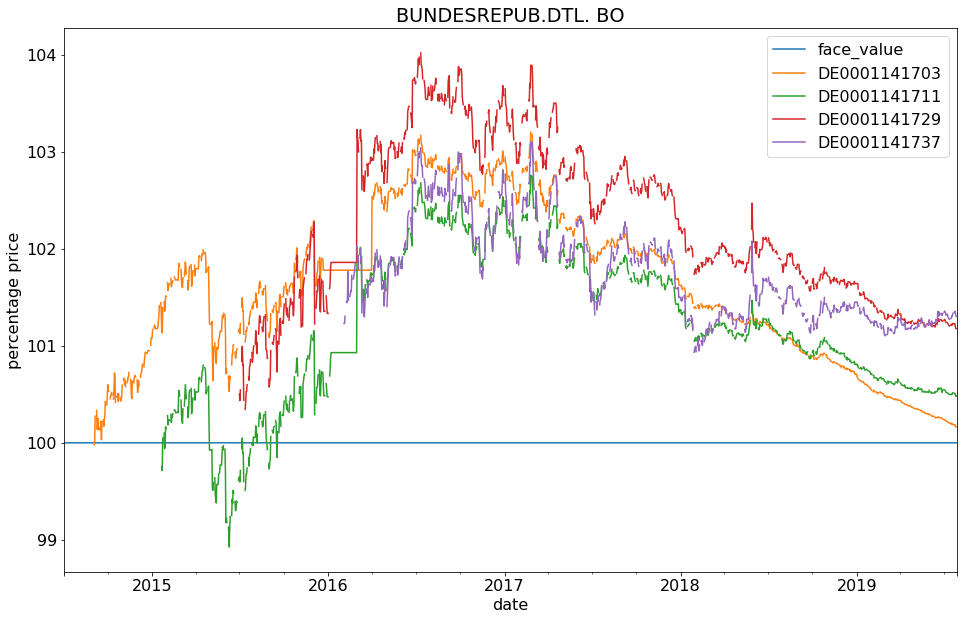
\includegraphics[width=.9\textwidth]{BUNDESREPUB_BO}
\\
\begin{tiny}
\begin{tabular}{lllllrr}

	  \textbf{bond name} &          \textbf{ISIN} & \textbf{borrower} & \textbf{issue date} & \textbf{maturity} &  \textbf{cpn} &  \textbf{red.yield}  \\

    	BUNDESREPUB.DTL.BO 2015 ZERO 17/04/20  &  DE0001141711 &         BCKKE & 2015-01-23 &           2020-04-17 &    0.00 &           -0.6459  \\
     	BUNDESREPUB.DTL.BO 2015 1/4\% 16/10/20  &  DE0001141729 &         BCKKE & 2015-07-03 &           2020-10-16 &    0.25 &           -0.6955  \\ 
      	BUNDESREPUB.DTL.BO 2014 1/4\% 11/10/19  &  DE0001141703 &         BCKKE & 2014-09-05 &           2019-10-11 &    0.25 &           -0.4781  \\ 
       	BUNDESREPUB.DTL.BO 2016 ZERO 09/01/21 &  DE0001141737 &         BCKKE & 2016-02-05 &           2021-04-09 &    0.00 &           -0.7484  \\
	
\end{tabular}
\end{tiny}
\end{tabular}
\caption{{date: 29/07/2019, source: Thomson Reuters Datastream}}
\label{fig.historicalBundPrices}
\end{figure}	
\end{center}


\begin{table}
\centering
\begin{scriptsize}
	{\rowcolors{2}{black!40!blue!10}{black!20!blue!05}
\begin{tabular}{lrrrr} 
 \textbf{bond}  &  \textbf{price  on  24/02/2017} &         \textbf{avg} &       \textbf{std} &        \textbf{vol} \\
 \hline
  DE0001141711 &              102.758 &  101.202385 &  0.774095 &         0.940906 \\
  DE0001141729 &              103.893 &  102.246960 &  0.830204 &         1.162145  \\
  DE0001141703 &              103.201 &  101.593300 &  0.806122 &          1.363008  \\
  DE0001141737 &              103.097 &  101.757502 &  0.505060 &         1.190914  
 	\end{tabular}} 
 \end{scriptsize}
\caption{{Statistics of DE00011417* }}
\label{tab.DE000stat}
\end{table}


\begin{center}
\begin{figure}
	\centering
	\begin{tabular}{c}
	\includegraphics[width=0.99\textwidth]{bridge_1d16h3m_invAndPrice} \\
		\begin{small}
			\begin{tabular}{lr | lr}
				initial inventory  $\initialInventory   $ : & 1000.0   & price process : & bridge \\
				liquidation target $\liquidationTarget   $ : & 0.0 & volatility $\sigma   $ : & 1.1642\\
				time horizon of liquidation $\timeHorizon   $ : & 1.0 & coeff marketImpact $ \coeffMarketImpact  $: & 0.05855\\
				initial price $\fundamentalPrice_0 $ : & 103.893 & 	coeff riskAversion $ \coeffRiskAversion   $ : & 0.07341 \\
			\end{tabular}
		\end{small}
	\end{tabular}
	\caption{{Simulation of bond prices and corresponding inventory trajectories}}
	\label{fig.DE000_invAndPrice}
\end{figure}
\end{center}

\newpage 



%	\subsection{Numerical experiments}\label{sec.numericalExperiment}
%	We test the strategy of Proposition \ref{prop.goodExecutionIC} and we discuss the outcomes of such numerical experiments. 
%	
%		\begin{wrapfigure}{r}{0.55\textwidth}
%		\centering
%		\includegraphics[width=0.55\textwidth]{figComparisonAposterioriAndGood}
%		\caption{\textsf{\textsf{A posteriori optimal executions and good trade executions in the regime of high volatility}}
%		\label{fig.comparisonAposterioriAndGood}
%		\end{wrapfigure}
%	
%	
%	Figure  \ref{fig.comparisonAposterioriAndGood} compares a posteriori optimal inventory trajectories with good inventory trajectories in  the case of three price realisations in the regime of high volatility. A posteriori trajectories are subject to the fuel constraint $\inventory(\timeHorizon) = \liquidationTarget$, whereas good inventory trajectories are subject to the relaxed constraint $\Expectation\inventory(\timeHorizon) = \liquidationTarget$. 
%	
%	Consider price path \#1. The price remains constantly below its expected value and the conditions are adverse to liquidation, particularly between $t\approx 0.32$ and $t\approx 0.7$. Knowing in advance the presence of the well between $t\approx 0.32$ and $t\approx 0.7$, the a posteriori solution refrains from liquidating during this period: the inventory trajectory is essentially flat and actually prescribes some acquisition in order to exploit the surge from $t\approx 0.51$ to $t\approx 0.75$. Hence, the liquidation happens at the beginning of the trading period, $0\leq t \leq 0.32$ and at the end, $0.7\leq t\leq 1$, where we observe the steepest segments of the trajectory. 
%	
%	The good trade execution, being adapted, does not benefit from the fact of knowing in advance that price path \#1 will remain below its expected value and, in particular, the presence of the well between $t\sim 0.32$ and $t\sim 0.7$. However, while the price path unfolds and such behaviour is observed, the good trade execution responds by liquidating at a slower pace than the static solution. In this way, less market impact will be exerted, in order to prevent the price from plunging even further. Moreover, the response is consistent with the direction of departure from the expected price. Indeed,  while the realised price unfolds, the trader observes it being constantly below its expected value. Having reasons to believe that the price will eventually oscillates around its expected value, the liquidation is not executed entirely but a positive amount $\inventory(\timeHorizon) - \liquidationTarget$ is left in inventory at time $\timeHorizon$, waiting for being liquidated under more favourable market conditions. 
%	
%	Consider price path \#2. The price remains above its expected value for almost all the trading period, hence constituing favourable conditions for liquidation. Knowing in advance the presence of the three spikes at $t\approx 0.21$,at $t\approx 0.49$,  and at $t\approx 0.78$, the a-posteriori solution liquidates faster around these times (steepest segments along the trajectory). It is however constrained by the rigidities at the boundary points $t=0$ and $t=\timeHorizon$ and by the risk aversion, which penalises the departure from the static optimal solution. The execution essentially finishes at around $t=0.85$, since the price after that time is no longer optimal for liquidation. 
%	
%	The good trade execution, being adapted, does not benefit from the fact of knowing in advance that price path \#2 will remain above its expected value. However, while the price path unfolds and such behaviour is observed, the good trade execution liquidates faster and sooner than the static execution. It crosses the liquidation target $\liquidationTarget=0$ between $t=0.85$ and $t=0.87$. When it does, the trader can stop the liquidation, hence emulating the a posteriori solution. 
%	
%	Consider price path \#3. The price exhibits very low volatility and it remains close to its expected trend. In such situation, both the a posteriori execution and the good trade execution are close to the static solution. 
%	
%	
%	The reciprocal positions of the good inventory trajectories \#1 and \#2 are characteristic of the type of reaction to observed prices that good trade executions permit. We emphasise that, despite being dynamic solutions, good inventory trajectories do not rely on a full SDE specification for the evolution of the asset price. This is a model robustness feature. 
%	
%	
%		\begin{wrapfigure}{r}{0.55\textwidth}
%		\centering
%		\includegraphics[width=0.55\textwidth]{figGoodInventoryProtectionAgainstAdversePriceMovements}
%		\caption{\textsf{\textsf{Good trade execution with significant terminal variance}}
%		\label{fig.GoodInventoryProtectionAgainstAdversePriceMovements}
%	\end{wrapfigure}
%	
%	
%	As observed in Remark \ref{remark.varianceOfLiquidationError}, the variance of the liquidation error depends on the variance of the fundamental price $\fundamentalPrice$ and on the parameters $\coeffMarketImpact$ and $\coeffRiskAversion$ of market impact and of risk aversion. Risk aversion in particular can be tuned to get a desired threshold of accepted liquidation error. If the difference $\inventory(\timeHorizon) - \liquidationTarget$ is allowed to be substantial, the good trade execution will considerably take into account whether the price is above or below its expected value. This is a reasonable conduct if, at the beginning of the trading period, the prediction for future price moves is trusted. 
%	
%	Consider Figure \ref{fig.GoodInventoryProtectionAgainstAdversePriceMovements}. While the price is expected to fluctuate around 100, two realisations depart from such expectation: due to high volatility, price path \#3 increases considerably, whereas price path \#4 decreases. A static solution would execute the liquidation in the same way without taking into account the actual realisations. Instead, good trade execution prescribes different responses. In the case of price path \#3, the trajectory is steeper than the static one and it hits the liquidation target at $t\approx 0.8$.  When it does, the trader can either decide to stop the liquidation (terminating the execution sooner than in the static solution) or  she can continue to follow the good inventory trajectory, gaining a short position on the asset that  she wanted to liquidate. This is explained by the considerate departure of the actual realisation of the price path from its expected value. If the prediction has to be trusted, then it is reasonable to expect that the price will decrease and the trader will benefit from her short position. 
%	
%	
%	In the case of  price path \#4 in Figure \ref{fig.GoodInventoryProtectionAgainstAdversePriceMovements} the situation is opposite. While expected to fluctuate around 100, the price plunges due to high volatility and its value at the end of he trading period is approximately 88. Such circumstances are particularly adverse to liquidation; the good trade execution hence reacts by essentially stopping the liquidation when 80\% of the inventory has been executed. In doing so, it reduces the further negative impact that it would otherwise exert on the fundamental price. This is a feature of protection against adverse price movements. In the cases of optimal static and optimal a posteriori solutions instead, the rigidity at the boundary (fuel constraint) forces the execution of the entire initial inventory and such execution plunges the impacted price to even lower levels, around 76. The impacted price in the case of good trade execution is instead approximately 83. All impacted prices are shown in Figure \ref{fig.impactedPrices} below, where the executions are compared.	
%	
%
%	
%	With respect to the same four price paths in Figure \ref{fig.GoodInventoryProtectionAgainstAdversePriceMovements}, Figure \ref{fig.revenuesFromTrade} compares the revenues from trade when trading follows optimal static execution, optimal a posteriori execution or good trade execution. Revenues from trade are computed according to formula \eqref{eq.optimisationGoodExecutionIC}.
%	
%	In the cases of price paths \#1 and \#3 (favourable conditions for liquidation), revenues from good trade executions are higher than the static counterparts. This is because of shortselling after the liquidation target is hit. In the cases of price paths \#2 and \#4 (unfavourable conditions), revenues from good trade executions are lower than the static counterparts. This is because not all the inventory has been sold: the relaxed terminal constraint $\Expectation\inventory(\timeHorizon) = \liquidationTarget$ gives flexibility to the execution, with the rationale of exerting less market impact. Having exerted less market impact, it is then reasonable to expect that the delayed execution of the remaining inventory will bring the overall revenues above those of the static solution. 
%	
% 	
%	
%	
%	\begin{figure}[h]
%		\centering
%		
%		\includegraphics[width=0.55\textwidth]{figRevenuesFromTrade}
%		\caption{\textsf{
%			\textsf{Revenues from trade corresponding to 
%				the four price paths of Figure \ref{fig.GoodInventoryProtectionAgainstAdversePriceMovements} 
%			}
%		}
%		\label{fig.revenuesFromTrade}
%	\end{figure}
%	
%	\begin{figure}[h]
%		\centering
%		\includegraphics[width=\textwidth]{figImpactedPrices}
%		\caption{\textsf{\textsf{Fundamental and Impacted prices under various executions}}
%		\label{fig.impactedPrices}
%	\end{figure}
%	


%	\vspace{3cm}




\section{Alternative risk criteria}\label{sec.alternativeRiskCriteria}
We present two alternatives to the risk aversion formulated  in equation \eqref{eq.classicalRiskAversion}. The first alternative preserves the same structure but increases the weight of the coefficient $\coeffRiskAversion$ of risk aversion linearly in time.  The second alternative is instead inspired by the value at risk for geometric Brownian motion used in \cite{GS11opt}.

\subsection{Linearly time-dependent coefficient of risk aversion}\label{sec.timeIC}
The third summand in the Lagrangian $F$ of equation \eqref{eq.lagrangianIC} accounts for the risk aversion. So far this term has been taken constant in the time variable $t$. We now propose a linear $t$-dependence, with higher risk aversion for $t$ closer to the liquidation horizon $\timeHorizon$. More precisely, we consider the Lagrangian
\begin{equation}\label{eq.lagrangianTimeIC}
F(t,S,q,r):= rS + \coeffMarketImpact\squared r\squared +\coeffRiskAversion\squared \, t \,  (q-\liquidationTarget)\squared.
\end{equation}
and we compute a good inventory trajectory for the minimisation of 
\begin{equation*}\label{eq.costFunctionalTimeIC}
\costFunctional(\eta)=\int_{0}^{\timeHorizon} F (t,\fundamentalPrice_t,\eta_t,\dotEta_t) dt, \qquad \eta \in \spaceUnbiasedInventoryTrajectoriesInitialConstraint.
\end{equation*}
The lagrangian $F$ in equation \eqref{eq.lagrangianTimeIC} satisfies the decomposition in equation \eqref{eq.abstractDecompositionOfLagrangian} and for every $t$ the function $(q,r)\mapsto F(t,S_t,q,r)$ is convex. 


Recall that $\coeffMarketImpact>0$ is the coefficient of instantaneous market impact, $\coeffRiskAversion\geq 0$ is the coefficient of risk aversion, and $\ratioAversionOverImpact=\coeffRiskAversion/\coeffMarketImpact$. The proposed time-dependency of the risk aversion is reflected in the following modifications of the norms in equations \eqref{eq.pathwiseSobolevNormIC} and \eqref{eq.sobolevNormOfInventoryTrajectoryIC}: for $\eta$ in $\sobolevSpaceOneTwo\timeWindow$ we define
\begin{equation}\label{eq.pathwiseSobolevNormTimeIC}
\lvert \eta \rvert \squared _{\coeffMarketImpact,\coeffRiskAversion\sqrt{t}}:= \intZeroTimeHorizon (\coeffRiskAversion\squared t \eta\squared_t + \coeffMarketImpact\squared \dotEta\squared_t) dt;
\end{equation}
for $\inventory$ in $\spaceUnbiasedInventoryTrajectoriesInitialConstraint$ we define
\begin{equation}\label{eq.sobolevNormTimeIC}
\lVert \inventory \rVert\squared_{\coeffMarketImpact,\coeffRiskAversion\sqrt{t} }
:=
\Expectation \left[ \lvert \inventory \rvert_{\coeffMarketImpact,\coeffRiskAversion\sqrt{t}}\squared \right].
\end{equation}
Consequently, this section's counterpart to the static tubular neighbourhood in equation \eqref{eq.staticTubularNeighbourhoodIC} is  
\begin{equation}\label{eq.staticTubularNeighbourhoodTimeIC}
\spaceUnbiasedInventoryTrajectoriesInitialConstraint (\inventory, C):=
\left\lbrace
\eta \in \spaceUnbiasedInventoryTrajectoriesInitialConstraint: \, 
\norm[\eta_\timeHorizon -\inventory_\timeHorizon]_{\Ltwo(\Prob)} \leq 
C \lVert \eta -\inventory\rVert\squared_{\coeffMarketImpact,\coeffRiskAversion\sqrt{t} }
\right\rbrace,
\end{equation}
and  this section's counterpart to the pathwise tubular neighbourhood in equation \eqref{eq.pathwiseTuburalNeighbourhoodIC} is 
\begin{equation}
\begin{split}\label{eq.pathwiseTubularNeighbourhoodTimeIC}
\spaceUnbiasedInventoryTrajectoriesInitialConstraint_{\text{pw}}(\inventory,\xi):=
\Big\lbrace
\eta \in \spaceInventoryTrajectories: \, 
\abs{\eta_\timeHorizon-\inventory_\timeHorizon} 
&\leq \xi\lvert \eta - \inventory\rvert \squared_{\coeffMarketImpact,\coeffRiskAversion\sqrt{t} }
\Big\rbrace.
\end{split}
\end{equation}

The definition of the good trade execution $\inventory$ in $\spaceUnbiasedInventoryTrajectoriesInitialConstraint$ for the minimisation of the cost functional $\costFunctional$ in equation \eqref{eq.costFunctionalTimeIC} with the lagrangian $F$ as in equation \eqref{eq.lagrangianTimeIC} is as in Definition \ref{defi.goodTradeExecution}, where however the neighbourhoods $\spaceUnbiasedInventoryTrajectoriesInitialConstraint (\inventory_\timeHorizon, C)$ and $\spaceUnbiasedInventoryTrajectoriesInitialConstraint_{\text{pw}}(\inventory_\timeHorizon,\xi)$ are those in equations \eqref{eq.staticTubularNeighbourhoodTimeIC} and \eqref{eq.pathwiseTubularNeighbourhoodTimeIC} respectively, rather than those in equations \eqref{eq.staticTubularNeighbourhoodIC} and \eqref{eq.pathwiseTuburalNeighbourhoodIC}.

Having formulated the concept of good trade execution in the present case of time-dependent coefficient of risk-aversion, we now proceed as done in Sections \ref{sec.statementOfGoodTradeExecutionIC} and \ref{sec.eulerLagrangeIC}, namely: in Proposition \ref{prop.goodTradeExecutionTimeIC} we give a close form formula for a good trade execution for the minimisation of the cost functional $\costFunctional$ in \eqref{eq.costFunctionalTimeIC}; then in Lemma \ref{lemma.uniquenessOfSolutionEulerLagrangeTimeIC} and in Proposition \ref{prop.characterisationEulerLagrangeTimeIC} we show that in fact such a good trade execution is unique and we characterise it as the solution of a random Young differential equation. In order to shorten the notation we take $\liquidationTarget = 0$ and we omit this from the formulas. 

\begin{prop}[``Closed-form formula for the good trade execution under linearly time dependent risk criterion'']\label{prop.goodTradeExecutionTimeIC}
Let $\airyFirstFunction$ and $\airySecondFunction$ be the first and the second Airy's functions, namely the two independent solutions to the second order linear ordinary differential equation $u^{\prime \prime}(t) - tu(t) = 0$. Moreover, set
\begin{equation*}
\begin{split}
\alpha(t) =& \airyFirstFunction(\ratioAversionOverImpact^{2/3} t),\\
\beta(t) =& \airySecondFunction(\ratioAversionOverImpact^{2/3} t), \\
\phi(t) =& \frac{1}{2\coeffMarketImpact\squared}\intzerot \alpha^{-2}(s)\int_{0}^{s}\alpha(u)d\fundamentalPrice_u \,ds,
\end{split}
\end{equation*}
where the innermost integral in the definition of $\phi$ is the Young integral introduced in Appendix \ref{sec.eulerLagrangeInPresenceOfPricePath}.
Define the constants $c_A$ and $c_B$ as follows
\begin{equation*}
c_A = \frac{\beta(\timeHorizon)\initialInventory - \alpha(\timeHorizon)\beta(0)\Expectation\phi(\timeHorizon)}
{\alpha(0)\beta(\timeHorizon) - \alpha(\timeHorizon)\beta(0)},
\end{equation*}
	\begin{equation*}
c_B = \frac{ \alpha(\timeHorizon)}
{\alpha(0)\beta(\timeHorizon) - \alpha(\timeHorizon)\beta(0)}\Big(\alpha(0)\Expectation\phi(\timeHorizon) - \initialInventory\Big).
\end{equation*}
Then, the inventory trajectory 
\begin{equation}\label{eq.goodTradeExecutionTimeIC}
\inventory_t = c_A \alpha(t) + c_B\beta(t) - \alpha(t) \phi(t)
\end{equation}
is a $(C,\xi)$-good trade execution, where
\begin{equation*}
C=1/
\lVert 
\fundamentalPrice_{\timeHorizon} - 2\coeffMarketImpact\squared \dot{\alpha \phi}(\timeHorizon) 
\rVert_{\Ltwo(\Prob)},
\end{equation*}
\begin{equation*}
\xi=1/
\lvert 
\fundamentalPrice_{\timeHorizon} 
+2\coeffMarketImpact\squared c_A\dot{\alpha}(\timeHorizon)
+2\coeffMarketImpact\squared c_B \dot{\beta}(\timeHorizon)
-2\coeffMarketImpact\squared \dot{\alpha \phi}(\timeHorizon)
\rvert,
\end{equation*}
where the symbol $ \dot{\alpha \phi}$ denotes the time derivative of the product function $t\mapsto\alpha(t)\phi(t)$. 
\end{prop}
\begin{proof}
The proof is conducted along the same lines of the proof of Proposition \ref{prop.goodExecutionIC}.
Let $\inventory$ be as in equation \eqref{eq.goodTradeExecutionTimeIC}. It is straightforward to check that indeed $\inventory$ is in $\spaceUnbiasedInventoryTrajectoriesInitialConstraint$. 
 Let $f_t:= 2\coeffMarketImpact\squared \inventoryRate_{t} + \fundamentalPrice_t$ and notice that $f$ is absolutely continuous with derivative 
\begin{equation}\label{eq.eulerLagrangeWithCancellationTimeIC}
\dot{f}_t = 2 \coeffMarketImpact\squared t \inventory_t .
\end{equation}
Let $\eta$ be in $\spaceUnbiasedInventoryTrajectoriesInitialConstraint$. We write $e$ for the difference $e:=\eta-\inventory$, and we observe that $e_0=0$ and $\Expectation e_\timeHorizon = 0$.  Then, we have 
\begin{equation*}
\begin{split}
\costFunctional(\eta) - \costFunctional(\inventory) = &
\intZeroTimeHorizon \Big[ f_t \dot{e}_t + 2\coeffMarketImpact\squared t \inventory_t \, e_t\Big]dt\\
&+\int_{0}^{\timeHorizon}\big(\coeffMarketImpact\squared \dot{e}_t\squared + \coeffRiskAversion\squared \, t \, e\squared_t \big)dt.
\end{split}
\end{equation*}
The second integral on the right hand side is $ \lvert e \rvert_{\coeffMarketImpact,\coeffRiskAversion\sqrt{t}}\squared$.  
Using integration by parts we see that in fact $\costFunctional(\eta) - \costFunctional(\inventory) $ $= f_\timeHorizon e_\timeHorizon $ $ + \lvert e \rvert_{\coeffMarketImpact,\coeffRiskAversion\sqrt{t}}\squared$, because of equation \eqref{eq.eulerLagrangeWithCancellationTimeIC}.  
Therefore, the difference $\costFunctional(\eta) - \costFunctional(\inventory) $ is non-negative if 
\begin{equation*}
\abs{e_\timeHorizon}
\leq \frac{ \lvert e \rvert_{\coeffMarketImpact,\coeffRiskAversion}\squared}{\abs{f_\timeHorizon}}.
\end{equation*}
This gives $\xi = 1/\lvert f_\timeHorizon\rvert$.

Secondly, consider the   expected difference $\Expectation \costFunctional (\eta) - \Expectation \costFunctional (\inventory)$ $=\Expectation[f_\timeHorizon e_\timeHorizon] + \normInventoryTrjectories{e}\squared$. We can estimate
\begin{equation*}
\Expectation[f_\timeHorizon e_\timeHorizon] \leq \Variance^{\half}(f_\timeHorizon)\norm[e_\timeHorizon]_{\Ltwo(\Prob)},
\end{equation*}
because $\Expectation e_\timeHorizon = 0$. We have  
\begin{equation*}
\Variance(f_\timeHorizon)
= \lVert \fundamentalPrice_\timeHorizon - 2\coeffMarketImpact\squared \dot{\alpha\phi} (\timeHorizon) \rVert_{\Ltwo(\Prob)}^{2}. 
\end{equation*} 
Therefore, the   expected difference $\Expectation \costFunctional (\eta) - \Expectation \costFunctional (\inventory)$ is non-negative if 
\begin{equation*}
\norm[e_\timeHorizon]_{\Ltwo(\Prob)} \leq 
\frac{ \lVert e \rVert_{\coeffMarketImpact, \coeffRiskAversion\sqrt{t}} \squared }{\lVert \fundamentalPrice_\timeHorizon - 2\coeffMarketImpact\squared \dot{\alpha\phi} (\timeHorizon) \rVert_{\Ltwo(\Prob)}}.
\end{equation*}
This gives the constant $C$ in the statement and concludes the proof.
%		
%		
%		
%		
%		
%		 and let $\momentumOfExecution$ be its momentum of execution, defined by
%		$
%		\momentumOfExecution:=\coeffMarketImpact\squared \inventoryRate.
%		$
%		Notice that 
%		\begin{equation}\label{eq.EulerLagrangeWithTimeDependentRiskAversion}
%		d\momentumOfExecution = \coeffRiskAversion\squared  t \,  \inventory dt 
%		-d\fundamentalPrice/2 .
%		\end{equation}
%		Let $\eta$ be in $\spaceInventoryTrajectories$. We write $e$ for the difference $e:=\eta-\inventory$ and we observe $\Expectation e (\timeHorizon) = 0$. Moreover, we write $\costFunctional(\eta):=\int_{0}^{\timeHorizon} \lagrangian(t,\eta(t),\dot{\eta}(t) )dt$, where the Lagrangian $\lagrangian$ is defined in equation \eqref{eq.lagrangianWithTimeDependentRiskAversion}. Then, by using integration by parts, we have 
%		\begin{equation*}
%		\begin{split}
%		\costFunctional(\eta) - \costFunctional(\inventory) = &
%		\Big[\fundamentalPrice_{\timeHorizon} + 2 \momentumOfExecution(\timeHorizon)\Big] e(\timeHorizon) \\
%		&+\int_{0}^{\timeHorizon} e \big\lbrace 2\coeffRiskAversion\squared t \inventory  dt 
%		-d\fundamentalPrice - 2 d\momentumOfExecution \big\rbrace \\
%		&+\int_{0}^{\timeHorizon}\big(\coeffMarketImpact\squared \dot{e}\squared + \coeffRiskAversion\squared t \,  e\squared \big)dt.
%		\end{split}
%		\end{equation*}
%		The second summand vanishes because of \eqref{eq.EulerLagrangeWithTimeDependentRiskAversion}. Therefore, the difference $\costFunctional(\eta) - \costFunctional(\inventory)$ is non-negative if $\eta$ is in $\spaceInventoryTrajectories_{\text{pw}}(\inventory(\timeHorizon),\xi)$ with $\xi= 1/ $ $ \lvert\fundamentalPrice_{\timeHorizon} + 2 \momentumOfExecution(\timeHorizon)\rvert$. 
%		
%		
%		 Moreover, the expected difference $\Expectation \costFunctional (\eta) - \Expectation \costFunctional (\inventory)$ is non-negative if 
%		\[
%		\Expectation\left[
%		e(\timeHorizon) \Big(\fundamentalPrice_{\timeHorizon} + 2 \momentumOfExecution(\timeHorizon)\Big)
%		\right]
%		+\lVert{e}\rVert\squared_{\coeffMarketImpact,\coeffRiskAversion\sqrt{t}} \geq 0,
%		\]
%		which holds in particular if 
%		\[
%		\norm[e(\timeHorizon)]_{\Ltwo(\Prob)} \leq 
%		\frac{\lVert{e}\rVert\squared_{\coeffMarketImpact,\coeffRiskAversion\sqrt{t}}}
%		{	\lVert
%			\fundamentalPrice_{\timeHorizon} - 2\coeffMarketImpact\squared \dot{\alpha}(\timeHorizon)\phi(\timeHorizon) - 2\coeffMarketImpact\squared \alpha(\timeHorizon)\dot{\phi}(\timeHorizon)
%			\rVert_{\Ltwo(\Prob)}
%		}.
%		\]
%		This gives 
%		$
%		C=1/
%		\lVert 
%		\fundamentalPrice_{\timeHorizon} - 2\coeffMarketImpact\squared \dot{\alpha \phi}(\timeHorizon) 
%		\rVert_{\Ltwo(\Prob)}.
%		$
\end{proof}

The Lagrangian $F$ in equation \eqref{eq.lagrangianTimeIC} satisfies the assumptions in Proposition \ref{prop.eulerLagrangeNecessity}; equation \eqref{eq.strongFormEulerLagrangeEquation} in the present case reads
\begin{equation}\label{eq.eulerLagrangeSystemTimeIC}
\begin{cases}
d\inventory_t=r_{t} dt \\
dr_{t} = \ratioAversionOverImpact\squared \, t \, \inventory_t dt - d\fundamentalPrice_t / 2\coeffMarketImpact\squared
\end{cases}
\end{equation}
We now characterise the good trade execution in Proposition \ref{prop.goodTradeExecutionTimeIC} as the unique solution to the random Young differential equation \eqref{eq.eulerLagrangeSystemTimeIC}.

\begin{lemma}\label{lemma.uniquenessOfSolutionEulerLagrangeTimeIC}
Let $\inventory$ and $\tilde{\inventory}$ be two solutions to equation \eqref{eq.eulerLagrangeSystemTimeIC}. Then, the difference $\inventory - \tilde{\inventory}$ is deterministic. As a consequence, the solution to the equation \eqref{eq.eulerLagrangeSystemTimeIC} with constraint
\begin{equation}\label{eq.initialAndTerminalCOnditionsTimeIC}
\begin{cases}
\inventory_0 = \initialInventory \\
\Expectation \inventory_\timeHorizon = \liquidationTarget = 0 
\end{cases}
\end{equation}
is unique.
\end{lemma}
\begin{proof}
The proof is conducted along the same lines as the proofs of Lemma \ref{lemma.twoSolutionsEulerLagrangeIC} and Lemma \ref{lemma.uniquenessOfEulerLagrangeIC}. 
\end{proof}

\begin{prop} [``Characterisation of good trade execution via Euler-Lagrange equation''] \label{prop.characterisationEulerLagrangeTimeIC}
The good trade execution of Proposition \ref{prop.goodTradeExecutionTimeIC} is characterised as the unique solution to the random Young differential equation \eqref{eq.eulerLagrangeSystemTimeIC} with initialisation
\begin{equation*}
\begin{cases}
\inventory_0 = \initialInventory \\
r_0 = e_A(0) \alpha_0 + e_B (0) \beta_0,
\end{cases}
\end{equation*}
where $\alpha$ and $\beta$ are as in Proposition \ref{prop.goodTradeExecutionTimeIC}, and 
\begin{equation*}
\begin{split}
e_A (0) =& \frac{ \beta_\timeHorizon \initialInventory - \beta_0 \tilde{K}}{\alpha_0\beta_\timeHorizon - \alpha_\timeHorizon \beta_0} \\
e_B (0) =& \frac{\alpha_0 \tilde{K} - \alpha_\timeHorizon \initialInventory}{\alpha_0\beta_\timeHorizon - \alpha_\timeHorizon \beta_0} \\
\tilde{K} = & \frac{\fundamentalPrice_0}{2\coeffMarketImpact\squared W_0}\left(\alpha_\timeHorizon \beta_0 - \alpha_0 \beta_\timeHorizon \right) \\
%		& \frac{\alpha_\timeHorizon}{2\coeffMarketImpact\squared} \intZeroTimeHorizon \Expectation\left[\fundamentalPrice_u\right] \frac{d}{d u} \left(\frac{\beta_u}{W_u}\right) du \\
%		& - \frac{\beta_\timeHorizon}{2\coeffMarketImpact\squared} \intZeroTimeHorizon \Expectation\left[\fundamentalPrice_u\right] \frac{d}{d u} \left(\frac{\alpha_u}{W_u}\right) du\\
& + \frac{1}{2\coeffMarketImpact\squared} \intZeroTimeHorizon \Expectation\left[\fundamentalPrice_u\right] 
\frac{d}{d u} \left(\frac{\alpha_\timeHorizon \beta_u - \beta_\timeHorizon \alpha_u}{W_u}\right) du \\
W_t = & \alpha_t \dot{\beta}_t - \dot{\alpha}_t \beta_t. 
\end{split}
\end{equation*}
In particular, the good trade execution in Proposition \ref{prop.goodTradeExecutionTimeIC} is the only good trade execution for the minimisation of \eqref{eq.costFunctionalTimeIC} with the Lagrangian $F$ as in equation \eqref{eq.lagrangianTimeIC}.
\end{prop}
\begin{proof}
The proof is conducted along the same lines of the proof of Proposition \ref{prop.eulerLagrangeCharacterisationIC}, relying  on Lemma \ref{lemma.uniquenessOfSolutionEulerLagrangeTimeIC} above and on Proposition \ref{prop.eulerLagrangeNecessity} in the Appendix. In particular, if we set $Y=(q,r)\transpose$ and $\mu=\Expectation[Y]$, then $\mu$ solves the ordinary differential equation 
\begin{equation}\label{eq.ODEexpectedTrajectoryTimeIC}
\begin{cases}
\dot{\mu}^{(1)}_t = \mu^{(2)}_t \\
\dot{\mu}^{(2)}_t = \ratioAversionOverImpact\squared \, t \, \mu^{(1)}_t - \varphi_t/2\coeffMarketImpact\squared,
\end{cases}
\end{equation}
where $\varphi_t=d\Expectation[\fundamentalPrice_t]/dt$. The map $t\mapsto \Expectation[\fundamentalPrice_t]$ is temporarily assumed to be differentiable; at the end of the argument a standard approximation argument can be used to extend the findings to the general case. The general solution to equation \eqref{eq.ODEexpectedTrajectoryTimeIC} is 
\begin{equation*}
\begin{cases}
\mu^{(1)}_t = e_A (t)\alpha_t + e_B(t)\beta_t \\
\mu^{(2)}_t = e_A(t)\dot{\alpha}_t + e_B(t)\dot{\beta}_t,
\end{cases}
\end{equation*}
where $\alpha$ and $\beta$ are as in Proposition \ref{prop.goodTradeExecutionTimeIC} and
\begin{equation*}
\begin{split}
e_A(t) = & 
e_A(0) + \frac{1}{2\coeffMarketImpact\squared} \left(\frac{\beta_t}{W_t} \Expectation[\fundamentalPrice_t] - \frac{\beta_0}{W_0}\fundamentalPrice_0\right) \\
& -\frac{1}{2\coeffMarketImpact\squared}\intzerot \Expectation[\fundamentalPrice_u]\frac{d}{du}\left(\frac{\beta_u}{W_u}\right)du\\
e_B(t) = & 
e_B(0) - \frac{1}{2\coeffMarketImpact\squared} \left(\frac{\alpha_t}{W_t} \Expectation[\fundamentalPrice_t] - \frac{\alpha_0}{W_0}\fundamentalPrice_0\right) \\
& +\frac{1}{2\coeffMarketImpact\squared}\intzerot \Expectation[\fundamentalPrice_u]\frac{d}{du}\left(\frac{\alpha_u}{W_u}\right)du,
\end{split}
\end{equation*}
where $W$ is the Wronskian $W_t = \alpha_t\dot{\beta}_t - \dot{\alpha}_t \beta_t$. Choosing the constants $e_A(0)$ and $e_B(0)$ as in the statement guarantees that the constraints in equation \eqref{eq.initialAndTerminalCOnditionsTimeIC} are satisfied. 
\end{proof}

\subsection{VaR-inspired risk criterion}\label{sec.varInspiredRiskCriterion}
In \cite{GS11opt}, the authors model the fundamental price $\fundamentalPrice$ as a geometric Brownian motion and they adopt the value at risk as measure of risk aversion. This means penalising the revenues from trade of equation \eqref{eq.revenuesFromTrade} by subtracting a term proportional to $\inventory_t \fundamentalPrice_t$ at every time $t$. Inspired by their modelling choices, we now discuss the minimisation of 
\begin{equation}\label{eq.costFunctionalVaR}
\costFunctional(\inventory)=
\int_{0}^{\timeHorizon} 
\Big(
 \inventoryRate_{t} \fundamentalPrice_t + \coeffMarketImpact\squared \inventoryRate_{t}\squared + \coeffRiskAversion\squared \inventory_t \fundamentalPrice_t
\Big)
dt,
\end{equation}
over $\inventory$ in $\spaceUnbiasedInventoryTrajectoriesInitialConstraint$. However, we do not assume any SDE dynamics for the price process, which retains the generality of the previous sections. Compared to the former lagrangians in equations \eqref{eq.lagrangianIC} and \eqref{eq.lagrangianTimeIC}, the lagrangian $F(t,S,q,r)= r S + \coeffMarketImpact\squared r\squared + \coeffRiskAversion\squared q \fundamentalPrice$ in the functional $\costFunctional$ of equation \eqref{eq.costFunctionalVaR}  no longer has the quadratic term in $q$. This is reflected
 in the following modifications of the norms in equations \eqref{eq.pathwiseSobolevNormIC} and \eqref{eq.sobolevNormOfInventoryTrajectoryIC}: for $\eta$ in $\sobolevSpaceOneTwo\timeWindow$ we define
\begin{equation}\label{eq.pathwiseSobolevNormVaR}
\lvert \eta \rvert \squared _{\coeffMarketImpact}:= \intZeroTimeHorizon \coeffMarketImpact\squared \dotEta\squared_t dt;
\end{equation}
for $\inventory$ in $\spaceUnbiasedInventoryTrajectoriesInitialConstraint$ we define
\begin{equation}\label{eq.sobolevNormVaR}
\lVert \inventory \rVert\squared_{\coeffMarketImpact}
:=
\Expectation \left[ \lvert \inventory \rvert_{\coeffMarketImpact}\squared \right].
\end{equation}
Consequently, this section's counterpart to the static tubular neighbourhood in equation \eqref{eq.staticTubularNeighbourhoodIC} is  
\begin{equation}\label{eq.staticTubularNeighbourhoodVaR}
\spaceUnbiasedInventoryTrajectoriesInitialConstraint (\inventory, C):=
\left\lbrace
\eta \in \spaceUnbiasedInventoryTrajectoriesInitialConstraint: \, 
\norm[\eta_\timeHorizon -\inventory_\timeHorizon]_{\Ltwo(\Prob)} \leq 
C \lVert \eta -\inventory\rVert\squared_{\coeffMarketImpact }
\right\rbrace,
\end{equation}
and  this section's counterpart to the pathwise tubular neighbourhood in equation \eqref{eq.pathwiseTuburalNeighbourhoodIC} is 
\begin{equation}
\begin{split}\label{eq.pathwiseTubularNeighbourhoodVaR}
\spaceUnbiasedInventoryTrajectoriesInitialConstraint_{\text{pw}}(\inventory,\xi):=
\Big\lbrace
\eta \in \spaceInventoryTrajectories: \, 
\abs{\eta_\timeHorizon-\inventory_\timeHorizon} 
&\leq \xi\lvert \eta - \inventory\rvert \squared_{\coeffMarketImpact}
\Big\rbrace.
\end{split}
\end{equation}

The definition of the good trade execution $\inventory$ in $\spaceUnbiasedInventoryTrajectoriesInitialConstraint$ for the minimisation of the cost functional $\costFunctional$ in equation \eqref{eq.costFunctionalVaR}  is as in Definition \ref{defi.goodTradeExecution}, where however the neighbourhoods $\spaceUnbiasedInventoryTrajectoriesInitialConstraint (\inventory_\timeHorizon, C)$ and $\spaceUnbiasedInventoryTrajectoriesInitialConstraint_{\text{pw}}(\inventory_\timeHorizon,\xi)$ are those in equations \eqref{eq.staticTubularNeighbourhoodVaR} and \eqref{eq.pathwiseTubularNeighbourhoodVaR} respectively, rather than those in equations \eqref{eq.staticTubularNeighbourhoodIC} and \eqref{eq.pathwiseTuburalNeighbourhoodIC}.

Having formulated the concept of good trade execution in the present case of VaR-inspired risk-aversion, we now proceed as done in Sections \ref{sec.statementOfGoodTradeExecutionIC} and \ref{sec.eulerLagrangeIC}, namely: in Proposition \ref{prop.goodTradeExecutionVaR} we give a close form formula for a good trade execution for the minimisation of the cost functional $\costFunctional$ in \eqref{eq.costFunctionalVaR}; then in Lemma \ref{lemma.uniquenessOfSolutionEulerLagrangeVaR} and in Proposition \ref{prop.characterisationEulerLagrangeVaR} we show that in fact such a good trade execution is unique and we characterise it as the solution of a random Young differential equation.	

\begin{prop}[``Closed-form formula for the good trade execution under VaR-inspired risk criterion'']\label{prop.goodTradeExecutionVaR}
	Let $K$ be the constant 
	\begin{equation*}
	K=\frac{1}{2\coeffMarketImpact\squared \timeHorizon}\int_{0}^{\timeHorizon} 
	\left(
	\Expectation\left[\fundamentalPrice_s\right] - \coeffRiskAversion\squared \int_{0}^{s}\Expectation\left[\fundamentalPrice_u\right]du 
	 \right) ds.
	\end{equation*}
	Then, the inventory trajectory 
	\begin{equation}\label{eq.goodExecutionVaR}
	\begin{split}
	\inventory_t =& \left(1-\frac{t}{\timeHorizon}\right)\initialInventory + \frac{t}{\timeHorizon}\liquidationTarget \\
	& - \frac{1}{2\coeffMarketImpact\squared}\int_{0}^{t} 
	\left(
	\fundamentalPrice_s - \coeffRiskAversion\squared \int_{0}^{s}\fundamentalPrice_u du 
	\right) ds\\
	& +Kt
	\end{split}
	\end{equation}
	is a $(C,\xi)$-good trade execution for the minimisation of $J$ in equation \eqref{eq.costFunctionalVaR}. The random variable $\xi$ is explicitly given by the formula  
	\begin{equation*}
	\xi\inverse  = \left\lvert
	\frac{2\coeffMarketImpact\squared}{\timeHorizon} \big(\liquidationTarget - \initialInventory \big)
	+2\coeffMarketImpact\squared K 
	+\coeffRiskAversion\squared \int_{0}^{\timeHorizon} \fundamentalPrice_t dt 
	\right\rvert
	\end{equation*}
	and the constant $C$ is explicitly given by the formula $C\inverse=\lVert \xi\inverse \rVert_{\Ltwo(\Prob)}$. 
\end{prop}
\begin{proof}
The proof is conducted along the same lines of the proof of Proposition \ref{prop.goodExecutionIC}.
Let $\inventory$ be as in equation \eqref{eq.goodExecutionVaR}. It is straightforward to check that indeed $\inventory$ is in $\spaceUnbiasedInventoryTrajectoriesInitialConstraint$. 
As done in the proof of Proposition \ref{prop.goodExecutionIC} and in the proof of Proposition \ref{prop.goodTradeExecutionTimeIC}, we let 
 $f_t:= 2\coeffMarketImpact\squared \inventoryRate_{t} + \fundamentalPrice_t$ and we observe that   that $f$ is absolutely continuous. In the present case the derivative of $f$ is  
\begin{equation}\label{eq.eulerLagrangeWithCancellationVaR}
\dot{f}_t =\coeffMarketImpact\squared \fundamentalPrice_t .
\end{equation}
Let $\eta$ be in $\spaceUnbiasedInventoryTrajectoriesInitialConstraint$. We write $e$ for the difference $e:=\eta-\inventory$, and we observe that
\begin{equation*}
\begin{split}
\costFunctional(\eta) - \costFunctional(\inventory) = &
\intZeroTimeHorizon \Big[ f_t \dot{e}_t + \coeffMarketImpact\squared\fundamentalPrice_t \, e_t\Big]dt\\
&+\int_{0}^{\timeHorizon}\coeffMarketImpact\squared \dot{e}_t\squared dt.
\end{split}
\end{equation*}
The second integral on the right hand side is $ \lvert e \rvert_{\coeffMarketImpact}\squared$.  
Using integration by parts we see that in fact $\costFunctional(\eta) - \costFunctional(\inventory) $ $= f_\timeHorizon e_\timeHorizon $ $ + \lvert e \rvert_{\coeffMarketImpact}\squared$, because of equation \eqref{eq.eulerLagrangeWithCancellationVaR}.  Therefore the conclusion is reached as done in the proof of Proposition  \ref{prop.goodExecutionIC} and in the proof of Proposition \ref{prop.goodTradeExecutionTimeIC}.
\end{proof}

\begin{remark}
The good trade execution in equation \eqref{eq.goodExecutionVaR} has the same structure of the one in equation \eqref{eq.goodExecutionIC}, namely: a time-dependent convex combination of $\initialInventory$ and $\liquidationTarget$ (first line), a dynamic response to the realisation of the price path (second line), and an adjustment for the constraint $\Expectation\inventory_\timeHorizon = \liquidationTarget$ (third line). Moreover, notice that 
\begin{equation*}
\lim_{\coeffRiskAversion\downarrow 0}
\frac{\sinh\left(\frac{\coeffRiskAversion}{\coeffMarketImpact} (\timeHorizon - t)\right)}{\sinh\left(\frac{\coeffRiskAversion}{\coeffMarketImpact} \timeHorizon \right)}
= 1 - 	\lim_{\coeffRiskAversion\downarrow 0}
\frac{\sinh\left(\frac{\coeffRiskAversion}{\coeffMarketImpact}  t\right)}{\sinh\left(\frac{\coeffRiskAversion}{\coeffMarketImpact} \timeHorizon \right)}
= 1- \frac{t}{\timeHorizon},
\end{equation*} 
so that the good trade execution in equation \eqref{eq.goodExecutionVaR} and the good trade execution in equation \eqref{eq.goodExecutionIC} agree when the risk aversion vanishes, i.e. in the limit as $\coeffRiskAversion\downarrow 0$. 
\end{remark}

\begin{remark}
Of the good trade execution in equation \eqref{eq.goodExecutionVaR}, we can compute 
\begin{equation*}
\lVert \inventory_\timeHorizon - \liquidationTarget \rVert_{\Ltwo(\Prob)}
= \frac{1}{2\coeffMarketImpact\squared} 
\Expectation^{\half} \Big[
\big(
\int_{0}^{\timeHorizon}
	\Big\lbrace
		\coeffRiskAversion\squared \intzerot (\fundamentalPrice_u - \Expectation[\fundamentalPrice_u])du 
		-  (\fundamentalPrice_t - \Expectation[\fundamentalPrice_t])
	\Big\rbrace dt 
\big)\squared 
\Big]
\end{equation*}
and estimate 
\begin{equation*}
\Variance(\inventory_\timeHorizon) \leq 
\frac{\timeHorizon}{2\coeffMarketImpact^{4}} \int_{0}^{\timeHorizon}
\left(
\coeffRiskAversion^{4} t \intzerot \Variance(\fundamentalPrice_u)du + \Variance(\fundamentalPrice_t)
\right)dt.
\end{equation*}
Therefore, the two facts presented in Remark \ref{remark.varianceOfLiquidationError} also holds for the good trade execution of Proposition \ref{prop.goodTradeExecutionVaR}.
\end{remark}

Let $F(t,S,q,r)= r S + \coeffMarketImpact\squared r\squared + \coeffRiskAversion\squared q \fundamentalPrice$ be the lagrangian in the cost functional of equation \eqref{eq.costFunctionalVaR}. Then,$F$  satisfies the assumptions in Proposition \ref{prop.eulerLagrangeNecessity}; equation \eqref{eq.strongFormEulerLagrangeEquation} in the present case reads
\begin{equation}\label{eq.eulerLagrangeSystemVaR}
\begin{cases}
d\inventory_t=r_{t} dt \\
dr_{t} = \ratioAversionOverImpact\squared \, t \, \fundamentalPrice_t dt/2 - d\fundamentalPrice_t / 2\coeffMarketImpact\squared
\end{cases}
\end{equation}

We now characterise the good trade execution in Proposition \ref{prop.goodTradeExecutionVaR} as the unique solution to the random Young differential equation \eqref{eq.eulerLagrangeSystemVaR}. Observe that equation \eqref{eq.eulerLagrangeSystemVaR} is solved by direct integration and this simplifies several calculations compared to the cases of Sections \ref{sec.eulerLagrangeIC} and \ref{sec.timeIC}. 

\begin{lemma}\label{lemma.uniquenessOfSolutionEulerLagrangeVaR}
Let $\inventory$ and $\tilde{\inventory}$ be two solutions to equation \eqref{eq.eulerLagrangeSystemVaR}. Then, the difference $\inventory - \tilde{\inventory}$ is deterministic. As a consequence, the solution to the equation \eqref{eq.eulerLagrangeSystemVaR} with constraint
\begin{equation}\label{eq.initialAndTerminalCOnditionsVaR}
\begin{cases}
\inventory_0 = \initialInventory \\
\Expectation \inventory_\timeHorizon = \liquidationTarget = 0 
\end{cases}
\end{equation}
is unique.
\end{lemma}
\begin{proof}
The proof is conducted along the same lines as the proofs of Lemma \ref{lemma.twoSolutionsEulerLagrangeIC} and Lemma \ref{lemma.uniquenessOfEulerLagrangeIC}. 
\end{proof}

\begin{prop}[``Characterisation of good trade execution via Euler-Lagrange equation'']\label{prop.characterisationEulerLagrangeVaR}
The good trade execution of Proposition \ref{prop.goodTradeExecutionVaR} is characterised as the unique solution to the random Young differential equation \eqref{eq.eulerLagrangeSystemVaR} with initialisation
\begin{equation*}
\begin{cases}
\inventory_0 =& \initialInventory \\
r_0 =& \frac{\liquidationTarget - \initialInventory}{\timeHorizon}  +\frac{1}{2\coeffMarketImpact\squared \timeHorizon} \intZeroTimeHorizon \left(\Expectation[\fundamentalPrice_t] - \fundamentalPrice_0 - \coeffRiskAversion\squared \intzerot \Expectation[\fundamentalPrice_u]du\right)dt.
\end{cases}
\end{equation*}
In particular, the good trade execution in Proposition \ref{prop.goodTradeExecutionVaR} is the only good trade execution for the minimisation of \eqref{eq.costFunctionalVaR}.
\end{prop}
\begin{proof}
The proof is conducted along the same lines of the proof of Proposition \ref{prop.eulerLagrangeCharacterisationIC}, relying  on Lemma \ref{lemma.uniquenessOfSolutionEulerLagrangeVaR} above and on Proposition \ref{prop.eulerLagrangeNecessity} in the Appendix. For the determination of the initial conditions to the Young differential equation \eqref{eq.eulerLagrangeSystemVaR}, it suffices to notice that, if we set $Y=(q,r)\transpose$ and $\mu=\Expectation[Y]$, then we have
\begin{equation*}
\begin{cases}
\mu^{(1)}_t = \initialInventory + \intzerot \mu^{(2)}_s ds \\
\mu^{(2)}_t = r_0 - \frac{1}{2\coeffMarketImpact\squared} \left(\Expectation[\fundamentalPrice_t] -\fundamentalPrice_0 - \coeffRiskAversion\squared \intzerot \Expectation[\fundamentalPrice_u]du \right).
\end{cases}
\end{equation*}

\end{proof}


\section{Conclusions}\label{sec.conclusions}
In this paper, we examined the mathematical models of optimal trade execution with respect to three properties: non-static trajectories, unbiased liquidation errors and marginal robustness. Non-static trajectories are those that react to the actual realisation of the price path during the execution, rather than being based only on assumed distributional properties of this price. Secondly, a liquidation error is said to be unbiased if its expectation is zero, entailing that the expected value of the terminal  inventory coincides with the execution target.  Thirdly, a model is said to be marginally robust if the only distributional property of the price that it relies upon is the expected trajectory as seen from the initial time of execution. 

At present in the literature there is no model that produces execution strategies with all these three properties. Hence, we introduced our proposal for execution strategies, which  instead enjoy all these. In particular, in order to have non-static solutions even when the fundamental price is modelled as a martingale, we considered the minimisation of  trading costs from a \emph{pathwise} perspective, rather than the minimisation of \emph{expected} trading costs. 

We considered three risk criteria. The first criterion is the classical quadratic inventory cost; the second is a time-dependent modification of the first; the third was inspired by the value-at-risk employed in Gatheral and Schied \cite{GS11opt}.  For all of them, we derived explicit closed-form formulas of our inventory trajectories. Furthermore, we characterised them through initial value problems that allow to easily implement our strategies in practice. We demonstrated this through two applications, one on the liquidation of AAPL shares, the other on the liquidation of German bunds.  


\section*{Acknowledgements}
We are grateful to Eyal Neuman for discussion and suggestions that helped us improve the paper.



\addcontentsline{toc}{section}{References}
\bibliographystyle{alpha}
\bibliography{bibliography}



\begin{appendices}
\section{Euler-Lagrange equations in the presence of a (rough) price path} \label{sec.eulerLagrangeInPresenceOfPricePath}
All the statements in this appendix are pathwise, hence we leave probability out of the picture. In particular, the symbol $\fundamentalPrice$ will denote a (possibly discontinuous) single path of finite $p$-variation, for some $p\geq 1$. We consider the following functions spaces. The space $\smoothCompactlySupportedFunctions(0,\timeHorizon)$ is the space of smooth functions with compact support in the open interval $(0,\timeHorizon)$. The Sobolev space $\sobolevSpaceOneTwo\timeWindow$ is the space of absolutely continuous functions $u$ on the closed interval $\timeWindow$ such that $u$ and its derivative  $\dot{u}$ are square integrable over $\timeWindow$. The Sobolev space  $\sobolevSpaceOneTwo\timeWindow$ is endowed with the norm 
\begin{equation*}
\norm[u]\squared _{\sobolevSpaceOneTwo} = \int_{0}^{\timeHorizon} \left(u_t\squared + \dot{u}_t\squared \right) dt. 
\end{equation*}
The space $\sobolevSpaceOneTwoCompactSupport(0,\timeHorizon)$ is defined as the closure of $\smoothCompactlySupportedFunctions(0,\timeHorizon)$ in  $\sobolevSpaceOneTwo\timeWindow$. 

Let $U$ be an open set in $\Rn$. The function $F:U\times \Rd \rightarrow \R$ is called Caratheodory function  if
\begin{enumerate}
\item for Lebesgue-almost every $t$ in $U$ the map $x \mapsto F(t,x)$ is continuous;
\item for every $x$ in $\Rd$ the function $t\mapsto F(t,x)$ is Lebesgue-measurable. 
\end{enumerate}
\begin{defi}
Let  $U$ be an open subset of $\R_+$. Let $F:U\times \Rd \rightarrow \R$ be a  Caratheodory function. We say that $F$ is space-differentiable if for all $t$ in $U$ the map $x\mapsto F(t,x)$ is in $C^{1}(\Rd)$. 
\end{defi}
In this appendix we consider lagrangians $F:(0,\timeHorizon)\times \R^{3} \rightarrow \R$ for which the following decomposition holds:
\begin{equation}\label{eq.abstractDecompositionOfLagrangian}
F(t,x_1,x_2,x_3) = x_1 x_3 + \lagrangian (t,x_1,x_2,x_3),
\end{equation}
where $\lagrangian$ is a space-differentiable Caratheodory function on $(0,\timeHorizon)\times \R^{3}$ such that  there exist a function $\alpha$ in $L^{1}(0,\timeHorizon)$ and a constant $\beta\geq 0$ such that 
\begin{equation}
\label{eq.growthConditionOnLarangian}
\begin{split}
\abs{\lagrangian(t,x_1,x_2,x_3)}, 
\abs{\partial_{x_2}\lagrangian(t,x_1,x_2,x_3)}, &
\abs{\partial_{x_3}\lagrangian(t,x_1,x_2,x_3)}\\
\leq & \quad  \alpha(t) + \beta\Big(x_1\squared + x_2\squared + x_3\squared\Big),
\end{split}
\end{equation}
for all $t$ in $(0,\timeHorizon)$ and all $x_1$,  $x_2$, $x_3$ in $\R$. 
In the sections above, the space variables were taken to be $(x_1,x_2,x_3) = (\fundamentalPrice,q,r)$. Hence, we interpret $x_1$ as the placeholder for the variable $\fundamentalPrice$ denoting the fundamental price, we interpret $x_2$ as the placeholder for the variable $\inventory$ denoting the inventory, and we interpret $x_3$ as the placeholder for the variable $\inventoryRate$ denoting the rate of execution. In the following, we adopt these letters for the space variables; hence, in particular $\partial_q \lagrangian$ denotes the derivative of $\lagrangian$ with respect to the variable $x_2$, and $\partial_r \lagrangian$ denotes the derivative of $\lagrangian$ with respect to the variable $x_3$.

\begin{remark}
When $\lagrangian$ does not depend on $x_1$, the  decomposition in equation \eqref{eq.abstractDecompositionOfLagrangian} has the form of  the decomposition in equation \eqref{eq.decompositionOfLagrangian}. However, we do not restrict to this case in this appendix in order to encompass the case of the functional used by Gatheral and Schied in \cite{GS11opt}, which we discuss in Section \ref{sec.varInspiredRiskCriterion}. 
\end{remark}

 
Let $\fundamentalPrice = (\fundamentalPrice_t)_t$ be a path on $\timeWindow$ and assume that $\fundamentalPrice$ is of finite $p$-variation for some $p\geq 1$. We consider the functional 
\begin{equation}\label{eq.definitionOfCostFunctionalForBoundaryValueProblem}
\begin{split}
\costFunctional (\eta) := \intZeroTimeHorizon F(t,\fundamentalPrice_t,\eta_t,\dotEta_t) dt , & \\ 
& \qquad \eta \in \sobolevSpaceOneTwo\timeWindow,
\end{split}
\end{equation}
where the lagrangian $F$ satisfies the decomposition in equation \eqref{eq.abstractDecompositionOfLagrangian}. 
Let $q_0$ be in $\sobolevSpaceOneTwo\timeWindow$. We consider the minimisation problem
\begin{equation}
\label{eq.minimisationBoundaryValueProblem}
\inf\left\lbrace
\costFunctional (\eta): \, \eta \in q_0 +\sobolevSpaceOneTwoCompactSupport(0,\timeHorizon)
\right\rbrace,
\end{equation}
where the functional $\costFunctional$ is as in equation \eqref{eq.definitionOfCostFunctionalForBoundaryValueProblem},  and
\begin{equation*}
 q_0 +\sobolevSpaceOneTwoCompactSupport(0,\timeHorizon) = \left\lbrace
 q_0 + u: \, u \in \sobolevSpaceOneTwoCompactSupport(0,\timeHorizon)
 \right\rbrace.
\end{equation*}

\begin{prop}[``Weak form of Euler-Lagrange equation'']
Assume that $q$ is a minimiser for \eqref{eq.minimisationBoundaryValueProblem}. Then, for all $\psi$ in $\smoothCompactlySupportedFunctions(0,\timeHorizon)$ it holds 
\begin{equation}
\label{eq.weakFormEulerLagrange}
\intZeroTimeHorizon \big( \fundamentalPrice_t + \partial_r \lagrangian (t,S_t,q_t,\dot{q}_t) \big ) \dot{\psi}_t dt 
= 
- \intZeroTimeHorizon \psi_t \partial_q \lagrangian (t,S_t,q_t,\dot{q}_t) \, dt .
\end{equation}
\end{prop}
\begin{proof}
For $\psi$ in $\smoothCompactlySupportedFunctions(0,\timeHorizon)$ it holds 
\begin{equation*}
\begin{split}
\lim_{\epsilon \downarrow 0} \frac{1}{\epsilon }\intZeroTimeHorizon \big[
	\lagrangian &(t, S_t, q_t + \epsilon \psi_t, \dot{q}_t + \epsilon \dot{\psi}_t ) -  \lagrangian (t,S_t,q_t, \dot{q}_t  )
\big] dt \\
& = \intZeroTimeHorizon \big[
	\psi_t \partial_q  \lagrangian (t,S_t,q_t, \dot{q}_t  ) + \dot{\psi}_t \partial_r  \lagrangian (t,S_t,q_t, \dot{q}_t  )
\big] dt, 
\end{split}
\end{equation*}
owing to assumption \eqref{eq.growthConditionOnLarangian} on the growth of $\lagrangian$ and its space derivatives. Therefore, it suffices to notice that for all $\psi$ in $\smoothCompactlySupportedFunctions(0,\timeHorizon)$ and all $\epsilon>0$ we have that 
\begin{equation*}
\costFunctional \big( q+\epsilon\psi \big) \geq \costFunctional \big( q\big).
\end{equation*}
\end{proof}

Equation \eqref{eq.weakFormEulerLagrange} is the weak form of the Euler-Lagrange equation. In the next  paragraph, we introduce the pathwise integration with respect to the path $\fundamentalPrice$. This will allow to move from the condition in equation \eqref{eq.weakFormEulerLagrange} to the stronger formulation of the Euler-Lagrange equation. 

\subsubsection*{Young integration and integration-by-parts formula}
 Let $\timeWindow$ be the closed time interval from time zero to the time horizon $\timeHorizon>0$. We consider partitions $\partition$ of $\timeWindow$. 
 A partition $\partition$ is simultaneously considered  as the finite collection of points and as the finite collection of adjacent subintervals. Given a partition $\partition$ of $\timeWindow$ and a time instant $t$ in $\timeWindow$,  we adopt the following notational convention: 
 \begin{equation}\label{eq.notationAboutPartition}
 t\derivative:=  \inf \lbrace u \in \partition : \, u> t \rbrace .
 \end{equation} 
 The meshsize $\abs{\partition}$ of the partition $\partition$ is defined as 
 \begin{equation*}
 \abs{\pi} :=  \sup \lbrace \abs{u\derivative - u}: \, u \in \pi \rbrace.
 \end{equation*}
 
Let $f$ be a function on $\timeWindow$. If $s$ and $t$ are  in $\timeWindow$,  we let $f_{s,t}:=f_t - f_s$ denote  the increment of $f$ from $s$ to $t$. The resulting two-parameter function $f=f_{s,t}$ is additive, in that for all $s\leq u\leq t$ it holds $f_{s,u} + f_{u,t} = f_{s,t}$. For more general two-parameter functions  defined on $\simplex$ we can relax the additivity and consider the following property. 
\begin{defi}
Let $f=f(s,t)$ be a function on $\simplex$. We say that $f$ is super-additive if  for all $s\leq u\leq t$ it holds 
\begin{equation*}
f(s,u) + f(u,t) \leq f(s,t). 
\end{equation*}
\end{defi}

\begin{lemma}\label{lemma.noCorrectionTermsInIntegrationByParts}
Let $f$ be a super-additive   function on $\simplex$ such that it is null and uniformly continuous on the diagonal, i.e. $f(t,t) \equiv 0$ and 
	\begin{equation}\label{eq.uniformContinuityOnTheDiagonal}
	\lim_{\epsilon\downarrow 0} \sup \left\lbrace f(s,t): \, \abs{t-s} \leq \epsilon\right\rbrace
	=0.
	\end{equation}
Let $g$ be a  super-additive function on $\simplex$. Let $0< a \leq 1$ and $0<b<1$ be exponents such that $a+b>1$. Then,
 \begin{equation*}
 \lim_{\abs{\partition}\downarrow 0 } \sum_{u\in\partition} f^{a} g^{b} (u,u\derivative) = 0, 
 \end{equation*}
 where the limit is taken along arbitrary sequences of partitions of $\timeWindow$  with meshsize tending to zero. 
\end{lemma}
\begin{proof}
Let $0<\epsilon<a$ be such that $a-\epsilon + b =1$. Then,
\begin{equation*}
\begin{split}
\sum_{u\in\partition} f^a g^b (u,u\derivative) \leq  & 
\left(\sup_{u\in\partition} f ^{\epsilon} (u,u\derivative)\right) 
\cdot 
\sum_{u\in\partition} f^{a-\epsilon}g^{b} (u,u\derivative) \\
\leq & 
\left(\sup_{u\in\partition} f ^{\epsilon} (u,u\derivative)\right) 
\cdot 
\left( 
	\sum_{u\in\partition} f(u,u\derivative) 
\right)^{a-\epsilon}
\left( 
\sum_{u\in\partition} g(u,u\derivative) 
\right)^{b} \\
\leq & 
\left(\sup_{u\in\partition} f ^{\epsilon} (u,u\derivative)\right) 
\cdot f^{a-\epsilon}(0,\timeHorizon) g^{b}(0,\timeHorizon). 
\end{split}
\end{equation*}
On the second line we have applied H\"older inequality and on the third line we have used super-additivity. We conclude by recalling the uniform continuity of equation \eqref{eq.uniformContinuityOnTheDiagonal}. 
\end{proof}

\begin{lemma}
\label{lemma.integrationByPartsYoungIntegral}
Let $\eta$ be an absolutely continuous path on the closed interval $\timeWindow$. Let $\fundamentalPrice$ be a path on $\timeWindow$ of finite $p$-variation for some $p\geq 1$. Then, for all $0\leq s \leq t \leq \timeHorizon$  the limit 
\begin{equation*}\label{eq.definitionOfYoungIntegral}
 \lim_{\abs{\partition}\downarrow 0 } \sum_{u\in\partition} \eta_{u} \fundamentalPrice_{u,u\derivative}
\end{equation*}
exists  and is the same along any sequence of partitions of $[s,t]$. Such a limit defines the Young integral 
\begin{equation*}
\int_{s}^{t} \eta_u d\fundamentalPrice_u .
\end{equation*}
 Moreover, the following integration-by-parts formula holds 
 \begin{equation*}
 \int_{s}^{t} \eta_u d\fundamentalPrice_u  + \int_{s}^{t} \fundamentalPrice_u d\eta_u = \eta_t \fundamentalPrice_t - \eta_s\fundamentalPrice_s,  
 \end{equation*}
 where the second integral on the left hand side is the Stieltjes integral of $\fundamentalPrice$ against $\eta$. 
\end{lemma}
\begin{proof}
Let $\partition$ be an arbitrary partition of $[s,t]$. For all $u$ in $\partition$ we have 
\begin{equation}\label{eq.discreteSummationByParts}
\eta_u \fundamentalPrice_{u,u\derivative} + \fundamentalPrice_{u}\eta_{u,u\derivative}
= \eta_{u\derivative}\fundamentalPrice_{u\derivative} - \eta_{u}\fundamentalPrice_{u} - \eta_{u,u\derivative} \fundamentalPrice_{u,u\derivative}. 
\end{equation}
Consider first the right hand side of equation \eqref{eq.discreteSummationByParts}. Consider the first two summands on the right hand side of   equation \eqref{eq.discreteSummationByParts}. If we sum over $u$ in $\partition$ we have the telescopic sum 
\begin{equation*}
\sum_{u\in\partition} \left(\eta_{u\derivative}\fundamentalPrice_{u\derivative} - \eta_u \fundamentalPrice_u\right) = \eta_t\fundamentalPrice_t - \eta_s \fundamentalPrice_s,
\end{equation*}
and this does not depend on the partition $\partition$ of $[s,t]$. 
The third summand on the right hand side of   equation \eqref{eq.discreteSummationByParts} can be bound as follows:
\begin{equation*}
\abs{\eta_{u,u\derivative}\fundamentalPrice_{u,u\derivative}}
 \leq \pvarNormInterval[\eta]{1}{[u,u\derivative]} \pvarNormInterval[\fundamentalPrice]{p}{[u,u\derivative]}.
\end{equation*}
Hence, by Lemma \ref{lemma.noCorrectionTermsInIntegrationByParts}, we have
\begin{equation*}
\lim_{\abs{\partition}\downarrow 0 }\sum_{u\in\partition} \eta_{u,u\derivative}\fundamentalPrice_{u,u\derivative} = 0. 
\end{equation*}
Here, we have applied Lemma \ref{lemma.noCorrectionTermsInIntegrationByParts} with $f(s,t) = \pvarNormInterval[\eta]{1}{[s,t]}$, $g(s,t) = \pvarNormInterval[\fundamentalPrice]{p}{[s,t]}^{p}$, $a=1$, and $b=1/p$. 
Therefore, if we apply the operator $\lim_{\abs{\partition}\downarrow 0 }\sum_{u\in\partition}$ to the right hand side of equation \eqref{eq.discreteSummationByParts}, we obtain 
\begin{equation*} \label{eq.meshsizeShrinkingOnRHSofIntegrationByParts}
\lim_{\abs{\partition}\downarrow 0 }\sum_{u\in\partition} \left(
 \eta_{u\derivative}\fundamentalPrice_{u\derivative} - \eta_{u}\fundamentalPrice_{u} - \eta_{u,u\derivative} \fundamentalPrice_{u,u\derivative}
 \right) = \eta_t\fundamentalPrice_t - \eta_s \fundamentalPrice_s. 
\end{equation*}
Consider now the left hand side of  equation \eqref{eq.discreteSummationByParts}. The limit 
\begin{equation*}
\lim_{\abs{\partition}\downarrow 0 } \sum_{u\in\partition} \fundamentalPrice_{u}\eta_{u,u\derivative}
\end{equation*}
is the  Stieltjes integral $\int_{s}^{t} \fundamentalPrice_u d\eta_u  $ and thus converges and is the same along any sequence of partitions with vanishing meshsize. Therefore, if we apply the operator $\lim_{\abs{\partition}\downarrow 0 }\sum_{u\in\partition}$ to both side of equation \eqref{eq.discreteSummationByParts} we must have that the limit in equation \eqref{eq.definitionOfYoungIntegral} exists and is equal to 
\begin{equation*}
\eta_t\fundamentalPrice_t - \eta_s \fundamentalPrice_s - \int_{s}^{t} \fundamentalPrice_u d\eta_u .
\end{equation*}
This concludes the proof of the lemma. 
\end{proof}

\subsubsection*{Strong form of Euler-Lagrange equation}
Relying on the Young integral introduced in the previous  paragraph, we now formulate the strong form of the Euler-Lagrange equation associated with the minimisation problem in equation \eqref{eq.minimisationBoundaryValueProblem}. 

\begin{defi}\label{defi.solutionToSecondOrderRDE}
Let $c$ be a constant. Let $\fundamentalPrice$ be  a path on $\timeWindow$ and assume that $\fundamentalPrice$ is of finite $p$-variation for some $p\geq 1$. Let $b=b(t,x)$ be a Caratheodory function on $(0,\timeHorizon)\times \R^{3}$ such that 
\begin{equation*}
\abs{b(t,x)} \leq \alpha(t) + \beta \abs{x}\squared,
\end{equation*}
for some integrable function $\alpha$ in $L^1(0,\timeHorizon)$ and some constant $\beta \geq 0$. We say that the function $q$ in $\sobolevSpaceOneTwo\timeWindow$ solves the equation
\begin{equation}\label{eq.secondOrderRDE}
\begin{cases}
dq_t =& r_t dt \\
dr_t = & b(t,S_t,q_t,\dot{q}_t) dt - c d\fundamentalPrice,
\end{cases}
\end{equation}
if for all $\eta$ in $\smoothCompactlySupportedFunctions(0,\timeHorizon)$  and all $0\leq s\leq t \leq \timeHorizon$ it holds
\begin{equation}\label{eq.meaningOfSolutionToSecondOrderRDE}
\int_{s}^{t} \dotEta_u dq_u = \eta_t \dot{q}_t - \eta_s \dot{q}_s - \int_{s}^{t} \eta_u b(u,q_u,\dot{q}_u) du + c\int_{s}^{t} \eta_u d\fundamentalPrice_u,
\end{equation}
where the last integral on the right hand side is the Young integral introduced in Lemma \ref{lemma.integrationByPartsYoungIntegral}. 
\end{defi}

\begin{lemma}\label{lemma.characterisationOfSolutionToSecondOrderRDE}
Assume the setting of Definition \ref{defi.solutionToSecondOrderRDE}. Then, $q$ solves equation \eqref{eq.secondOrderRDE} if and only if the function $f_t:= \dot{q}_t + c\fundamentalPrice_t$ is absolutely continuous with derivative 
\begin{equation*}
\dot{f}_t = b(t,S_t,q_t,\dot{q}_t).
\end{equation*}
\end{lemma}
\begin{proof}
Apply the integration by parts established in Lemma \ref{lemma.integrationByPartsYoungIntegral}  to formula \eqref{eq.meaningOfSolutionToSecondOrderRDE}, and observe  that -- for   all $\eta$ in $\smoothCompactlySupportedFunctions(0,\timeHorizon)$ --  formula \eqref{eq.meaningOfSolutionToSecondOrderRDE} is equivalent to 
\begin{equation*}
\intZeroTimeHorizon \Big(\dot{q}_t + c \fundamentalPrice_t \Big)\dotEta_t dt
 = - \intZeroTimeHorizon \eta_t b(t,S_t,q_t,\dot{q}_t) dt. 
\end{equation*}
\end{proof}

\begin{prop}[``Strong form of Euler-Lagrange equation'']\label{prop.eulerLagrangeNecessity}
 Let $\fundamentalPrice$ be  a path on $\timeWindow$ and assume that $\fundamentalPrice$ is of finite $p$-variation for some $p\geq 1$. Consider a lagrangian $F$ for which the decomposition in equation \eqref{eq.abstractDecompositionOfLagrangian} holds, and assume that the space-differentiable Caratheodory function $\lagrangian$ is in $C\squared(\timeWindow \times \R^{3})$ and such that 
 \begin{equation*}
\partial_r \lagrangian = \frac{1}{c}r + \ell(t,q),
 \end{equation*}
 for some non-zero constant $c$ in $\R$ and  some function $\ell$ in $C^{1}(\timeWindow \times \R)$.\footnote{This assumption on the form of the partial derivative  $\partial_r \lagrangian$ is satisfied in all three examples that we consider in the paper, namely by the lagrangians $F(t,S,q,r) = rS + \lagrangian(t,S,q,r)$ in equations \eqref{eq.lagrangianIC}, \eqref{eq.lagrangianTimeIC} and \eqref{eq.costFunctionalVaR}.} Assume that $q$ is a minimiser for \eqref{eq.minimisationBoundaryValueProblem}. Then, $q$ solves the Euler-Lagrange equation 
 \begin{equation}\label{eq.strongFormEulerLagrangeEquation}
 \begin{cases}
 dq_t =&r_t dt \\
 dr_t = & \Big( \partial_q \lagrangian (t,S_t,q_t,\dot{q}_t) - \partial\squared _{t,r} \lagrangian(t,S_t,q_t,\dot{q}_t) - \dot{q}_t \partial\squared _{q,r} \lagrangian(t,S_t,q_t,\dot{q}_t) \Big)c dt - cd\fundamentalPrice_t,
 \end{cases}
 \end{equation}
 in the sense of Definition \ref{defi.solutionToSecondOrderRDE}.
\end{prop}
\begin{proof}
Under the stated assumptions on the form of the partial derivative $\partial_r \lagrangian$, the condition in equation \eqref{eq.weakFormEulerLagrange} reads
\begin{equation*}
\intZeroTimeHorizon \Big[ \fundamentalPrice_t + \frac{1}{c}\dot{q}_t + \ell(t,q_t)\Big]\dot{\psi}_t dt 
= - \intZeroTimeHorizon \psi_t \partial_q \lagrangian (t,S_t,q_t,\dot{q}_t) dt . 
\end{equation*}
This is equivalent to 
\begin{equation*}
\intZeroTimeHorizon \Big[ c\fundamentalPrice_t + \dot{q}_t \Big]\dot{\psi}_t dt 
= - c\intZeroTimeHorizon \Big[\partial_q \lagrangian (t,S_t,q_t,\dot{q}_t) - \partial_t \ell (t,q_t) - \dot{q}_t \partial_q \ell  (t,q_t) \Big]\psi_t  dt . 
\end{equation*}
Notice that $\partial_t \ell = \partial\squared _{t,r} \lagrangian $ and $\partial_q \ell = \partial\squared _{q,r} \lagrangian$. Hence, Lemma \ref{lemma.characterisationOfSolutionToSecondOrderRDE} concludes the proof. 
\end{proof}
\end{appendices}
\end{document}
